\chapter[Методы молекулярного и интегративного моделирования в структурной биологии]{Методы молекулярного и интегративного моделирования в структурной биологии\footnote{При подготовке данного раздела диссертации использованы следующие публикации, выполненные автором лично или в соавторстве, в которых, согласно Положению о присуждении ученых степеней в МГУ, отражены основные результаты, положения и выводы исследования: \cite{hada_histone_2019,bass_effect_2019,armeev_linking_2019,shaytan_structural_2018,gorkovets_joint_2018,xiao_molecular_2017,shaytan_hydroxyl-radical_2017,gribkova_investigation_2017,el_kennani_ms_histonedb_2017,chertkov_dual_2017,armeev_modeling_2016,armeev_nucleosome_2016,biswas_genomic_2016,draizen_histonedb_2016,lyubitelev_structure_2016,shaitan_dynamics_2016,shaytan_coupling_2016,shaytan_trajectories_2016,valieva_large-scale_2016,armeev_conformational_2015,armeev_molecular_2015,frank_direct_2015,gaykalova_structural_2015,goncearenco_structural_2015,shaytan_nucleosome_2015,bozdaganyan_comparative_2014,chang_analysis_2014,kasimova_voltage-gated_2014,nishi_physicochemical_2014,sokolova_genome_2014,yolamanova_peptide_2013,shaitan_influence_2013,orekhov_calculation_2012,shaytan_self-assembling_2011,shaytan_self-organizing_2011,armeev_integrative_2020,kniazeva_analyzing_2020,armeev_analyzing_2019,gribkova_construction_2019,armeev_python_2019,gorkovets_mutual_2018,shaytan_microsecond_2017,shaytan_nucleosome_2016,shaytan_combined_2015,shaytan_polymorphism_2015,kasimova_investigation_2014,kasimova_molecular_2014,chang_pausing_2013,armeev_abstract_2019,bass_abstract_2019,greshnova_sinteticheskaya_2019,shaytan_water_2014,chang_structural_2013,armeev_modelirovanie_2013}.}} \label{chapt1_mod_methods}

Данная глава является вводной и обзорной, в ней обсуждается место методов молекулярного компьютерного моделирования в исследовании структуры и динамики биомакромолекулярных комплексов. Вводится понятие интегративного моделирования. Обсуждаются вопросы постановки задач моделирования при наличии экспериментальных данных разной степени детальности и информационного содержания. Более подробно обсуждаются методы активно применяемые автором, в частности, методы атомистической молекулярной динамики, методы расчета свободной энергии, методы огрубленного моделирования, в частности методы моделирования ДНК в динуклеотидном приближении. Кратко обсуждается ряд экспериментальных методов, данные которых использовались в ходе работ излагаемых в последующих главах диссертации.

%Логика главы
% Обсуждаем понятие стр биол и то что вожна динамика и IDP.
% обсуждаем механистический и ТД взгляд на вещи. acive matter
% Обсуждаем понятие мол моделироваия, modeling, simulation, ab initio
% есть simulation a a есть modeling от бернала, немного истории
% обсуждаем ab initio игтегративное моделирование - даем определение
%интегративное моделирование объясняем как интегрирующее различные эксп данные, так и подходы simulation and modeling(!)
% далее говорим, что дадим основы основных методов, которые имеют отношение к данной диссератции

% Методы МД
% силовые поля вкл розетту
% Координаты реакции, Методы управляемой МД (по пламеду и по статьям)
% Методы ускорения расчетов (по моим тьюториалам пламеда)
% Методы расширенных гамильтонианов для вычисления свободной энергии вычислительной алхимии (?) (диплом и диссер)
% Огрубленное моделирование 
% сирах, мартини и т.д.
% - Огрубленное моделирование ДНК (диссер армеева)

%Монте-карло, иерархич монте карло про монте-карло и розетту. иерархические алгоритмы

% что-то про белка де ново (?)

Содержание данной главы основано на обобщении результатов по моделированию и изучению различных биологических систем, отраженного в ряде публикаций \cite{hada_histone_2019,bass_effect_2019,armeev_linking_2019,shaytan_structural_2018,gorkovets_joint_2018,xiao_molecular_2017,shaytan_hydroxyl-radical_2017,gribkova_investigation_2017,el_kennani_ms_histonedb_2017,chertkov_dual_2017,armeev_modeling_2016,armeev_nucleosome_2016,biswas_genomic_2016,draizen_histonedb_2016,lyubitelev_structure_2016,shaitan_dynamics_2016,shaytan_coupling_2016,shaytan_trajectories_2016,valieva_large-scale_2016,armeev_conformational_2015,armeev_molecular_2015,frank_direct_2015,gaykalova_structural_2015,goncearenco_structural_2015,shaytan_nucleosome_2015,bozdaganyan_comparative_2014,chang_analysis_2014,kasimova_voltage-gated_2014,nishi_physicochemical_2014,sokolova_genome_2014,yolamanova_peptide_2013,shaitan_influence_2013,orekhov_calculation_2012,shaytan_self-assembling_2011,shaytan_self-organizing_2011,armeev_integrative_2020, armeev_abstract_2019,armeev_python_2019}.
Материалы главы также включают материалы диссертации на соискание степени Dr. rer. nat. в Университете г. Ульм, Германия \cite{shaytan_thesis_ulm_2012}, кандидатской диссертации Г.А. Армеева \cite{armeev_thesis_2018}, руководителем которой являлся автор. Описание части методов приведено согласно кандидатской диссертации автора \cite{shaytan_thesis_kfmn_2010}.

\section{Введение}
Прежде, чем приступить к более детальному обсуждению, уделим внимание обсуждению и определению ключевых понятий, вынесенных в название данной главы, а именно, ``структурная биология'', ``молекулярное моделирование'' и ``интегративное моделирование'', в том числе в историческом контексте.

Журнал Nature дает следующее определение структурной биологии: ``Структурная биология -- это изучение молекулярных структур и динамики биологических макромолекул, в особенности белков и нуклеиновых кислот, а также изучение того, как изменения в их структуре влияют на функцию'' \cite{noauthor_structural_nodate}. Данное определение, тем не менее, не дает ответа на вопрос о том, что мы понимаем под структурой биологической макромолекулы. В биологии активно используется подразделение уровней структурной организации биомакромолекул на первичный (химический) уровень, и последующие уровни (вторичный, третичный, четвертичный), которые описывают укладку в пространстве биомакромолекул.  Первые технологии секвенирования — чтения последовательности мономеров в биополимерах появились в 1950-1970-ых годах. К 1951 году при участии Фредерика Сенгера была разработана технология определения первичной последовательности белков \cite{sanger_amino-acid_1951}, к 1964 Робертом Холли определена первичная последовательность молекулы транспортной РНК \cite{holley_structure_1965}, к 1973 году Аланом Максамом и Вальтером Гилбертом была определена последовательность ДНК lac оператора \cite{gilbert_nucleotide_1973}, а к 1977 году ими \cite{maxam_new_1977}, а также Ф. Сенгером \cite{sanger_dna_1977} были развиты рутинные методы секвенирования ДНК, которые используются до сих пор. Среди работ отечественных ученых важный вклад внесла группа академика Александра Александровича Баева -- к 1967 году была впервые определена первичная структура валиновой транспортной РНК пекарских дрожжей \cite{baev_pervichnaya_1967}.
Несмотря на успехи определения первичной структуры биополимеров, именно, пространственная структурная и динамическая организация биомакромолекул является ключевой для понимания механизмов их функционирования (что описывается термином ``mechanistic insight'', часто встречающимся в англоязычной литературе).  В силу исторических и технических причин структура биомакромолекул обычно воспринимается как некоторая трехмерная модель, отображающая укладку биомакромолекул (белков, нуклеиновых кислот, липидов и т.д.) в пространстве. В некотором роде такой подход продолжает парадигму принятую в химии для описания структуры химических соединений в виде взаимного расположения атомов и связей между ними.  
На Рис. \ref{fig:p1:mod_history}a приведены примеры белковых структур в руках основоположников белковой кристаллографии Макса Перутца и Джона Кендрю, впервые разрешивших структуру миоглобина в 1958 году \cite{jc_three-dimensional_1958}. На Рис. \ref{fig:p1:mod_history}б модели белков в 1980-ых годах в руках основоположника отечественной белковой кристаллографии академика Бориса Константиновича Вайнштейна \cite{kovalchuk__2012}. В компьютерную эпоху модели биомакромолекул принято представлять в виде файлов (например, в формате PDB) с описанием пространственных координат отдельных атомов. Следует однако отметить, что такое представление моделей позволяет описать лишь некоторые статичные конфигурации атомов. Насколько такой подход позволяет действительно представить и описать происходящие процессы в микромире? В реальном мире молекулы не являются некоторыми статическими структурами, а находятся в постоянном динамическом изменении. Для описания поведения газов, жидкостей, мягкой материи (soft matter), разупорядоченных и слабоупорядоченных систем в физике были разработаны формализмы термодинамики и статистической физики (см. Рис. \ref{fig:p1:concept_matrix}). В этих подходах, приходится отказаться от описания молекулярных процессов в виде статических структур в пользу некоторых средних характеристик, ансамблей состояний, вероятностного описания различных микросостояний согласно статистике Гиббса-Больцмана. В микромире наличие, например, как у глобулярных белков более менее детерминированных пространственных структур является скорее счастливым исключением. В то же время при попытке описания многих биологических систем парадигма представления структуры в виде даже ограниченного набора статических структур испытывает значительные трудности. С одной стороны здесь можно упомянуть неструктурированные белки (англ. intrinsically disordered proteins), у которых отсутствует какая-то одна статическая структура. С другой стороны подобные проблемы характерны при попытке описания многих комплексных биологических образований, например, структуры хроматина или даже структуры нуклеосомы. В этой связи высказывается точка зрения, что понятие структуры биомолекулы следует трактовать более широко, в идеальном случае как ансамбль возможных конформаций данной биомолекулы с указанием статистических весов различных конформаций, а также их зависимости от внешних условий \cite{mannige_dynamic_2014}. Такое понимание структуры биомакромолекулярных комплексов наиболее близко связано с пониманием их функционирования и, по-видимому, будет являться основой для познания функционирования живых систем. Развивая данную концепцию, стоит упомянуть о том, что большинство биологических объектов на молекулярном уровне являются неравновесными системами, в которых происходят процессы превращения энергии. Для описания таких систем не достаточно подходов только равновесной статистической физики, а требуется развитие подходов описания, так называемой, активной материи (active matter) \cite{needleman_active_2017}. 

\begin{figure}[H] 
  \center
  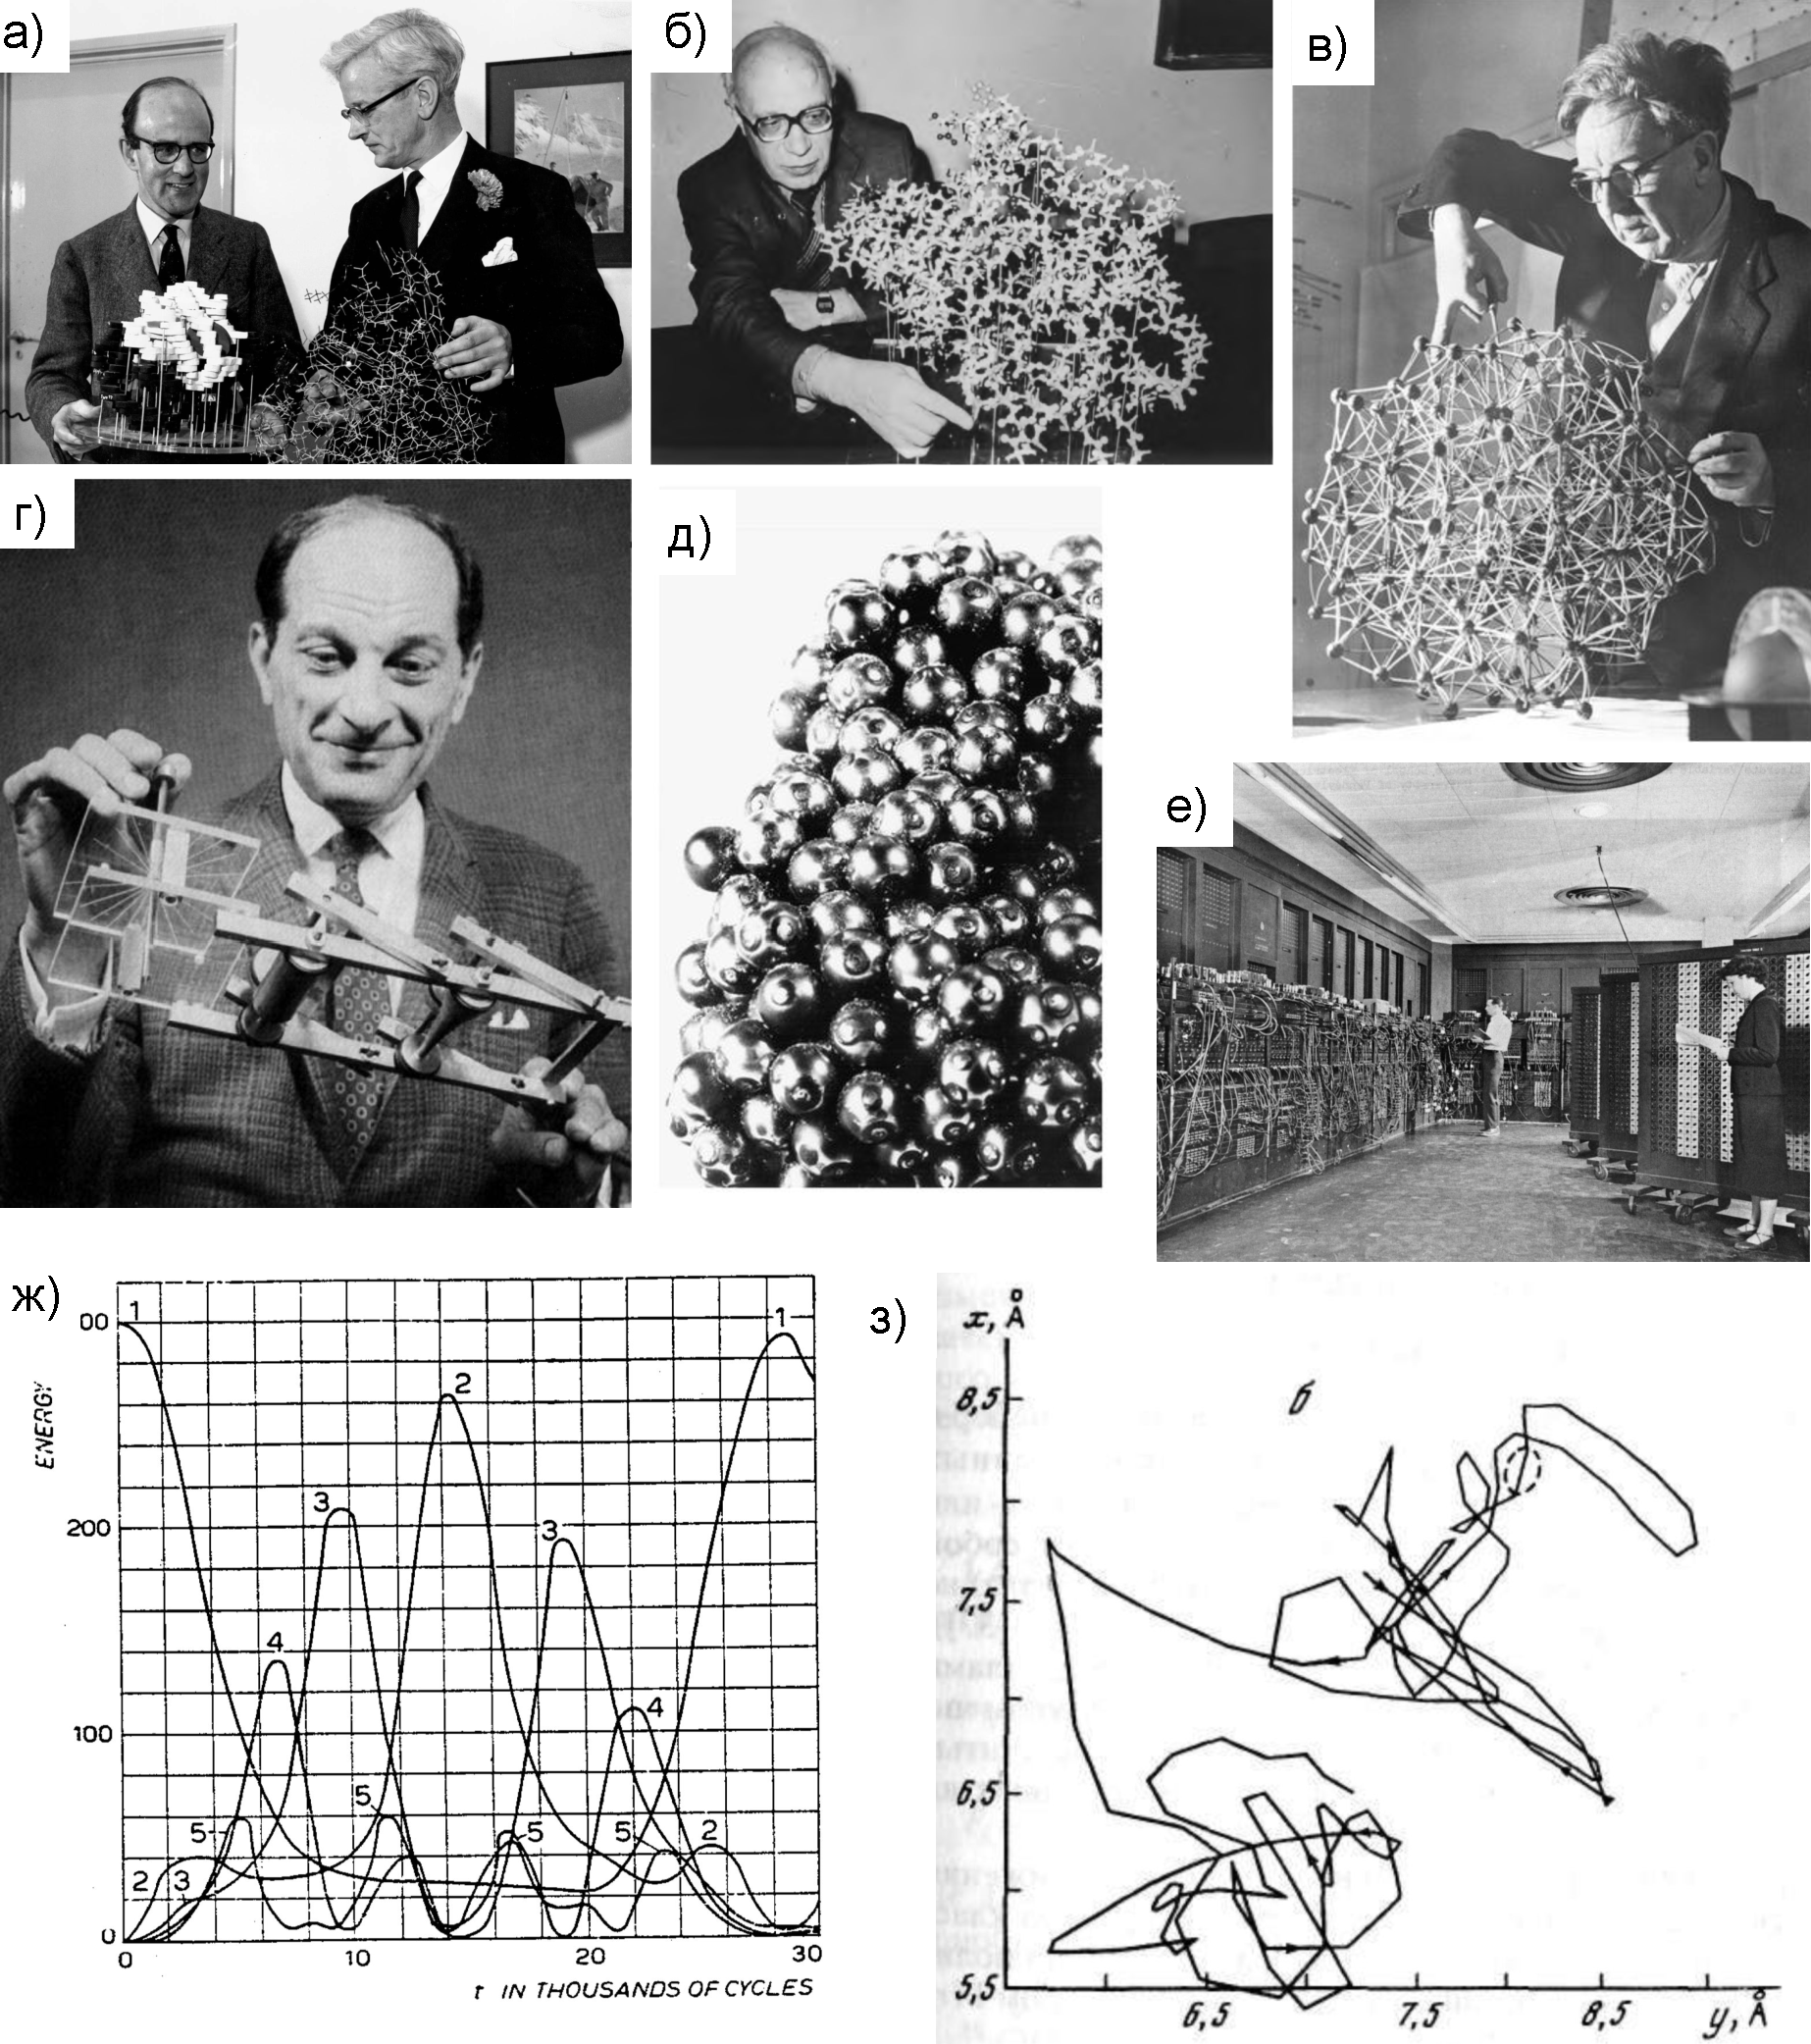
\includegraphics [width=350pt] {images/p1/mod_history.pdf}
  \caption[Иллюстрации к истории структурной биологии и моделирования.]{Иллюстрации к истории структурной биологии и моделирования. а) М. Перуц (слева) и Д. Кендрю (справа) со структурными моделями миоглобина. б) Б.К. Вайнштейн со структурой белка \cite{kovalchuk__2012}, в) Дж. Д. Бернал с моделью укладки атомов в жидкости \cite{finney_bernals_2013}, г) С. Улам с тележкой Монте-Карло Энрико Ферми \cite{gregg_mncp_nodate},  д) результаты физического моделирования жидкости в виде стальных шаров в работах Д.Д. Бернала \cite{finney_bernals_2013}, е) первый программируемый компьютер общего назначения ENIAC \cite{noauthor_english_1947}, ж) изменение полной энергии со временем для первых пяти мод вибрирующей струны в задаче Ферми-Пасты-Улама-Цингу, первая работа по исследованию статистических свойств механических систем методом молекулярной динамики, 1955 г. \cite{fermi_studies_1955}, (з) Траектории движения атомов в жидкости, рассчитанные методом МД из кандидатской диссертации А.Г. Гривцова, начало 1970-ых годов \cite{grivtsov_metodika_1996}.} 
  \label{fig:p1:mod_history}
\end{figure}

%%% ссылка на гривцова - обзорная статья маленкова https://www.google.com/url?sa=t&rct=j&q=&esrc=s&source=web&cd=&ved=2ahUKEwjrk6OPxcXrAhVI_SoKHTF5ACcQFjAAegQIBRAB&url=https%3A%2F%2Fistina.msu.ru%2Fdownload%2F101116065%2F1gBMHJ%3AYj-jpNMcPPBJ8nZ6Q-g4XcwGQIU%2F&usg=AOvVaw0_u1y_ZMajjPhNvAxlFsSa

%историческая статью о Монте Карло из LANL https://permalink.lanl.gov/object/tr?what=info:lanl-repo/lareport/LA-UR-88-9068
% а это статья метрополиса https://permalink.lanl.gov/object/tr?what=info:lanl-repo/lareport/LA-UR-88-9067
%также в вики неплохой обзор в биографии улама
%https://en.wikipedia.org/wiki/Stanislaw_Ulam#Manhattan_Project

%FERMIAC

%МД история
% https://en.wikipedia.org/wiki/Molecular_dynamics#History
% ферми улам (там картинка есть), затем Алдер, Раман (посмоьореть статьи)

% что-то из статьи гривцова - балабаева


Сам по себе термин \textit{молекулярное моделирование} (\textit{molecular modeling}) является достаточно широким понятием, значение которого постепенно расширяется и видоизменяется с развитием различных новых методов. В одних случаях упор может делаться непосредственно на задачу создания модели (например, пространственной модели белка), в других случаях на анализ и исследование свойств молекул на основе физических моделей поведения и взаимодействия атомов. К первому типу задач можно отнести традиционные задачи реконструкция структуры биомакромолекул по экспериментальным данным. Данный процесс всегда включает в себя шаг создания модели, которая удовлетворяет этим данным. На заре структурной биологии реконструкция биомолекул по результатам кристаллографических экспериментов долгое время сводилась к построению пространственных моделей из проволоки, дерева, других материалов (Рис. \ref{fig:p1:mod_history}aб). Позднее данный процесс был значительно автоматизирован с применением компьютерных технологий, разработаны соответствующие программные пакеты по автоматизации построения моделей и их визуализации (например, CCP4 \cite{winn_overview_2011}, O, Phenix \cite{liebschner_macromolecular_2019}, Coot  \cite{emsley_coot_2004}, Pymol \cite{schrodinger_pymol_2015}, Chimera \cite{pettersen_ucsf_2004}).  Построение моделей молекул в виде пространственного расположения атомов, удовлетворяющего набору экспериментальную данных, - одно из возможных значений термина компьютерное молекулярное моделирование. 
В то же время со времен возникновения молекулярно-кинетической теории (основы которой были в том числе заложены М.В. Ломоносовым \cite{lomonosov_sobranie_1950})
ученые стремились к описанию и предсказанию свойств молекулярных систем на основе учета взаимодействий между отдельными атомами, описываемых законами физики. В до-компьютерную эпоху такие предсказания можно было делать либо на основе теоретических расчетов, либо на основе физических механических моделей. Так, например, в 1950-60-ых годах для молекулярного моделирования жидкостей Джон Десмонд Бернал активно использовал механические модели в виде металлических и пластиковых шариков \cite{bernal_bakerian_1964}(Рис. \ref{fig:p1:mod_history}вд)\footnote{Любопытным также является факт, что тот же Дж. Д. Бернал является одним из основателей области биомолекулярной кристаллографии, под его руководством работали классики структурной биологии Макс Перутц, Дороти Ходжкин, Розалинд Франклин \cite{breathnach_desmond_1995}, а также в честь него назван пакет по молекулярному моделированию DESMOND \cite{kevin_schrodinger_2020}.}. С развитием компьютерных технологий появились возможности численного моделирования поведения молекулярных систем на основе их физических моделей. Следует отметить, что в английском языке для описания такого рода деятельности активно используется термин \textit{molecular simulations} (см. например \cite{Frenkel}), который на русский язык обычно переводится также ``молекулярное моделирование'', однако слово ``simulations'' имеет важные отличия в своей смысловой нагрузке. Под этим термином понимается не столько создание моделей, сколько изучение и анализ теоретических моделей с помощью вычислительных методов, так называемые ``вычислительные эксперименты''. В области инженерного моделирования в русском языке для обозначения термина ``simulation modeling'' используется термин \textit{имитационное моделирование}, однако он не вошел в обиход в среде исследователей, занимающихся молекулярным моделированием. Подход к изучению различных систем на основе проведения вычислительных экспериментов на данный момент многими воспринимается как одна из парадигм научного познания наравне с экспериментальным и теоретическими подходами \cite{hey_fourth_2009} и получил название \textit{in silico} подхода. В случае изучения свойств вещества данный подход предполагает наличие определенной физической модели исследуемого объекта, которая описывает взаимодействия между его составными частями, и использует различные вычислительные алгоритмы, чтобы исследовать свойства данной модели вещества. Если для описание физической модели вещества используются различные приближения, основанные на законах квантовой механики, то такие подходы зачатую называют \textit{ab initio} подходами (от лат. ``из первых принципов'' - подразумевая, что для моделирования необходимо знать лишь базовые физические константы). Для моделирования многих задач и веществ такой формализм является слишком вычислительно затратным, поэтому исторически область ``molecular simulations'' развивалась в первую очередь на основе формализма классической механики (частицы вещества представлялись в виде материальных точек, взаимодействующих по законам классической механики).

Зарождение области вычислительных экспериментов в молекулярном моделировании происходило в середине-конце 1940-ых годов во время работы над созданием ядерного и термоядерного оружия в США  и связано в первую очередь с именами Станислава Улама, Джона фон Неймана, Николаса Метрополиса, а также с вводом в строй в 1945 году первого электронного цифрового вычислителя общего назначения ENIAC (Рис. \ref{fig:p1:mod_history}е). С. Улам и Д. фон Нейман, работая над проблемой транспорта нейтронов в различных типах ядерных систем, предложили в 1947 году моделировать диффузию нейтронов путем многократного численного расчета траекторий движения отдельных нейтронов с учетом случайности их взаимодействия с окружающим веществом. Таким образом, решение задачи о вычислении средних характеристик данного процесса сводилось к статистической выборке (statistical sampling), а не к полному численному решению уравнений, которые описывали этот процесс. Благодаря наличию компьютера ENIAC  стало возможным написать компьютерную программу для соответствующих расчетов, которая использовала в том числе генератор псевдослучайных чисел для моделирования случайных событий и соответствующих статистических выборок \cite{eckhardt_and_1987}.  Подходы основанные на статистическом моделирования с использованием случайных величин были названы ими методомами Монте-Карло, по предложению Николаса Метрополиса, а первая статья по этому методу опубликована в 1949 году \cite{metropolis_monte_1949}. Любопытным является факт, что физик Энрико Ферми еще до формулировки метода Монте Карло Уламом и фон Нейманом использовал метод статистических выборок для своих задач, проводя расчеты вручную в предрассветные часы, когда страдал бессонницей \cite{metropolis_beginnig_1987}. В 1947 году, когда постановка расчетов на компьютере ENIAC была временно невозможной из-за его перевозки, Ферми придумал аналоговый компьютер, который можно было использовать для моделирования транспорта нейтронов. Данный компьютер представлял собой тележку с карандашом, которую нужно было передвигать по бумажному чертежу и периодически изменять ее направление на основе случайных чисел, таким образом моделируя передвижения нейтронов и их столкновения с атомами среды. Данное устройство получило название тележки Монте-Карло или FERMIAC (см Рис. \ref{fig:p1:mod_history}г).

Следующей важной вехой в развитии методов Монте Карло в молекулярном моделировании и статистической механике явилась разработка Метрополисом, супругами Розенблют и Теллер в 1953 году метода Монте Карло на основе марковских цепей (Markov Chain Monte Carlo, MCMC) для изучения уравнений состояния вещества состоящего из индивидуальных взаимодействующих молекул \cite{metropolis_equation_1953}. В этой работе авторы провели исследование двумерного газа из жестких сфер на компьютере MANIAC. Инновацией данного метода стало вычисление статистической выборки состояний согласно распределению Больцмана в многомерном пространстве через построение марковской цепи состояний. Случайные переходы между состояниями принимались или отклонялись согласно критерию Метрополиса-Хастингса таким образом, что лимитирующее распределение состояний в данной марковской цепи соответствовало Больцмановскому распределению состояний по энергиям. На идеях данной работы основано большинство подходов по моделированию молекулярных систем методами Монте Карло и в наши дни \cite{ivanov_methods_2009}.

1950-ые годы также ознаменовалось первыми работам в области применения метода молекулярной динамики - численного решения уравнений движения классической механики. 
Впервые Ферми, Паста, Улам и Цингу исследовали колебания струны с нелинейной упругостью и показали наличие необычной периодичности возникающей в нелинейных системах \cite{fermi_studies_1955}. 
Идея моделирования динамики молекулярных систем была сформулирована Олдером и Вайнрайтом в 1957 году -- с помощью компьютера UNIVAC исследовались фазовые переходы в системе твердых сфер \cite{alder_phase_1957}. К первым попыткам применить методы молекулярной динамики к реалистичным системам можно отнести работу Гибсона и др. 1960 года по моделированию радиационного поражения меди \cite{gibson_dynamics_1960} и работу Aнисура Рамана по моделированию жидкого аргона 1964 года \cite{rahman_correlations_1964}. В нашей стране первые шаги по развитию методов молекулярной динамики связаны с деятельностью А.А. Гривцова, Э.Э. Шноля, Н.К. Балабаева из Института прикладной математики (ИПМ, Москва) начиная с 1967 года \cite{grivtsov_metodika_1996}. С тех пор методы молекулярной динамики стали активно применяться для моделирования газов, жидкостей \cite{allen_computer_1989}, а  позднее стали активно применяться и для моделирования биомакромолекулярных систем. Развитие применения методов молекулярного моделирования к биомолекулярным системам связаны с деятельностью групп Мартина Карплуса, Арье Варшеля, Майкла Левитта, которые получили в 2013 году нобелевскую премию за ``разработку мультимасштабных моделей сложных химических систем'', а также групп Питера Коллмана, Хермана Берендсена, Клауса Шультена, Дэвида Кейса, Эрика Линдаля, Алекса МакКерела и др. Работы группа М. Карплуса легли в основу набора силовых полей CHARMM, a также одноименной программы для моделирования \cite{karplus_molecular_2003}. На основе подходов, силовых полей и программного кода CHARMM были развиты многие родственные программы, например, программа для параллельных расчетов молекулярной динамики NAMD (в группе К. Шультена) \cite{phillips_scalable_2020}, программа для моделирования на основе данных ЯМР XPLOR \cite{schwieters_xplor-nih_2003}, программа для моделирования по гомологии MODELLER \cite{sali_comparative_1993}. Работы группы Питера Коллмана положили основу программному пакету AMBER и одноименной группе силовых полей \cite{case_amber_nodate}. Работы группы Хермана Берендсена в Голландии заложили основы пакета по моделированию GROMACS \cite{lindahl_gromacs_2020} и силового поля GROMOS \cite{soares_improved_2005}. В нашей стране развитие программных продуктов в области молекулярной динамики связано в том числе с разработкой программы PUMA и ее версий под руководством Н.К. Балабаева \cite{likhachev_parallelism_2018}.

В первые десятилетия XXI века область молекулярного моделирования продолжала активно развиваться и совершенствоваться, в том числе и в методологическом плане. Стоит отметить адаптацию программного обеспечения для использования массивно-параллельных архитектур графических процессоров, что позволило уверенно проводить расчеты МД в микросекундном диапазоне не только на суперкомпьютерах, но и отдельных рабочих станциях \cite{noauthor_nvidia_nodate}.  Усилиями нескольких групп создавались специализированные компьютерные платформы для расчета молекулярной динамики, в частности архитектуры MD GRAPE в Японии \cite{ohmura_mdgrape-4_2014} и компьютеры ANTON компании D.E. Shaw Research \cite{shaw_anton_2014}. Последние позволяют проводить вычисления в миллисекундном диапазоне времен моделируемых систем.

Серьезный прогресс был достигнут и в совершенствовании методов повышения эффективности статистических выборок (enhanced sampling methods) в ходе расчетов молекулярной динамики. К таким методам можно отнести методы метадинамики (metadynamics) \cite{laio_escaping_2002}, адаптивной смещающей силы (adaptive biasing force) \cite{lesage_smoothed_2017}, адаптивно смещаемой молекулярной динамики (adaptevly biased molecular dynamics) \cite{marchi_adiabatic_1999}, динамики с обменом репликами (replica exchage molecular dynamic/parallel tempering) \cite{sugita_replica-exchange_1999}, управляемой молекулярной динамики (steered molecular dynamics) \cite{shaytan_neravnovesnaya_2006}. Многие из этих методов получили активное распространение благодаря созданию кросс-платформенного дополнения к пакетам молекулярной динамики PLUMED \cite{bonomi_promoting_2019}. Были в том числе развиты теоретические основы, связывающие характеристики расчета неравновесных молекулярных процессов с равновесными параметрами моделируемых системы. К таковым можно отнести равенство Джарзинского, связывающее работу в ходе неравновесного процесса над системой с разницей свободной энергии между конечным и начальным состояниями \cite{jarzynski_nonequilibrium_1997} и флуктуационную теорему Крукса (Crooks fluctuation theorem)\cite{crooks_entropy_1999}. Любопытно, что открытие и формулировка данных достаточно лаконичных и простых соотношений неравновесной статистической физики произошла только на рубеже XX и XXI веков, хотя явные предпосылки для их формулировки существовали со времен Больцмана. Отдельно стоит отметить развитие и успехи различных эмпирических подходов к моделированию структуры и дизайну белков. В отличие от методов, исходящих в первую очередь из физических представлений о структуре, подвижности и взаимодействии атомов в боимакромолекулах  (physics-based methods), такие подходы активно используют различные эмпирические скоринговые функции для оценки вероятности той или иной конформации белка, которые основываются на статистическом анализе большого количества уже известных пространственных структур белков, а также эволюционном анализе похожести различных аминокислотных мотивов в белках. Перебор конформационного пространства полипептидной цепи также зачастую ограничивают набором конформаций фрагментов присутствующих в уже известных структурах белков. К таким методам можно отнести подходы основанные на пакете ROSETTA \cite{leman_macromolecular_2020}, AWSEM-MD \cite{wu_awsem-idp_2018} и др.

Выше мы обсудили в историческом контексте различные взгляды на задачи и методы молекулярного моделирования. В одном случае речь идет о задачах поиска оптимальной пространственной модели молекулы на основе большого количества экспериментальных данных (например, реконструкции структуры белка по набору рефлексов картины дифракции его кристаллов), в другом случае упор делается на имитационное моделирования (molecular simulations) систем на основе физических моделей взаимодействий между атомами, которые иногда называют также \textit{ab inito} подходами (напр. \textit{ab initio protein folding}\footnote{Не стоит путать с пониманием термина \textit{ab initio} в квантовой химии, где под этим понимается моделирование на основе решения уравнения Шредингера.} и т.д.).
Разные аспекты данных подходов просуммированы на рисунке \ref{fig:p1:concept_matrix}, они отличаются по наличию, качеству и информационному содержанию используемых экспериментальных данных (Рис. \ref{fig:p1:concept_matrix}в), по используемым математическим подходам и физическим теориям (Рис. \ref{fig:p1:concept_matrix}б) и по самому представлению моделей (Рис. \ref{fig:p1:concept_matrix}а) - в одном случае речь обычно идет о некоторой статической структуре или наборе структур, в другом о статистических ансамблях различных конформаций.
% мнение Кейса про розетту https://onlinelibrary.wiley.com/doi/full/10.1002/cmr.a.21403


В то же время в структурной биологии существует большое количество задач, которые не решаются в рамках одного из двух вышеописанных подходов. С одной стороны для многих систем, экспериментальные данные могут присутствовать лишь в ограниченном количестве и зачастую иметь опосредованное отношение к деталям молекулярной структуры (напр. данные спектроскопических экспериментов, где оценивается взаимодействие введенных в структуру меток, данные по химической доступности и реакционной способности различных групп, данные малоуглового рассеяния и т.д.). С другой стороны, решение структурных задач напрямую \textit{in silico} методами физического моделирования на основе взаимодействия частиц невозможно для большинства систем в силу чрезвычайной вычислительной сложности и зачастую качества имеющихся моделей взаимодействия атомов в биомакромолекулах. Отдельную проблему представляют задачи описания структуры биомакромолекул, у которых нет явной статической структуры, а она представлена ансамблем конформаций. К примерам таких систем можно отнести внутренне разупорядоченные белки (англ. intrinsically disordered proteins), а также большинство биомакромолекулярных комплексов (вплоть до структуры хроматина на масштабах клеточного ядра) -- по мере роста размеров комплексов, они все реже формируют какую-то одну статическую конформацию, а их функционирование завязано сложную внутри- и межмолекулярную динамику. Для описания таких молекул динамический формализм используемый в имитационном молекулярном моделировании (molecular simulations) подходит значительно лучше, однако зачастую решение таких задач из первых принципов опять сводится к вышеописанным затруднением.

\begin{figure}[H] 
  \center
  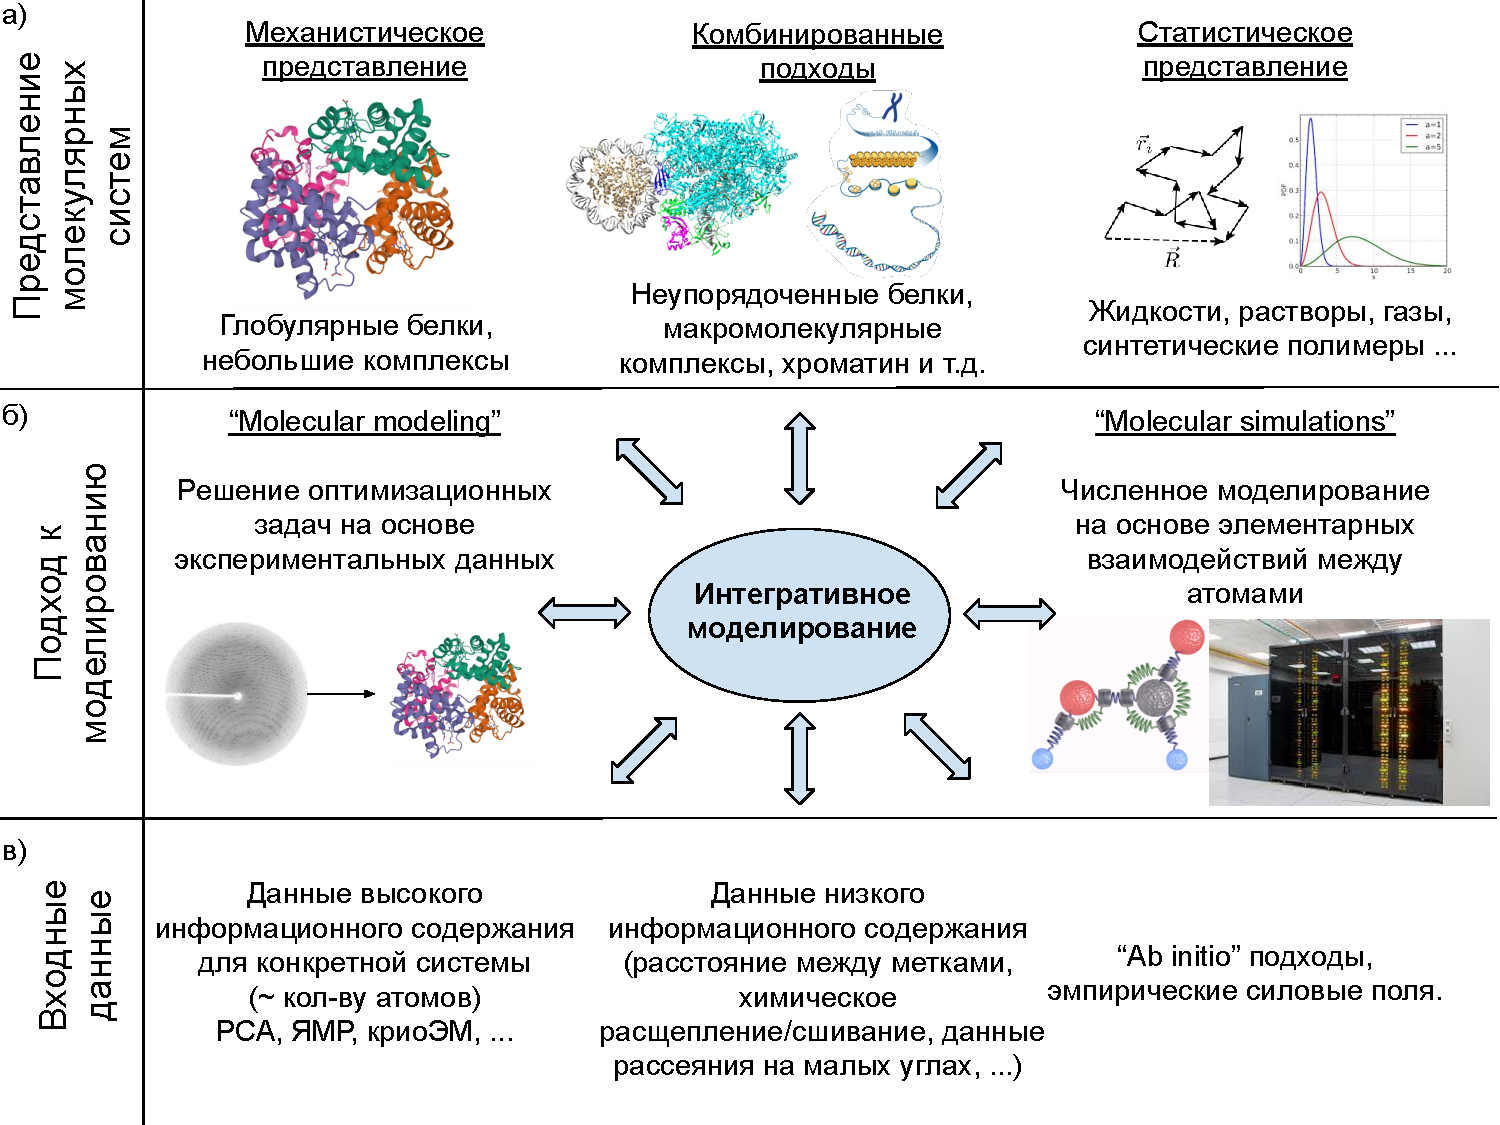
\includegraphics [width=\textwidth] {images/p1/concept_matrix.pdf}
  \caption{Диаграмма, суммирующая различные подходы к описанию, моделированию и изучению структуры и динамики биомакромолекул.} 
  \label{fig:p1:concept_matrix}
\end{figure}



Таким образом, актуальным является разработка гибридных методов и подходов по моделированию биомакромолекулярных комплексов, которые сочетают возможности построения структурных моделей как на основе экспериментальных данных (в том числе данных с низким информационным содержанием), так и на основе моделирования атом-атомных взаимодействий, а также учитывают структурные динамические особенности многих биомакромолекулярных систем. Такие подходы в последнее время в литературе получили название \textit{интегративного моделирования} (от англ. integrative modeling, см. напр. \cite{braitbard_integrative_2019}). Одной из задач интегративного моделирования является в том числе интеграция различного рода экспериментальных данных при построении моделей биомакромолекулярных систем. На Рис. 
\ref{fig:p1:int_mod} представлены различные типы экспериментальных данных, которые могут быть использованы в интегративном моделировании. К ним  могут относится структуры биомакромолекул или отдельных их частей полученные традиционными методами структурной биологии с высоким разрешением, а также набор данных низкого информационного содержания (когда данных недостаточно для реконструкции структуры традиционными методами), полученных различными биофизическими, биохимическими и другими методами. К последним могут относится данные полученные методами электронной микроскопии низкого разрешения, данные малоуглового рассеяния рентгеновских лучей или нейтронов, данные о взаимодействии введенных в структуру меток, получаемые методами ЯМР, ЭПР, спектроскопии Ферстеровского резонансного переноса энергии (FRET spectroscopy), данные по экспонированности в растворитель различных групп биомакромолекул, получаемые на основе экспериментов по дейтеро-водородному обмену, данные экспериментов по химическому сшиванию или разрушения биомакромолекул, данные получаемые с применением методов геномики (например, методов ChIP-seq, Hi-C и др.). Актуальной является и задача обратного рода -- имея некоторую структурно-динамическую модель биомакромолекулярной системы, рассчитать параметры ее отклика в различных типах экспериментов (см. Рис. \ref{fig:p1:int_mod}). Обсуждаемые подходы также важны при дизайне и конструировании новых биомакромолекулярных комплексов с полезными функциями.

Данная диссертационная работа посвящена развитию вышеописанных подходов интегративного моделирования. В работе представлены различные элементы интегративного подхода. В главе \ref{part2_supermd} рассмотрены работы по использованию суперкомпьютерных расчетов методом атомистической молекулярной динамики для изучения динамики биомакромолекулярных комплексов на основе уже известных пространственных структур, в главе \ref{part5_hrf} рассмотрены работы по интегративному моделированию нуклеосом на основе данных расщепления ДНК гидроксильными радикалами (hydroxyl-radical footprinting), в главе \ref{part6_nucl_complex} рассмотрены работы по созданию моделей комплексов нуклеосом с белками хроматина на основе разнообразных экспериментальных данных, в главе \ref{part4_amyloid} рассмотрены работы по интегративному моделирования амилоидоподобных фибрилл.

Последующие разделы данной главы будут посвящены изложению ряда методических основ методов молекулярного моделирования, которые использовались автором в ходе решения научных задач, излагаемых в данной диссертации, а также изложению основ некоторых экспериментальных методов, данные которых использовались автором в работах по интегративному моделированию биомакромолекулярных комплексов.



\begin{figure}[H] 
 \center
 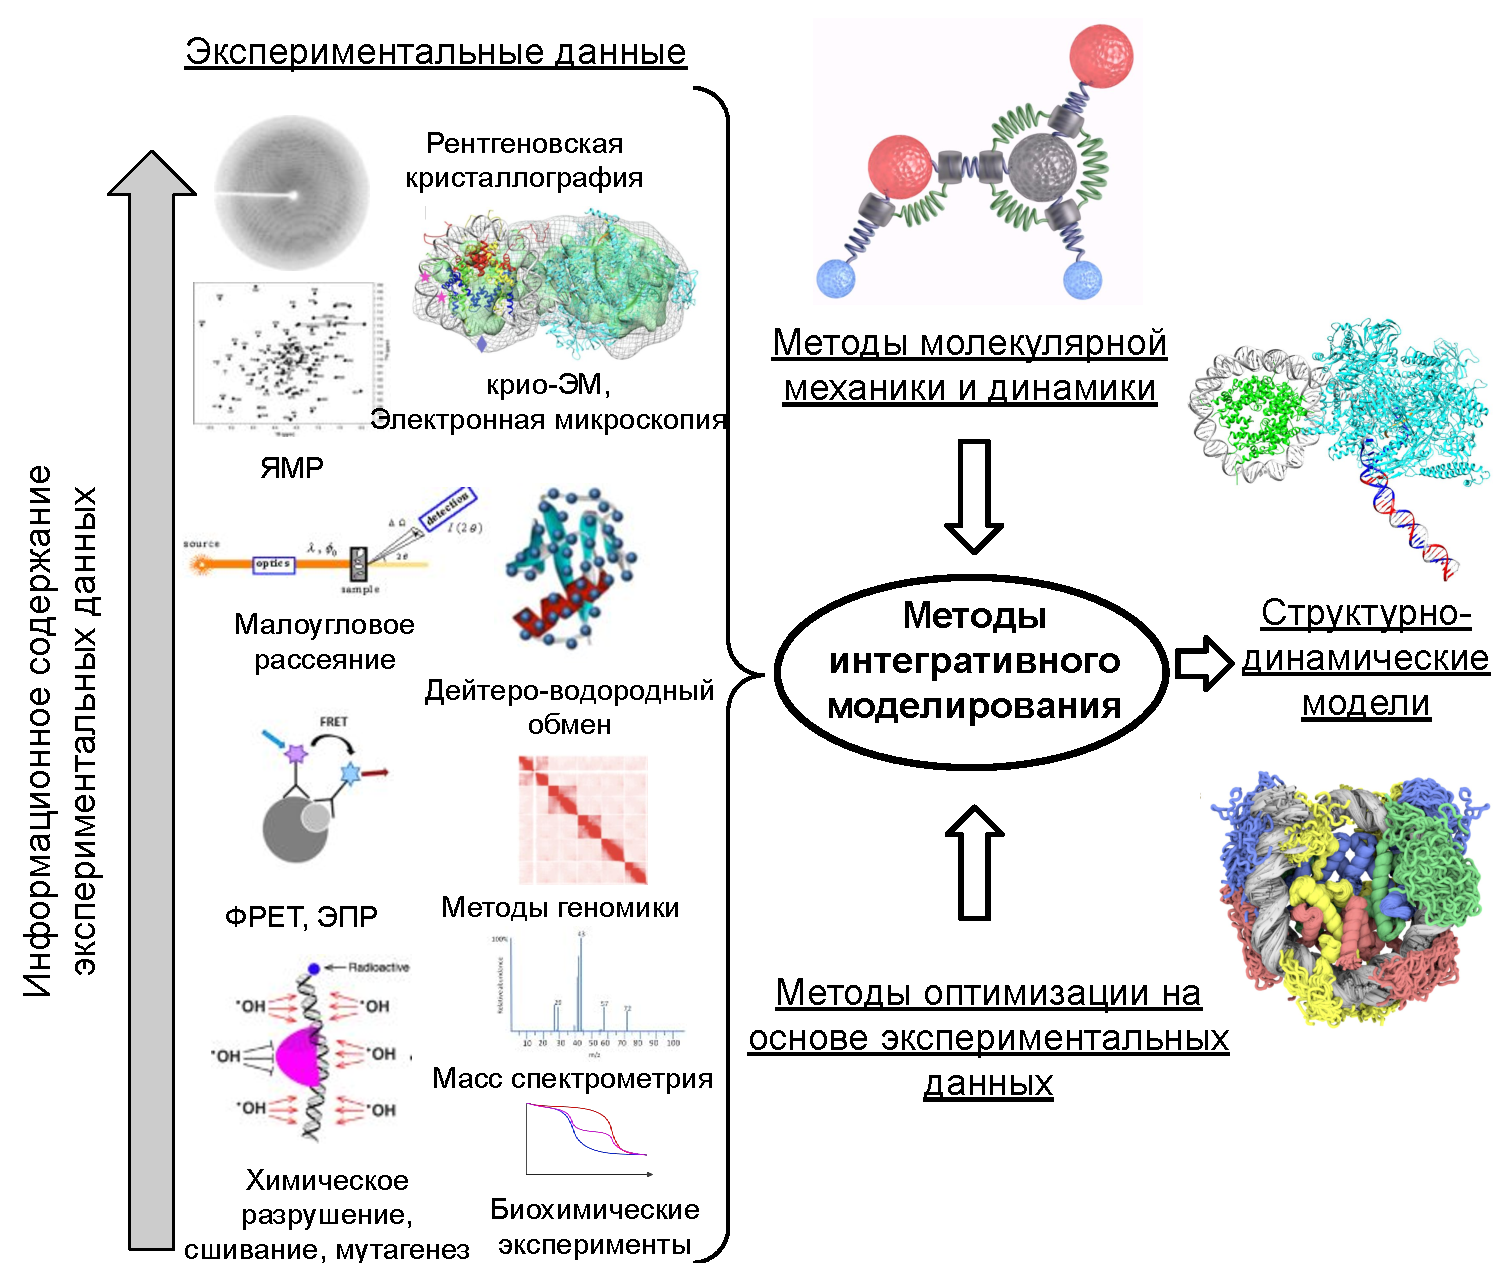
\includegraphics[width=\textwidth] {images/p1/int_mod.pdf}
 \caption{Идея методов интегративного моделирования.} 
 \label{fig:p1:int_mod}
\end{figure}



%Дальнейшая логика главы



% Методы молекулярной динамики и механики - взять из кфмн + добавить из немецкой
%расчет своб энергии - из кфмн
%мол поверхности из кфмн
% из диссертации армеева нужно взять про ДНК
% и про монте карло
%? что-то про метаД????
% Основы экспериментальных методов
%% ФРЕТ
%% Гидрокс
%% Электронка???
%%ЯМР???
%% Малоугл? (было ли в JMB)

%\section{Методы суперкомпьютерного атомистического моделирования } %%или \section{Методы молекулярной механики и динамики}
\section{Методы атомистического суперкомпьютерного моделирования} \label{part1_1_md}
\textit{Начало раздела \ref{part1_1_md} и раздел \ref{part1_1_md}.1 изложены согласно кандидатской диссертации автора \cite{shaytan_thesis_kfmn_2010} << }

О методах классического молекулярного моделирования написано множество подробных книг и монографий (см. например \cite{Frenkel,allen_computer_1989}), поэтому ниже мы лишь кратко обсудим основные понятия и подходы.

В основе методов классических атомистических методов молекулярного моделирования лежит представление о молекулярной структуре как о наборе классических частиц (материальных точек или в некоторых случаях твёрдых тел) взаимодействующих по законам классической механики. Молекулярно-механическая модель обычно предполагает следующие приближения: (i) электронные степени свободы не учитываются, а учитываются лишь атомные степени свободы, (ii) молекулы полагаются находящимися в основном энергетическом состоянии, (iii) автоматически предполагается приближение Борна-Оппенгеймера. На практике при задании конкретных типов взаимодействий между атомами в виде молекулярного гамильтониана предпринимается ещё ряд серьёзных приближений.

В случае моделирования биомолекулярных систем в приближении классической механики методические основы можно грубо разделить на три больших области: 1) задание механистической модели молекулярной системы на основе набора параметров, называемого силовым полем, 2) задание метода изучения динамики системы или метода изучения конформационного пространства данной системы, 3) различные технические и алгоритмические детали, связанные с эффективным и быстрым расчетом взаимодействий между атомами, а также оптимизацией расчетов на различных вычислительных системах.


%Ниже текст из файла materials/thesis_portable.pdf, ссылки надо смотреть там, но я их всех уже импортировал в зотеро.
%\todo{2S - из файла materials/thesis\_portable.pdf взять текст и картинки начиная со стр. 31 со слов "In molecular mechanics molecular system" до конца 39 страницы. с картинками и формулами. ссылки надо смотреть там, но я их всех уже импортировал в зотеро.}

\subsection{Силовые поля}
В молекулярной механике молекулярная система описывается в терминах классической механики набором точечных частиц (обычно представляющих атомы или группы атомов) и их взаимодействий, заданных функцией потенциальной энергии. Форма и структура функции потенциальной энергии называется силовым полем. На сегодняшний день разработано большое количество различных типов силовых полей, от обычных силовых полей до силовых полей, специфичных для определенного класса соединений. К наиболее популярным относятся группы силовых полей OPLS-AA \cite{jorgensen_development_1998}, AMBER \cite{cornell_2nd_1995}, CHARMM \cite{mackerell_all-atom_1998}, GROMOS \cite{schuler_improved_2001} , CVFF \cite{dauber-osguthorpe_structure_1988}, PCFF \cite{sun_force_1994}, MM3 \cite{allinger_molecular_1989} и другие. Эти силовые поля могут быть параметризованы относительно экспериментальных данных (в частности, калориметрических, спектроскопических), а также для воспроизведения поверхностей потенциальной энергии, вычисленных с помощью методов квантовой химии. Сложность функциональной формы силового поля может варьироваться, однако почти все молекулярные силовые поля содержат шесть общих основных термов для описания валентных и невалентных взаимодействий. Среди валентных взаимодействий выделяют термы описывающие растяжения ковалентных связей, деформации валентных углов, торсионных углов и ложноторсионные углы. Невалентные взаимодействия обычно описываются комбинацией парных ван-дер-Ваальсовых взаимодействий и кулоновских взаимодействий, основанных на точечных частичных зарядах атомов. Рисунок \ref{fig:p1_1:f10} и уравнение \ref{eq:p1_1:e1} дополнительно иллюстрируют эти термы. Многие из обычных силовых полей, используемых для моделирования биомолекул, включают в себя только упомянутые выше основные энергетические термины. Более сложные силовые поля (например, MM3, PCFF) могут также включать ангармонические члены и перекрестные члены для валентных взаимодействий, которые отражают связь между внутренними координатами. Например, при уменьшении валентного угла между атомами обнаруживается, что валентные связи удлиняются, чтобы уменьшить взаимодействие между атомами. Было обнаружено, что перекрестные члены играют важную роль в силовых полях, предназначенных для предсказания колебательных спектров  \cite{leach_molecular_2001}. Было высказано предположение, что наличие перекрестных членов (вместе с некоторыми другими особенностями) может обеспечить общий способ классификации силовых полей \cite{hwang_derivation_1994}. Согласно этой логике, силовое поле класса I ограничено гармоническими членами (например, для растяжения связей и валентного угла) и не имеет перекрестных членов. Силовое поле класса II будет иметь ангармонические члены и явные перекрестные члены для учета взаимоотношений между различными геометрическими параметрами. Еще одной характеристикой силового поля класса II считается возможность его использования без модификации одновременно для моделирования свойств изолированных малых молекул, конденсированных фаз и макромолекулярных систем \cite{leach_molecular_2001}.
\begin{multline}
    U(\{\vec{r}_i\})= \sum_{bonds} \frac{1}{2} k_b (l-l_0)^2  + \sum_{angels} \frac{1}{2}k_\theta (\theta - \theta_0)^2 + \sum_{torsions} \frac{1}{2} V_n [1+\cos({n\varphi-\varphi_0})] + \\
     \sum_{impropers} \frac{1}{2} k_\gamma (\gamma-\gamma_0)^2 + \sum_{j+1}^{N-1} \sum_{i=j+1}^{N} \Bigg\{ 4\epsilon_{ij} \Bigg[\Big(\frac{\sigma_{ij}}{r_{ij}}\Big)^{12} - \Big(\frac{\sigma_{ij}}{r_{ij}}\Big)^6\Bigg] + \frac{q_iq_j}{4\pi \epsilon_0 r_{ij}} \Bigg\} f_{ij}
     \label{eq:p1_1:e1}
\end{multline}

\begin{figure} [h!]
    \centering
    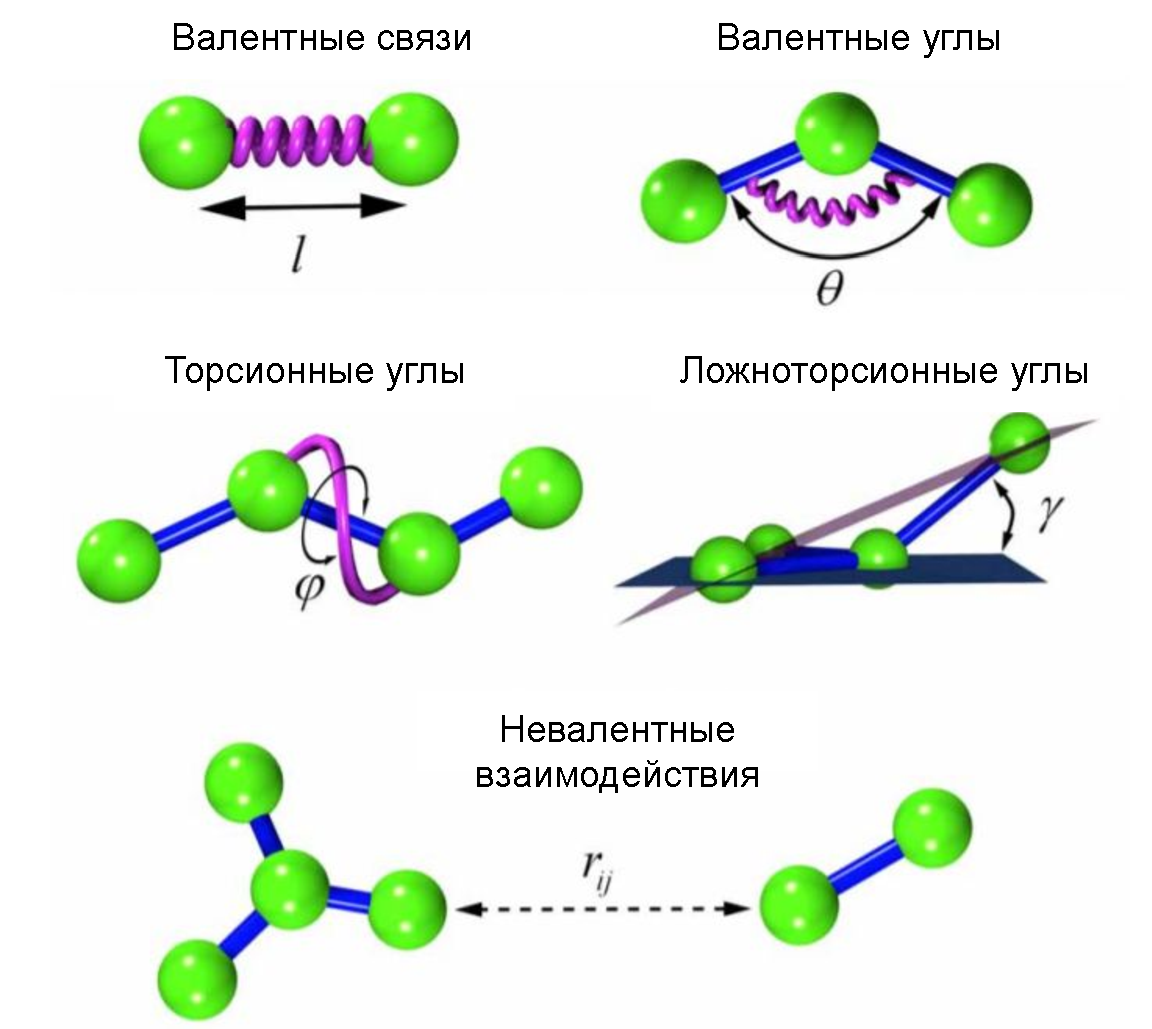
\includegraphics [width=\textwidth]{images/p1/part1_1_md/part1_1_md_f10.pdf}
    \caption[Энергетические термы силового поля]{Графическое изображение энергетических термов в силовых полях молекулярной механики. Атомы изображены зелеными сферами. Рисунок соответствует членам, представленным в уравнении 
    \ref{eq:p1_1:e1}}
    \label{fig:p1_1:f10}
\end{figure}


\subsubsection{Силовое поле OPLS-AA}
В качестве примера устройства типичного силового поля, применяемого для моделирования белков и других биологических молекул, рассмотрим поле OPLS-AA. Силовое поле OPLS-AA \cite{oplsaa,oplsaa2} является полноатомной версией поля OPLS (Optimized Potentials for Liquid Simulations), то есть атомы водорода рассматриваются явным образом. Параметры поля OPLS, в частности, подгонялись под экспериментальные свойства жидкостей, таких как плотность и теплота испарения.
Общая структура энергии молекулярной системы представлена в уравнении \ref{opls_ff_eqn}.

\begin{eqnarray}
&&U(r^N)=U_{bond}+U_{angle}+U_{dih}+U_{nb} \label{opls_ff_eqn}\\
&&U_{bond}=\sum_{bonds}K_r (r-r_{eq})^2\nonumber\\
&&U_{angle} = \sum_{angles} k_\theta \left ( \theta - \theta_{eq} \right )^2\nonumber\\
&&U_{dih} = \frac {V_1} {2} \left [ 1 + \cos \left ( \phi \right ) \right ] 
                + \frac {V_2} {2} \left [ 1 - \cos \left ( 2 \phi \right ) \right ] 
                + \frac {V_3} {2} \left [ 1 + \cos \left ( 3 \phi \right ) \right ] 
                + \frac {V_4} {2} \left [ 1 - \cos \left ( 4 \phi \right ) \right ]\nonumber\\
&&U_{nb}^{ab} = \sum_{i} ^{on\ a} \sum_{j} ^{on\ b} \left \{
                    4 \epsilon_{ij} \left [ \left( \frac {\sigma_{ij}}{r_{ij}} \right )^{12} 
                    - \left ( \frac {\sigma_{ij}}{r_{ij}} \right )^6 \right ]  + \frac {q_iq_j} {r_{ij}}
                   \right \} f_{ij}\nonumber
\end{eqnarray}
межмолекулярные взаимодействия $U_{nb}$ учитываются только для атомов, которые удалены на три и более связи, для 1-4 взаимодействий коэффициент скейлинга $f_{ij}=0.5$, во всех остальных случаях $f_{ij}=1$.

\subsubsection{Силовое поле PCFF}
Силовое поле PCFF (Polymer Consistent Force Field) \cite{pcff_sun_1994} основано на силовом поле CFF91 и относится к семейству силовых полей CFF (consistent force-field). Это поле создано для моделирования широкого класса органических полимеров, утверждается, что силовые поля второго поколения (к которым относится PCFF) более точно воспроизводят экспериментальные результаты, чем силовые поля первого поколения. Платой за это является более сложное устройство поля и наличие перекрёстных членов в функции энергии. Общий вид энергии молекулярной системы в приближении поля PCFF приведён в формулах \ref{pcff_eqn}. На Рис. \ref{fig:2_pcff_terms} приведено графическое пояснение к внутренним степеням свободы, являющимися параметрами для каждого члена потенциальной энергии.

\begin{eqnarray}
&&U(r^N)=U_{b}+U_{\theta}+U_{\phi}+U_{\chi}+U_{bb^\prime}+U_{\theta \theta^\prime}+U_{b\theta}+U_{b\phi}+U_{b^\prime \phi}+U_{\theta \phi}+U_{\phi \theta \theta^\prime}+U_{nb}  \nonumber \\
&&U_{b}=\sum_{b}K(b-b_0)^2\nonumber\\
&&U_{\theta}=\sum_{\theta}H(\theta-\theta_0)^2\nonumber\\
&&U_{\phi}=\sum_{\phi}V(1+\cos{(\phi-\phi_0)})\nonumber\\
&&U_{\chi}=\sum_{\chi}K_{\chi} \chi^2\nonumber\\
&&U_{bb^\prime}=\sum_{bb^\prime}F_{bb^\prime} (b-b_0)(b^\prime-b_0^\prime)\nonumber\\
&&U_{\theta\theta^\prime}=\sum_{\theta\theta^\prime}F_{\theta\theta ^\prime} (\theta-\theta_0)(\theta ^\prime-\theta _0^\prime)  \\  \label{pcff_eqn}
&&U_{b\theta}=\sum_{b\theta}F_{b\theta} (b-b_0)(\theta-\theta _0)\nonumber\\
&&U_{b\phi}=\sum_{b\phi}(b-b_0)[V_1\cos{\phi}+V_2\cos{2\phi}+V_3\cos{3\phi}]\nonumber\\
&&U_{b^\prime\phi}=\sum_{b^\prime\phi}(b^\prime-b^\prime_0)[V_1\cos{\phi}+V_2\cos{2\phi}+V_3\cos{3\phi}]\nonumber\\
&&U_{\theta\phi}=\sum_{\theta\phi}(\theta-\theta_0)[V_1\cos{\phi}+V_2\cos{2\phi}+V_3\cos{3\phi}]\nonumber\\
&&U_{\phi\theta\theta^\prime}=\sum_{\phi\theta\theta^\prime}K_{\phi\theta\theta^\prime}\cos{\phi(\theta-\theta_0)(\theta ^\prime-\theta _0^\prime)}\nonumber\\
&&U_{nb} = \sum_{i>j} \left \{ \left [ \frac { A_{ij} } { r_{ij}^9 } - \frac {B_{ij}} {r_{ij}^6} \right ]+ \frac{q_iq_j}  { r_{ij} } \right \} f_{ij}\nonumber
\end{eqnarray}

\begin{figure}[htbp]
  \centering
  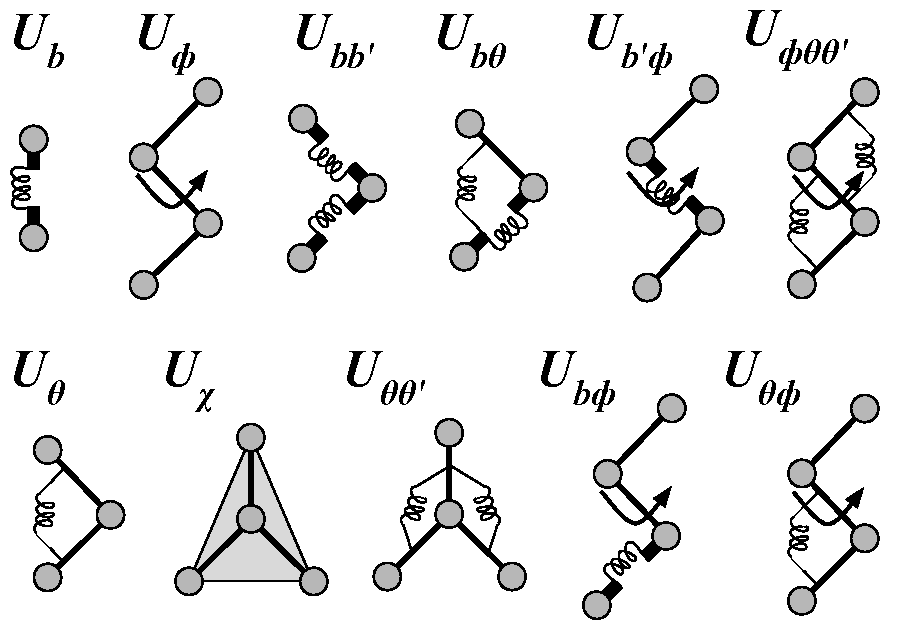
\includegraphics[width=15cm]{images/2_pcff_terms}
     \caption{Графическое пояснение к членам внутримолекулярной энергии уравнения \ref{pcff_eqn}.}
  \label{fig:2_pcff_terms}
\end{figure}

\textit{>>}

\subsection{Методы молекулярной динамики}

Определив модель молекулярной механики, можно применять различные методы для ее анализа; они включают в себя минимизацию энергии, моделирование молекулярной динамики, моделирование по методу Монте-Карло, а также различные более сложные методы, основанные на этих методах. Ключевым методом данной работы (а также, вероятно, наиболее часто используемым для изучения сложных молекулярных систем) является метод моделирования молекулярной динамики (МД) и его различных вариаций. Основная идея метода МД моделирования очень проста и основана на численном решении классических уравнений движения атомов в молекулярной системе на основе второго закона Ньютона:

\begin{equation}
    \frac{d^2 \overrightarrow{r_i}}{dt^2}= \overrightarrow{a}= \frac{\overrightarrow{F}}{m}= - \frac{1}{m_i} \nabla_i U(\textrm \{\vec{r_i}\})
\end{equation}
 
Численное решение обычно получается с помощью одной из схем интегрирования, такой как алгоритм Верле (velocity Verlet algorithm) \cite{swope_computer_1982}:

\begin{eqnarray}
    \overrightarrow{r}(t+\triangle t) = \overrightarrow{r}(t)+\overrightarrow{v}(t)\triangle t + \frac{1}{2} \overrightarrow{a}(t) \triangle t^2  \nonumber \\
    \overrightarrow{v}((t +\triangle t) =   \overrightarrow{v}(t) \frac{\overrightarrow{a}(t)+\overrightarrow{a}(t +\triangle t)}{2} \triangle (t)
\end{eqnarray}

Хотя основная идея, лежащая в основе МД-моделирования, на первый взгляд кажется довольно простой и понятной, ее обоснованность и интерпретация связаны с фундаментальными проблемами теоретической физики и математики на стыке механики, статистической физики и теории хаоса \cite{hoover_time_2001}. Одним из таких вопросов является связь между обратимыми во времени уравнениями Ньютона, используемыми для моделирования эволюции системы во времени, и эмпирическими необратимыми законами термодинамики, приводящими систему к состоянию, в котором энтропия максимальна.
    Другой набор вопросов и приближений, который имеет большое значение для практической реализации МД моделирования в реальных молекулярных системах, будет кратко обсужден ниже и включает использование периодических граничных условий, реализацию статистических ансамблей, динамику Ланжевена и диссипативных частиц, вычисления несвязанных взаимодействий, параллельная реализация МД алгоритмов.

\subsection{Периодические граничные условия}

Периодические граничные условия (ПГУ) - это метод, используемый для уменьшения влияния граничных эффектов на молекулярную систему во время моделирования и аппроксимации свойств объемных систем (таких как газы или жидкости) с помощью модели, состоящей из конечного набора молекул. Типичный случай применения периодических граничных условий - моделирование макромолекул в явном растворителе.
    В периодических граничных условиях ячейка моделирования окружена своими периодическими копиями во всех трех пространственных направлениях (см. Рисунок \ref{fig:p1_1:f11}), таким образом, эффективно образуя бесконечную кристаллическую структуру. Каждый атом, характеризуемый своими действительными координатами, также имеет координаты своих периодических образов. Распространенной формой учета частиц в периодических граничных условиях является соглашение о ближайшем образе, при котором каждый отдельный атом в системе взаимодействует с ближайшим к себе образом каждой частицы в системе.

\begin{figure} [h!]
    \centering
    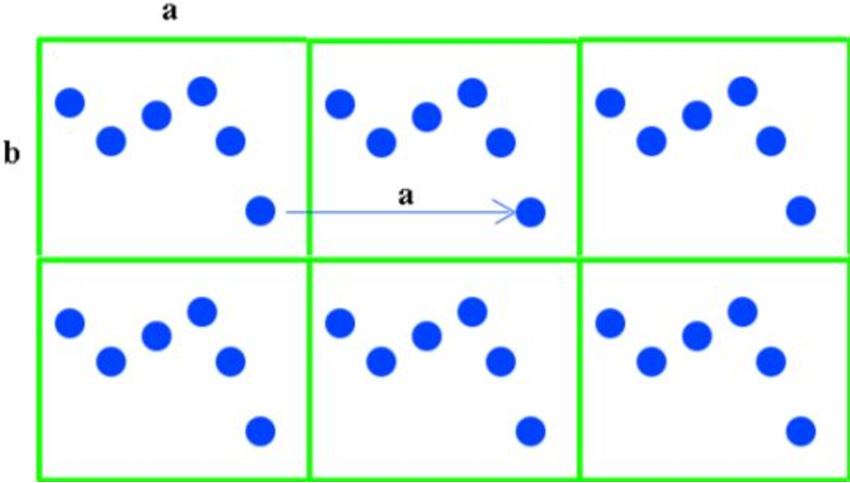
\includegraphics [width=\textwidth]{images/p1/part1_1_md/part1_1_md_f11.pdf}
    \caption[Иллюстрация периодических граничных условий]{Иллюстрация периодических граничных условий, используемых в МД моделировании. Кружками обозначены атомы и их периодические образы в соседних периодических ячейках.}
    \label{fig:p1_1:f11}
\end{figure}

ПГУ также используются в сочетании с методами учета электростатических взаимодействий на больших расстояния, такими как суммирование по Эвальду \cite{sagui_molecular_1999}. Поэтому полный электростатический заряд системы должен быть равен нулю, чтобы избежать проблем с расхождением значений полной электростатической энергии. Однако даже если система нейтральна, общий дипольный момент ячейки может приводить к некоторым искусственным энергетическим эффектам, похожим на пироэлектрические эффекты в полярных кристаллах.
Чтобы предотвратить артефакты связанные с ПГУ, размер ячейки моделирования должен быть достаточно большим, чтобы избежать таких нефизических эффектов. В том числе если размер ячейки слишком мал, макромолекула может взаимодействовать со своим собственным изображением в соседней ячейке, что эквивалентно взаимодействию молекулы с собой. Это может привести к нефизической динамике большинства макромолекул.

\subsection{Статистические ансамбли в МД моделировании}

Настоящие молекулярные системы никогда не изолированы от окружающей среды. Взаимодействие молекулярной системы с окружающей средой в плане обмена энергией, объемом и частицами с точки зрения статистической физики может быть описано в терминах статистических ансамблей \cite{landau_statistical_2000}. Ансамбль микросостояний молекулярной системы, связанной с внешним термостатом с постоянной температурой, называется каноническим ансамблем (или NVT-ансамблем), аналогично система под поршнем, связанная с термостатом, дает изобаро-изотермический ансамбль (или NPT -ансамбль).

    Поскольку базовые алгоритмы МД моделирования обеспечивают решение уравнений движения для изолированной системы (микроканонический ансамбль), обычно вводятся специальные алгоритмы, которые имитируют связь системы с внешним резервуаром энергии или объема \cite{frenkel_understanding_2002}. Цель таких алгоритмов - поддерживать правильные характеристики средней температуры (объема), в то же время обеспечивая правильную величину колебаний, которые зависят от внутренних свойств системы, таких как теплоемкость и сжимаемость.
    Среди алгоритмов термостатирования следующие алгоритмы нашли применение в современных кодах моделирования: термостат Берендсена \cite{berendsen_molecular_1984}, термостат Нозе-Гувера \cite{hoover_canonical_1985}, цепи Нозе-Гувера \cite{martyna_nose-hoover_1992}, термостат Андерсена \cite{andersen_molecular_1980}, термостат решкалирования скоростей \cite{bussi_canonical_2007}.
    
    Термостат Берендсена, будучи самым простым, полагается на масштабирование скоростей с коэффициентом $\lambda$  на каждом временном шаге:
\begin{equation}
   \lambda= \sqrt{\Big[1+\frac{\triangle t}{\tau_t} \Big\{\frac{T_0}{T}-1  \Big\} \Big]}
\end{equation}
    Влияние этого алгоритма на температуру заключается в том, что фактическая температура корректируется до эталонной температуры $T_0$ экспоненциальным образом:
\begin{equation}
    \frac{dT}{dt}= \frac{T_0 - T}{\tau}
\end{equation}
Однако термостат Берендсена имеет серьезные недостатки: во-первых, он не допускает колебаний температуры и, таким образом, не реализует правильный ансамбль, и, во-вторых, было показано, что процедура перемасштабирования скорости вызывает ``эффект летающего куба'' при моделировании системы в вакууме, когда энергия связанная с поступательным движением и вращением всей системы непрерывно растут, в то время как энергия высокочастотных основных мод истощается \cite{harvey_flying_1998,golo_dynamic_2002}.
    Формализм Нозе-Гувера - это подход, основанный на расширенном лагранжиане, содержащем дополнительные искусственные координаты и скорости, который приводит к детерминированной молекулярной динамике при постоянной температуре. Расширенный гамильтониан, первоначально предложенный Нозе \cite{nose_molecular_1984}, можно записать следующим образом:
\begin{equation}
    H_{Nose}= \sum_{i=1}^{N} \frac{\tilde {\mathbf p}_{i}^{2}}{2 m_i \tilde s^2} + U (\tilde r^N) + \frac{\tilde {\mathbf p}_{s}^{2}}{2Q} + g k T_0 ln(\tilde s)
\end{equation}
    где ${\mathbf p}_s$ и s - координаты расширенной переменной, Q - ее фиктивная масса, k - постоянная Больцмана, $T_0$-эталонная температура, g - параметр. Этот гамильтониан порождает микроканонический ансамбль из 6N + 2 степеней свободы. Переменные, присутствующие в этом гамильтониане, называются виртуальными переменными. Тем временем определяется набор реальных переменных, которые соотносятся с виртуальными переменными следующим образом:
\begin{eqnarray}
    {\mathbf r}= \tilde {\mathbf r} \\
    {\mathbf p}= \tilde {\mathbf p} /s \\
    s= \tilde s \\
    dt=d \tilde t / s
\end{eqnarray}
    и псевдогамильтониан может быть тогда задан как 
\begin{equation}
    H({\mathbf p},{\mathbf r})= \sum_{i=1}^{N} \frac{{\mathbf p}_{i}^{2}}{2m_i}+ U({\mathbf r}^N)
\label{pseudoH}
\end{equation}
Можно показать, что микроканонический ансамбль, сгенерированный путем решения уравнений движения для расширенной системы в виртуальных переменных, будет соответствовать канонической выборке реальных переменных согласно соответствующему псевдогамильтониану (\ref{pseudoH}), если параметр g = 3N и другие условия выполнены (см. ниже). Тепло передается в реальную систему и обратно от расширенной переменной колебательным образом, что приводит к почти периодическим колебаниям температуры. 
    Позже Нозе и Гувер показали, что соответствующие уравнения движения могут быть сформулированы в терминах реальных системных переменных, что дает уравнения движения Нозе-Гувера:
\begin{eqnarray}
    \ddot{{\mathbf r}_i} = \frac{{\mathbf F}_i}{m_i} - \frac{\xi \dot{{\mathbf r}_i}}{m_i} \nonumber \\
    \dot{\xi}= \frac{kg}{Q}(T(t)-T_0)
\end{eqnarray}

    Детальный теоретический анализ негамильтоновой динамики, генерируемой уравнениями Нозе-Гувера, показывает, что алгоритм генерирует правильное распределение только при наличии единственного интеграла движения, сохраняющегося во время динамики, обычно полной энергии расширенной системы, и никаких других интегралов движения \cite{frenkel_understanding_2002}. Исключением является сохранения полного импульса системы, если центр масс остается неподвижным.
    
    Данное утверждение также подразумевает, что динамика является эргодической, то есть усреднение по траектории эквивалентно усреднению по фазовому пространству. Однако было показано, что для небольших или жестких систем динамика неэргодична, и правильные распределения не генерируются. Чтобы решить эту проблему, Martyna et al. \cite{martyna_nose-hoover_1992} предложили схему, в которой термостат Нозе-Гувера соединен с другим термостатом или цепочкой термостатов.
    
    В подходе Андерсена к изотермическому моделированию система связана с термостатом с помощью стохастических импульсных сил, которые время от времени действуют на случайно выбранные частицы. В процессе столкновения частицы приобретают новые скорости согласно распределению Максвелла-Больцмана, соответствующие заданной температуре. Термостат Андерсена обеспечивает правильный статистический ансамбль, но делает динамику прерывистой из-за случайных столкновений.
    
    Термостат решкалирования скорости (Velocity rescale), предложенный Bussi et al. \cite{bussi_canonical_2007} представляет собой комбинацию термостата Берендсена со стохастическим членом, который обеспечивает правильное распределение кинетической энергии.
    
    
    Аналогично алгоритмам термостатирования существуют алгоритмы баростатирования, которые позволяют реализовать правильное целевое давление и NPT ансамбль. Схема баростатирования Берендсена \cite{berendsen_molecular_1984} позволяет быстро отрелаксировать систему до целевого давления и поддерживать его на протяжении всего моделирования. Алгоритм Берендсена изменяет масштаб координат и векторов ячейки моделирования на каждом шаге с помощью матрицы $\mu$ при заданном эталонном давлении $P_o$ следующим образом:
\begin{equation}
    \hat{\mu}_{ij}= \delta_{ij} - \frac{\triangle t}{3 \tau_p} \beta_{ij} \big\{P_{0ij}-P_{ij}(t)\big\}
\end{equation}
Где $\beta$ - изотермическая сжимаемость.
    Это приводит к экспоненциальной релаксации давления в соответствии с законом:
\begin{equation}
    \frac{dP}{dt}=\frac{P_0 -P(t)}{\tau_p}
\end{equation}
Как и в случае с термостатом, баростат Берендсена не полностью реализует NPT ансамбль и подавляет правильные флуктуации давления и объема, однако, если эти флуктуации не являются термодинамически значимыми, данный подход является простым и удобным методом поддержания постоянного давления в системе.

    Другой схемой поддержания давления, аналогичной термостату Нозе-Гувера, которая правильно реализует NPT ансамбль, является схема  Парринелло-Рамана \cite{parrinello_polymorphic_1981}.

\subsection{Ланжевеновская и диссипативная динамика частиц}
    Ланжевеновская (или стохастическая) динамика и диссипативная динамика частиц (ДДЧ) (dissipative particle dynamics) - это методы, которые позволяют имитировать влияние растворителя на динамику молекулярной системы посредством введения диссипативных и стохастических членов в уравнения движения. Взаимодействие диссипативных и стохастических сил не только изменяет динамику, но также может гарантировать правильные характеристики NVT ансамбля. В пределе небольшого воздействия (малая вязкость растворителя) эти методы также являются удобными алгоритмами для поддержания NVT ансамбля при моделировании методом МД.
    
    
    Стохастическая или скоростная динамика Ланжевена добавляет трение и шум к уравнениям движения Ньютона следующим образом:
\begin{equation}
   m_i \ddot{{\mathbf r}}={\mathbf F}_i - m_i \xi_i \dot{{\mathbf r}} + \hat{{\mathbf r}_i}
   \label{eq:p1:langevin}
\end{equation}
    где $\xi_i$ - постоянная трения, а $\hat{r_i}(t)$ - это шумовой процесс с корреляционной функцией
\begin{equation}
   \big  \langle \hat{r}_{i}^{\alpha}(t)\hat{r}_{i}^{\beta}(t+s) \big \rangle = 2m_i \xi_i kT \delta(s) \delta_{ij} \delta_{\alpha\beta}
   \label{eq:p1:lang_proc}
\end{equation}
т.е. он нескоррелирован для разных частиц, разных компонентов и разного времени. Формальный вывод уравнения Ланжевена посредством редукции быстрых степеней свободы и их аппроксимации двумя последними членами уравнения (\ref{eq:p1:langevin}) основан на технике проекционного оператора, введенной Мори и Цванцигом \cite{zwanzig_nonequilibrium_2001}. В остальном члены, отвечающие за трение и стохастический процесс, имеют интуитивно понятный физический смысл: первая представляет собой диссипативную силу, вызываемую трением с растворителем, вторая - своего рода движущую силу, которая вызывается ``ударами'' окружающих частиц растворителя.

Случайное трение и стохастические силы не сохраняют ни импульс, ни энергию системы. Под действием силы трения энергия отводится из системы, в то время как стохастический процесс может закачивать энергию в систему, поэтому динамика и выборка больше не соответствуют микроканоническому ансамблю, в то время как энергия системы флуктуирует, что напоминает канонический ансамбль NVT. Кроме того, можно показать, что для реализации распределения Больцмана в стохастической динамике трение и стохастические силы должны быть связаны через уравнение (\ref{eq:p1:lang_proc}).
        
Хотя метод Ланжевена привлекателен для жидкостных систем, где структура растворителя не важна, или как алгоритм для строгой реализации ансамбля NVT, он не дает правильной гидродинамики, поскольку случайные силы и силы трения не сохраняют импульс системы. Чтобы преодолеть эту проблему, но при этом сохранить положительные черты стохастической динамики, метод диссипативной динамики частиц (ДДЧ) (dissipative particle dynamics) был первоначально разработан Хугербрюгге и Кольманом для мезоскопического моделирования простых и сложных жидкостей \cite{hoogerbrugge_simulating_1992}. В ДДЧ сила, действующая на каждую частицу, состоит из трех членов \cite{moeendarbary_dissipative_2009}:
\begin{equation}
    {\mathbf F}_i= \sum_{j \neq i} ({\mathbf F}_{ij}^{C} + {\mathbf F}_{ij}^{D} +{\mathbf F}_{ij}^{R})
\end{equation}
консервативная сила, диссипативная сила и случайная сила, соответственно. В то время, как консервативная сила является обычной парной силой, диссипативная и случайная силы определяются следующим образом:
\begin{equation}
   {\mathbf F}_{ij}^{D} = -\gamma \omega_D (r_{ij})({\mathbf n}_{ij} \cdot {\mathbf v}_{ij}) {\mathbf n}_{ij}
\end{equation}
\begin{equation}
   {\mathbf F}_{ij}^{R}= \sigma \omega_R (r_{ij}) \zeta_{ij} {\mathbf n}_{ij}
\end{equation}
где $r_{ij}= |{\mathbf r}_i -{\mathbf r}_j|$j, ${\mathbf n}_{ij}= {\mathbf r}_{ij}/|{\mathbf r}_{ij}|$, $\gamma$ и $\sigma$ - скалярные параметры, представляющие силу трения и случайную силу. $\omega_D$ и $\omega_R$ - весовые коэффициенты, которые варьируются от 0 до 1 и исчезают выше радиуса отсечки $R_c$. $\zeta_{ij}$ - представляет собой гауссовский белый шум со следующими свойствами:
\begin{equation}
   \big\langle \zeta_{ij}(t) \big\rangle = 0, \zeta_{ij}=\zeta_{ji}
\end{equation}
\begin{equation}
    \big\langle \zeta_{ij}(t) \zeta_{i' j'}(t') \big \rangle= \big( \delta_{ii'}\delta_{jj'}+\delta_{ij'}\delta_{i'j} \big) \delta(t-t')
\end{equation}
Замечательной особенностью уравнений ДДЧ в отличие от динамики Ланжевена является то, что
диссипативные и случайные силы зависят только от относительного положения и скорости
частицы и действуют по векторам, соединяющим пары частиц. Это в сочетании с
симметрией индексов обеспечивает выполнение третьего закона Ньютона и сохранение количества движения. Далее можно показать, что уравнения ДДЧ описывают
системы в ансамбле NVT при $\sigma^2 = 2\gamma kT$. Выбор одной весовой функции может
быть произвольным, однако можно показать, что обе функции должны быть связаны как
$\omega_D (r) = (\omega_R (r))^2$.
Типичный выбор для этой функции:
\begin{equation}
    \omega (r)= \Bigg\{ 2 \bigg(1- \frac{r}{R_c}    \bigg), r \leq R_c  ;   0, r > R_c\Bigg\}
\end{equation}
ДДЧ в основном применяется как метод мезоскопического моделирования, где частицы ДДЧ представляют собой целые молекулы или области жидкости, а не отдельные атомы. Однако трение и случайные члены могут также использоваться в атомистическом моделировании для моделирования влияния растворителя и реализации ансамбля NVT. Преимуществами термостата ДДЧ перед термостатом Ланжевена является сохранение импульса и малый радиус взаимодействий ДДЧ, оба фактора способствуют крупномасштабным конформационным переходам в молекулярной системе, если они должны произойти.

\subsection{Расчет невалентных взаимодействий}
    Вычисление невалентных взаимодействий и особенно кулоновских взаимодействий - одна из задач МД моделирования. Важной отличительной чертой электростатических взаимодействий является их медленный затухающий характер $(\sim 1/r)$, что, строго говоря, делает некорректным обрезку электростатического взаимодействия на некотором расстоянии во время вычисления сил и энергии при моделировании. В трехмерной объемной системе энергия взаимодействия точечной частицы с окружающей средой, характеризуемой плотностью заряда $\rho (r)$, была бы выражена интегралом:
\begin{equation}
   E= \iiint \frac{\rho (\vec{r})}{|\vec{r}- \vec{r}_0|} d^3 \vec{r}
\end{equation}
    который может сходиться только условно. Таким образом, необходимо соблюдать особую осторожность при расчете электростатических взаимодействий в моделировании МД. Было показано, что при простой обрезке кулоновских взаимодействий могут возникать серьезные артефакты, особенно при моделировании систем зарядов, начиная от шума и нестабильности при моделировании и заканчивая неблагоприятным воздействием на молекулярный порядок \cite{sagui_molecular_1999}.
    Если изучаемая система не является периодической (т.е. не используются периодические граничные условия), единственной альтернативой полному расчету электростатических взаимодействий (что для больших систем является недопустимо дорогостоящим, поскольку масштабируется как $\sim N^2)$ является их обрезка на некотором расстоянии Rc. Однако необходимо обосновать отсутствие серьезных побочных эффектов в таком случае. Наиболее распространенные ошибки могут возникать из-за: (i) отсутствия непрерывности силы, особенно при образовании нескомпенсированных зарядов на длине радиуса обрезания, приводящего к алгоритмическому шуму и тепловыделению, (ii) для заряженных систем и систем с внутренней периодичностью энергия и поведение системы могут зависеть от радиуса обрезания причудливым образом.
    
    В системах, которые используют периодические граничные условия, может использоваться альтернативная более надежная стратегия суммирования электростатических взаимодействий, она основана на методе суммирования Эвальда и родственных алгоритмах PME (particle mesh Ewald) и PPPM (particle-particle particle-mesh Ewald), основанные на интерполяции функций по значениям в узлах сеток \cite{frenkel_understanding_2002}. Идея суммирования по Эвальду состоит в том, чтобы заменить бесконечную медленно сходящуюся сумму электростатического взаимодействия данного набора частиц и всех их периодических образов двумя быстро сходящимися суммами, одна в прямом, а другая - в обратном пространстве. Рассмотрим представление набора точечных зарядов, дополненных гауссовыми функциями экранирования и их обратными функциями на рисунке \ref{fig:p1_1:f12}.

\begin{figure} [h!]
    \centering
    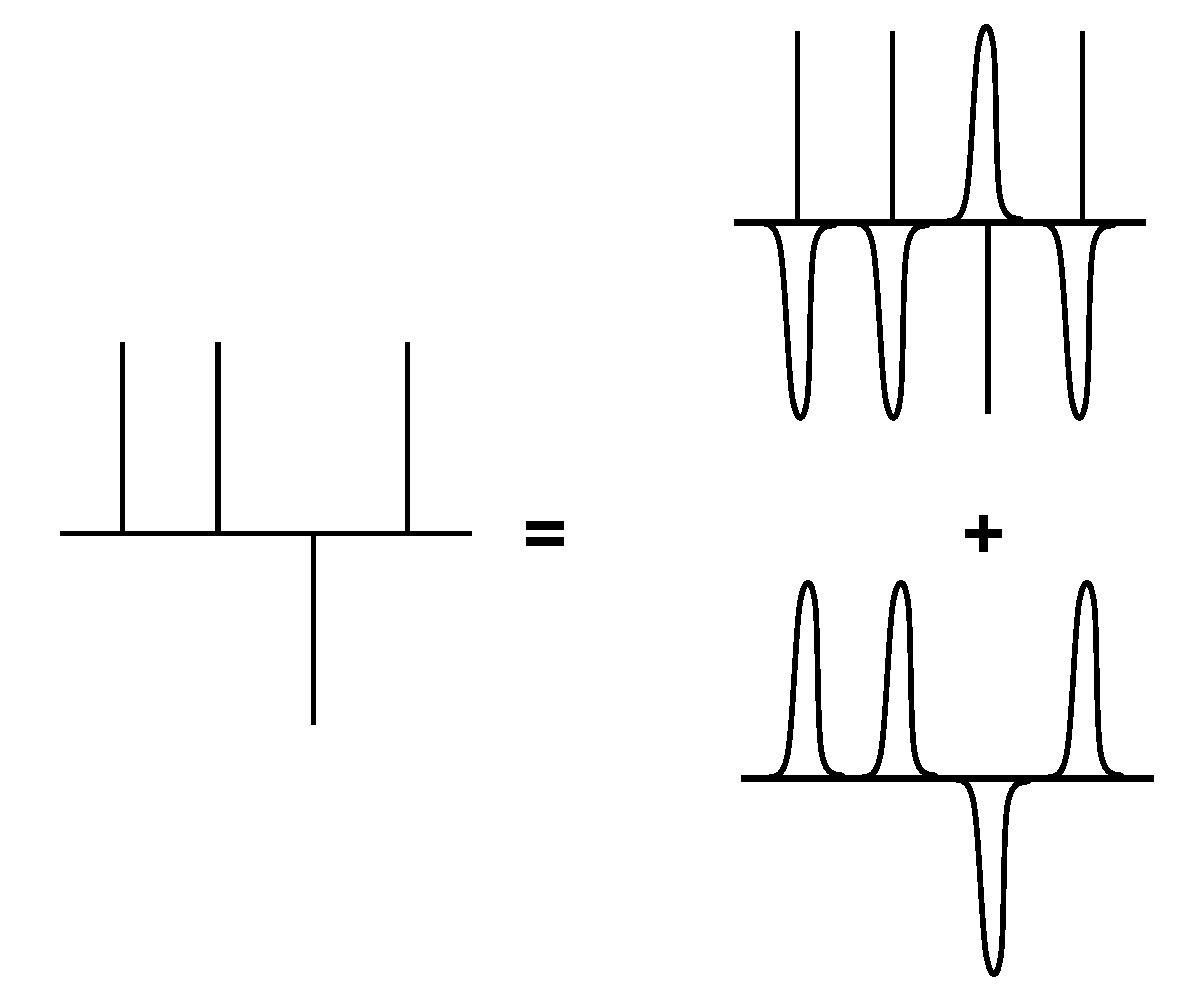
\includegraphics [width=\textwidth]{images/p1/part1_1_md/part1_1_md_f12.pdf}
    \caption{Схематическое изображение разложения заряда, используемого в суммировании по Эвальду.}
    \label{fig:p1_1:f12}
\end{figure}

    Гауссовские экранирующие функции имеют вид:

\begin{equation}
    \rho_{Gauss}(r)= -q_i(\alpha/\pi)^{3/2} exp(-\alpha r^2)
\end{equation}
    Можно показать, что в этом случае полный электростатический потенциал может быть выражен как сумма потенциалов обеих подсистем, представленных на рисунке \ref{fig:p1_1:f12}, за вычетом члена энергии самовзаимодействия. Электростатический потенциал экранированных точечных зарядов быстро спадает и может быть суммирован в прямом пространстве, в то время как потенциал компенсирующей подсистемы (плавно меняющиеся периодические гауссианы) можно легко вычислить в обратном пространстве Фурье на основе решения уравнения Пуассона. Результирующая полная энергия системы может быть записана следующим образом:
\begin{equation}
    U= \frac{1}{2} \sum_{i \neq j}^{N} \frac{q_i q_j \erfc{(\sqrt{\alpha}r_{ij})}}{r_{ij}} + \frac{1}{2V} \sum_{k \neq 0}\frac{4 \pi}{k^2} |\rho ({\mathbf k})|^2 exp(-k^2 / 4\alpha) - (\alpha/ \pi)^{1/2} \sum_{i=1}^{N} q_{i}^{2}
\end{equation}
    где $\rho ({\mathbf k}) \equiv \sum_{i=1}^{N} q_i exp(i{\mathbf k} \cdot {\mathbf r}_i)$, V - объем периодической ячейки.

    Однако сумма Эвальда требует больших вычислительных ресурсов для больших систем с порядком масштабирования  $O(N^{3/2})$ и остается дорогостоящей по сравнению с традиционными схемами обрезки взаимодействий. Чтобы решить эту проблему, были разработаны подходы на основе интерполяционных сеток, все они пытаются ускорить решение уравнения Пуассона в периодических граничных условиях, используя преимущества быстрого преобразования Фурье (БПФ) для вычисления дискретных преобразований Фурье \cite{sagui_molecular_1999}. Эти методы могут масштабироваться как $O(N log (N))$.
    Методы суммирования, подобные суммированию по Эвальду, могут вычислять электростатическую энергию в периодической системе с заданной точностью. Их использование привело к значительному повышению стабильности при моделировании биомолекул. Однако, некоторые фундаментальные проблемы моделирования все еще существуют и могут привести к артефактам во время моделирования \cite{sagui_molecular_1999}. Смит и Петтитт \cite{smith_ewald_1996,smith_presence_1997} изучали динамические артефакты, вызванные суммированием по Эвальду. Они сосредоточились на вопросе о величине энергетических барьеров при свободном вращении диполей в системах с периодичностью (наличием дальнего порядка). Представьте себе единственный идеальный диполь в начале элементарной ячейки, который затем периодически воспроизводится в соседних ячейках. Потенциальная энергия системы будет зависеть от ориентации диполя, что не подходит для исследования растворов биомолекул. Однако Смит и Петтитт показали, что вращательные барьеры незначительны для дипольных молекул в растворителях с высокой диэлектрической проницаемостью при комнатной температуре с типичными размерами ячейки моделирования. Для моделирования в растворителях с низкой диэлектрической проницаемостью или в вакууме отсутствие артефактов не может быть гарантированно.






% \subsection{Методы молекулярной динамики}
% Задача молекулярной динамики фактически заключается в решении классических уравнений движения для системы с заданным гамильтонианом. Решение уравнений движения реализуется численно с помощью разностных схем таких, как алгоритм Верле или Лип-Фрог алгоритм. Важной особенностью ``хороших'' алгоритмов является обратимость во времени и сохранение объёма фазового пространства. Известно также, что алгоритм Верле обладает ``теневой'' характеристикой, то есть точки траектории, получаемые посредством этого алгоритма, точно соответствуют (конечно, за исключением ошибки численного округления) некоторой ``теневой траектории'' механической системы, которая однако не проходит, через точку с начальными условиями. Иными словами, алгоритм Верле генерирует траекторию, которая соответствует экстремуму действия для некоторой ``теневой траектории'' (\cite{Frenkel} разд. 4.3.5).

% Для решения проблемы поверхностных эффектов в методе МД применяют периодические граничные условия. Особое внимание в последнее время обращается на тот факт, что при использовании периодических условий необходимо использовать решёточные алгоритмы для учёта дальнодействующих взаимодействий, таких как электростатические, поскольку обрезание зарядовых взаимодействий может приводить к артефактам моделирования. На данный момент хорошо разработаны достаточно быстрые решёточные алгоритмы учёта электростатики такие, как методы PME и PPPM.

% Отдельной проблемой является задание ансамблей в методе молекулярной динамики. Для задания распределения по температуре существует два принципиальных подхода: стохастическая и негамильтонова динамика. В стохастическом подходе в уравнения движения вводятся случайные члены (например, такие как в уравнении Ланжевена), которые позволяют привести статистическое распределение точек МД траектории к каноническому ансамблю. Подход негамильтоновой динамики был предложен Гувером \cite{Hoover}, он разработал такую модификацию уравнений движения, в которой предельным для точек фазового пространства является каноническое распределение. Однако в оригинальном алгоритме Нозе-Гувера были найдены проблемы при некоторых условиях, и на данный момент наиболее надёжным считается алгоритм цепей Нозе-Гувера.




%\section{Методы расчета свободной энергии в молекулярном моделировании}
%\section{Методы расчета свободной энергии взаимодействия с растворителем в молекулярном моделировании}

Предположим, что молекулярная система характеризуется некоторым Гамильтонианом, зависящим от параметра: $H(\lambda)$. \textit{Будем говорить, что каждому значению $\lambda$ соответствует некоторое $\lambda$-состояние системы.} Каким образом возможно рассчитать разницу в свободной энергии меду двумя $\lambda$-состояниями?\\

Начиная с 1960-х годов для практической реализации в численных экспериментах широкое применение получили такие методы, как \textit{метод термодинамического интегрирования}, \textit{метод возмущения свободной энергии}, \textit{метод Беннетта}. С появлением работ  Джарзинского, Крукса, Шёртса и др. \cite{jarzinski,crooks,stanford_ben} выявилась более глубокая связь между этими методами. Соотношения неравновесной статистической физики, выведенные Джарзинским (Jarzinsky equality) и Круксом (transient fluctuation theorem) предлагают более общий подход к решению задачи отыскания свободной энергии через неравновесные процессы. При этом, упомянутые ранее методы являются частными случаями в этом общем подходе, но могут также быть получены независимыми способами.
В данной работе нам будут интересны эти три метода, так как они имеют широкое практическое применение.
\subsection{Метод термодинамического интегрирования}
Метод ТИ может быть получен из простых соображений. Свободная энергия Гиббса системы задаётся в общем случае выражением \ref{gibbsFE}.
\begin{equation}
G=-kT\ln\int \exp\left(-\frac{H(V,\vec{p},\vec{q},\lambda)+PV}{kT}\right)d\vec{p}d\vec{q}dV
\label{gibbsFE}
\end{equation}
Для метода ТИ основным является равенство \ref{TI_equal}.
\begin{equation}
\frac{\partial G}{\partial \lambda}=\left\langle \frac{\partial H}{\partial \lambda} \right\rangle
\label{TI_equal}
\end{equation}
И разница свободной энергии между разными $\lambda$-состояниями даётся выражением \ref{TI}.
\begin{equation}
\Delta G=\int \frac{\partial G}{\partial \lambda} d\lambda
\label{TI}
\end{equation}

Метод достаточно эффективен и часто применяется. Однако, необходимость интегрирования функции $\frac{\partial G}{\partial \lambda}$ требует достаточно большого количества вычислений и вносит дополнительную ошибку численного интегрирования, которую трудно оценить при ограниченном наборе известных значений функции.

\subsection{Метод возмущения свободной энергии} 
В методе возмущения свободной энергии (Free energy perturbation - FEP) разница свободной энергии между разными $\lambda$-состояниями может быть записана в виде \ref{fep_equal}, что и определяет метод отыскания разницы свободной энергии между двумя состояниями.
\begin{equation}
\Delta G=-kT \ln{\frac{\int dV\vec{p}d\vec{q}\exp \left \{ -\frac{H(V,\vec{p},\vec{q},\lambda_1)+PV}{kT} \right \}}{\int dV\vec{p}d\vec{q}\exp \left \{ -\frac{H(V,\vec{p},\vec{q},\lambda_0)+PV}{kT} \right \}}}=-kT
 \ln{<\exp{\frac{H_0-H_1}{kT}}>_0}
\label{fep_equal}	
\end{equation}
где $H_0=H(V,\vec{p},\vec{q},\lambda_0)$, $H_1=H(V,\vec{p},\vec{q},\lambda_1)$, усреднение ведётся по NPT-ансамблю соответствующему состоянию системы с $\lambda=\lambda_0$.

\subsection{Метод Беннетта}
Метод Беннетта (Bennett acceptance ratio method) позволяет наиболее эффективным образом комбинировать данные, получаемые при прямом и обратном процессе. Иными словами, мы переводим систему из состояния с $\lambda=\lambda_0$ в состояние с $\lambda=\lambda_1$ и при этом получаем некоторое значение работы $W_F$. Однако возможен и обратный процесс перевода системы из состояния $\lambda_1$ в состояние $\lambda_0$ с работой $W_R$. В 1976 году метод был предложен Беннеттом \cite{bennet} как обобщение метода FEP. Однако в настоящее время стало ясно, что таким образом можно обобщить практически любые методы расчёта свободной энергии. Этот \textit{обобщённый метод Беннетта} основывается на соотношениях Крукса и позволяет построить наилучшую статистику (оценочную функцию максимального правдоподобия) для оценки значения свободной энергии по наборам параметров $W_F$ и $W_R$ (см. \cite{stanford_ben}).\\

В простейшем случае как обобщение метода FEP метод Беннета (оригинальная работа \cite{bennet}, 1976 год) имеет следующий вид.
Итак, допустим, что у нас есть набор работ по бесконечно быстрой трансформации системы из состояния $\lambda_0$ в состояние $\lambda_1$ - ${W_F}$, и обратно - ${W_R}$. Метод Беннета задаёт оценочную функцию, которая определяет значение разницы свободной энергии с минимальной дисперсией среди всех оценочных функций.
Оценочная функция задаётся неявно, как решение уравнения \ref{beneq} по параметру $C$.

\begin{equation}
\label{beneq}
\sum _m^{N_R} f(W_R^m+C)=\sum _n^{N_F} f(W_F^n-C)
\end{equation}
В уравнении (\ref{beneq}) $f$-функция Ферми-Дирака:
$$
f(x)\equiv \frac{1}{1+\exp{\beta x}}
$$
$N_F$ и $N_R$ - соответственно количество полученных замеров в прямом и обратном направлениях, $\beta=1/kT$. Можно показать, что наилучший результат всегда достигается при $N_F\approx N_R$. Более того, метод Беннета имеет преимущество перед простым методом FEP. Так, более эффективным является осуществление выборки значений работы в прямом и обратном направлениях, и затем применение метода Беннета, чем осуществление в два раза большей выборки в одном направлении и применении метода FEP.

\subsection{Методы расширенных ансамблей}
Кроме трёх вышеприведённых методов развиваются и более современные методы расширенных ансамблей. В этих методах происходит одновременное моделирование систем при различных значениях параметра $\lambda$ и между этими состояниями осуществляются переходы, как в методе Монте-Карло. Хорошим примером адаптивного метода расширенных ансамблей является работа \cite{lyubartsev_2004}. Однако, на данный момент программное обеспечение, реализующее такие методы, мало распространено.

%Методы расчета молекулярных поверхностей
\section{Методы расчета поверхностей в молекулярном моделировании} \label{part1_3_sasa}
\textit{Раздел \ref{part1_3_sasa} изложен согласно кандидатской диссертации автора \cite{shaytan_thesis_kfmn_2010} << }
Поверхность доступная растворителю (ПДР) (solvent accessible surface area (SASA)) -- это поверхность биомолекулы, которая доступна растворителю. Обычно ПДР выражают с квадратных ангстремах. ПДР была впервые описана Ли и Ричардсом\cite{lee_richards} и иногда называется молекулярной поверхностью Ли-Ричардса, она определяется как поверхность которую описывает центр пробной сферы при ``обкатывании'' сферы вокруг молекулы. Размер сферы обычно берётся порядка размера молекулы воды. В этом плане ПДР можно воспринимать, как расширенную поверхность Ван-дер-Ваальса.

Кроме ПДР широкое распространение получила поверхность Коннолли, которая представляет собой как бы полость, которая формируется в растворителе при помещении в него молекулы. Коннолли разработал также полуаналитический метод расчёта такой поверхности \cite{connolly_1983}.

На Рис. \ref{f:2_surf} изображены поверхности доступные растворителю и молекулярные поверхности Коннолли для модельной системы.

\begin{figure}[htbp]
   \centering
   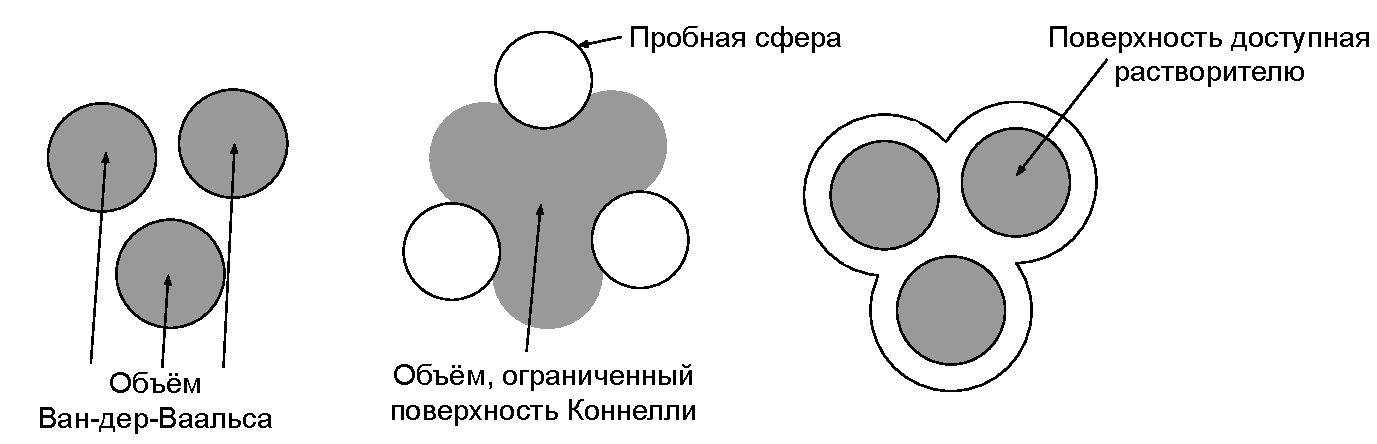
\includegraphics[width=15cm]{images/2_surf}
      \caption{Пояснения к определению поверхности доступной растворителю и поверхности Коннолли.}
   \label{f:2_surf}
\end{figure}
\textit{>>}

%\section{Методы моделирования ДНК в динуклеотидном приближении}
\section{Методы моделирования ДНК в динуклеотидном приближении}

Описание конформации ДНК в виде набора геометрических параметров, определяющих взаимное расположение соседних нуклеотидных пар относительно друг друга, может использоваться как для исследования структуры ДНК, так и для создания физических моделей гибкости ДНК. Последние могут быть встроены в алгоритмы интегративного моделирования ДНК и ДНК-белковых комплексов. В данном разделе излагаются представления о  параметрах геометрии ДНК, эмпирических силовых полях для описания энергии изгиба ДНК в динуклеотидном приближении, а также программные продукты и методы моделирования, включая разработки научной группы автора.

\subsection{Описание геометрии ДНК}
Планарность азотистых оснований нуклеотидов и относительная планарность комплементарных пар оснований в двухцепочечной спирали ДНК позволяет применить для описания их взаимного расположения математический формализм, в котором основания или пары оснований представлены в виде плоских элементов с двумя уникальными гранями, отличимыми друг от друга из-за асимметрии оснований (см. Рис. \ref{fig:p1:DNA_param}). Разработке данных подходов способствовали работы Р. Дикерсона \cite{dickerson_definitions_1989}, В.Б. Журкина, В.И.Иванова,  В.П.Лысова \cite{zhurkin_anisotropic_1979}, В. Олсон, К. Лу \cite{lu_3dna_2003}, М. Эль Хассана, К. Калладайна \cite{el_hassan_assessment_1995} и др. Ниже сформулируем принятые на сегодняшний день подходы и алгоритмы.

Каждое азотистое основание (см. Рис. \ref{fig:p1:DNA_param}б) можно представить в виде твердого тела (при изображении обычно используются плоские прямоугольные параллелепипеды) и связанной с этим твердым телом системы отсчета. В 1999 на семинаре в Цукубе были приняты (а позднее утверждены совместной комиссией по биохимической номенклатуре Международного союза биохимии и молекулярной биологии и Международного союза теоретической и прикладной химии  (JCBN)) стандарты эталонной геометрии (расположения атомов) в идеализированных азотистых основания нуклеиновых кислот и их идеализированных Уотсон-Криковских парах \cite{olson_standard_2001}. Данные эталонной геометрии заданы в виде координат атомов относительно стандартной системы отсчета введенной для Уотсон-Криковских пар. При анализе структуры ДНК проводится совмещение эталонного основания или пары оснований с реальными по методу минимизации среднеквадратичного отклонения атомов (RMSD), таким образом каждому реальному основанию можно сопоставить, связанную с ним систему координат (см. Рис. \ref{fig:p1:DNA_param}в). В стандартной системе отсчета ось Z перпендикулярна плоскости основания и в структуре В-ДНК совпадает с направлением 5'-3' цепи ДНК для левого основания на Рис. \ref{fig:p1:DNA_param}в, ось Y параллельна линии соединяющей C1' атомы нуклеотидов, ось X направлена в сторону большой бороздки ДНК и совпадает с осью псевдосимметрии идеальной Уотсон-Криковской пары. Таким образом, в силу наличия оси псевдосимметрии эталонные координаты необходимо задать для оснований, когда они находятся в левом положении на Рис. \ref{fig:p1:DNA_param}в, координаты для их положения с правой стороны могут быть получены путем преобразования симметрии.

Определив положения систем отсчета, связанных с основаниями или парами оснований, можно ставить задачу о вычислении геометрических параметров взаимного расположения твердых тел, характеризуемыми этими системами отсчета. Из геометрии известно, что для описания взаимного расположения двух твердых тел относительно друг друга, необходимо шесть параметров, три из которых описывают поступательные степени свободы, а три вращательные. Номенклатура таких параметров была утверждена в 1988 году и носит название ``Кембриджского согласия'' (Cambridge Accord) \cite{dickerson_definitions_1989}.
Поступательные степени свободы для взаимного расположения оснований относительно друг друга носят названия Shear, Stretch, Stagger для смешения по осям X, Y, Z, соответственно (Рис. \ref{fig:p1:DNA_param}д). В случае определения этих параметров для Уотсон-Криковской пары M-N, по соглашению, систему координат основания N предварительно вращают вокруг оси X на 180 градусов. Вследствие этого, если рассматривать ту же самую пару как пару N-M, угловой параметр Buckle, обсуждаемый далее, поменяет знак на противоположный. Также при рассмотрении Уотсон-Криковской пары в обратном направлении (N-M вместо M-N) поменяет свой знак параметр Shear, но не параметры Stretch и Stagger. В случае рассмотрения Хугстиновских пар приняты другие правила, которые рассматривать здесь не будем.

Аналогично можно ввести параметры взаимного расположения пар оснований вдоль цепи ДНК, они носят название Shift, Slide, Rise для смещений вдоль осей X, Y, Z, соответственно. При рассмотрении двухцепочечной B-формы ДНК для вычисления данных параметров нам необходимо выбрать направление одной из цепей ДНК в качестве референсного, которое будет задавать направление последовательного рассмотрения пар оснований для вычисления параметров их взаимного расположения. При вычислении параметров в обратном направлении (в качестве референсной цепи задается комплиментарная цепь) знак параметра Shift поменяется на противоположный, а параметры Slide и Rise не изменят знака.

Вычисление параметров вращения оснований и пар оснований относительно друг друга представляет собой более сложную задачу, поскольку в отличие от преобразований смещения в трехмерном пространстве группа преобразований вращения являет некоммутативной, то есть зависит от последовательности применения операций вращения. Так в механике для описания вращения твердых тел зачастую используется углы Эйлера или матрицы поворота вокруг осей системы координат. Однако преобразования описываемые данными углами необходимо выполнять в определенной последовательности, конечный результат сложным образом зависит от всех трех углов. В случае описания взаимного расположения оснований ДНК таким образом углы Эйлера будут иметь трудно интерпретируемый физический смысл. Отдельной проблемой является то, что при изменении направления рассмотрения преобразований (например, M-N  вместо N-M или рассмотрении динуклеотидных переходов вдоль по одной и другой цепи ДНК) численные значения параметров вращения будут отличаться. Данная проблема была очевидна с конца 1970-ых годов (в 1981 году была установлена первая кристаллическая структура ДНК - додекамер Дрю-Дикерсона\cite{drew_structure_1981}), обсуждалась на встрече 1988 года в Кембридже (``Cambridge Accord'').  Для разрешения данной проблемы был сформулирован ряд подходов, которые для определения и вычисления параметров вращения оснований ДНК вводят понятие дополнительной системы отсчета, находящейся по середине между рассматриваемыми системами отсчета (см. напр. работу 1979 года В.Б. Журкина и др. \cite{zhurkin_anisotropic_1979}). Используя дополнительную систему отсчета можно сформулировать определение параметров вращения, которые будут независимы от направления рассмотрения преобразования.  Наиболее используемый подход был предложен Эль Хассаном и Калладайном и описан в статьях \cite{el_hassan_assessment_1995,lu_structure_1997}. Рассмотрим этот подход на примере расчета динуклеотидных параметров вращения Twist, Roll, Tilt (Рис. \ref{fig:p1:DNA_param}е), расширение данного подхода на параметры вращения оснований относительно друг друга Buckle, Propeller, Opening может быть произведено по аналогии. 

Для вычисления углов Twist, Roll и Tilt вводится система отсчета (``mid-step reference frame''), находящаяся по середине межу системами отсчета, связанными с последовательными парами оснований (см. Рис. \ref{fig:p1:DNA_param}г). Для преодоления проблемы некоммутативности операций вращения используется следующий прием. Вращение систем отчета друг относительно друга может быть представлено как вращение вокруг оси Z (Twist) на угол $\Omega$, а затем отклонение оси Z на некоторый угол $\Gamma$ вокруг какой-либо оси перпендикулярной оси Z (называемой остью RollTilt). В случае работы относительно промежуточной системы отчета (``mid-step reference frame'') процедура разлагается на поворот верхнего основания на угол $\Omega/2$ и угол $\Gamma/2$, а нижнего на угол $-\Omega/2$ и угол $-\Gamma/2$, относительно оси RollTilt, положение которой задается углом $\phi$ относительно оси Y промежуточной системы отсчета. Углы Roll ($\rho$) и Tilt ($\tau$) определяются векторным разложением по формулам:
\begin{eqnarray}
 \rho=\Gamma \cos(\phi)\\
 \tau=\Gamma \sin(\phi)
\end{eqnarray}
Позитивный Roll в А/B и W-формах ДНК соответствует открытию малой бороздки, знак параметра Tilt зависит от направления рассмотрения ДНК. Более подробное определение методов расчета параметров в современной реализации программы 3DNA может быть найдено в \cite{lu_structure_1997}.

Можно показать, что соответствующие процедуры позволяют определить схему, которая с точностью до знака дает одинаковые значения параметров при рассмотрении ДНК как в прямом, так и в обратном направлениях.
Важной особенностью данного подхода является то, что структура ДНК может быть однозначно восстановлена по наборам рассчитанных параметров. Таким образом, можно проводить конвертацию атомистических структур в пространство параметров оснований ДНК и обратно, а также генерировать структуры с измененной последовательностью, но идентичной геометрией. 


\begin{figure}[H] 
  \center
  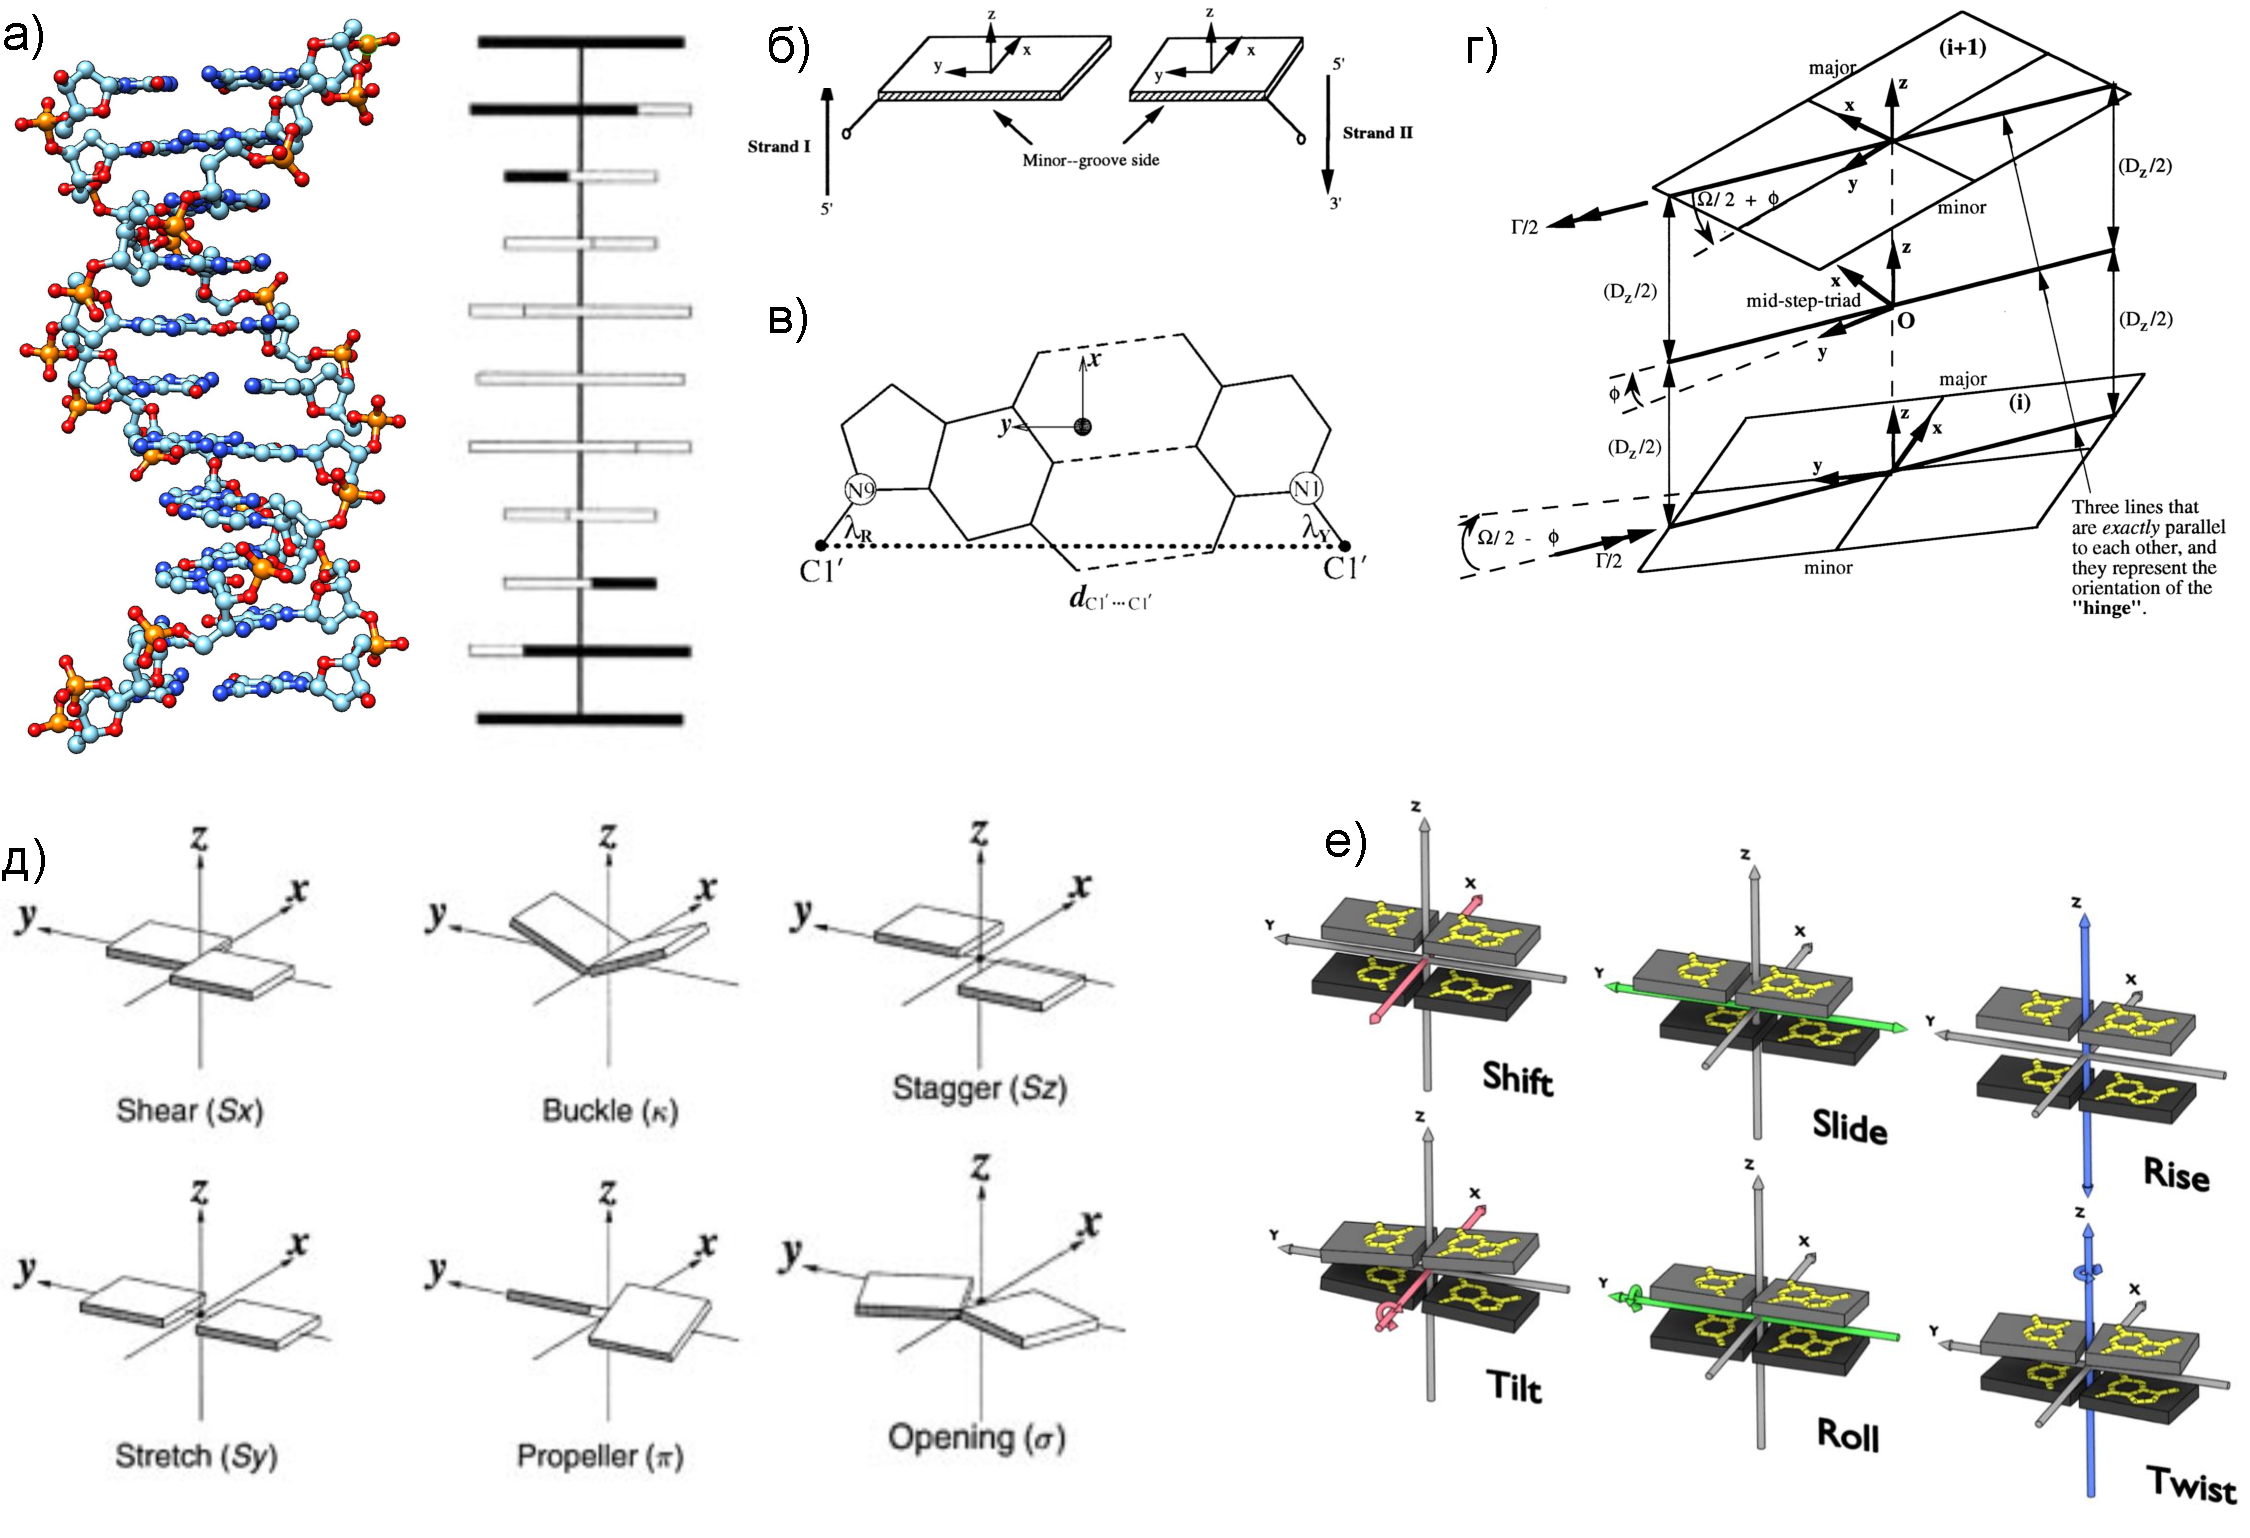
\includegraphics [width=\textwidth] {images/p1/DNA_param}
  \caption[Описание геометрии ДНК в виде геометрических параметров]{Описание геометрии ДНК в виде геометрических параметров. a) Атомистическое представление B-формы ДНК и представление в виде диаграммы по принципам Калладайна и Дрю \cite{calladine_understanding_2004}; б) представление пары оснований в виде параллелепипедов и связанные с ними системы координат \cite{el_hassan_assessment_1995}, в) система координат и ее расположение относительно пары оснований \cite{olson_standard_2001}, г) иллюстрация введения промежуточной системы отсчета между парами оснований для расчета параметров вращения  \cite{el_hassan_assessment_1995}, д) параметры взаимного расположения оснований в паре оснований \cite{lu_3dna_2003}, е) параметры взаимного расположения пар оснований относительно друг друга вдоль ДНК.} 
  \label{fig:p1:DNA_param}
\end{figure}

\subsection{Эмпирические константы жесткости изгиба ДНК}
Возможность задания общей конформации ДНК в виде набора 12 параметров, определяющих взаимное расположение азотистых оснований, позволяет поставить вопрос о возможности задания некоторого силового поля, способного описывать энергию различных конформаций двухцепочечной ДНК как функцию этих параметров. Для двухцепочечной ДНК любой последовательности, содержащей N пар оснований, 6(N-1) параметров будут описывать взаимное расположение пар оснований относительно друг друга. Формально с точки зрения статистической физики, поскольку каждой конкретной конформации ДНК однозначно можно сопоставить численные значения этих параметров и параметры являются независимыми, то набор этих параметров можно рассматривать как набор обобщенных координат (координат реакции), в пространстве которых может быть задана функция свободной энергии.

В общем случае данная функция будет иметь сложную структуру. Для того, чтобы такой формализм мог быть использован на практике, необходимо вводить ряд приближений относительно структуры данной функции. Наиболее используемым является, так называемое, динуклеотидное аддитивное приближение. Предполагается, что функция свободной энергии аддитивно складывается из компонент, описывающих вклады отдельных динуклеотидных шагов:

\begin{equation}
    F_{tot}(\{\theta^1_j\}, \{\theta^2_j\}, ... , \{\theta^{N-1}_j\})=\sum_{i=1}^{N-1}F_k(\{\theta^k_j\})
\end{equation}
где $k$ - номер динуклеотидного шага, $\{\theta^k_j\}$ - набор 6 переменных Roll, Tilt, Twist, Shift, Slide, Stagger для динуклеотидного шага $k$. 

Следующим упрощением является введение гармонического приближения для представления свободной энергии каждого динуклеотидного шага в виде разложения функции до второго порядка вблизи точки равновесия.
\begin{equation}
    F_k(\{\theta^k_j\})=F_0+\frac{1}{2}\sum_{i=1}^{6}\sum_{j=1}^{6}f_{ij}\Delta\theta^k_{i}\Delta\theta^k_{j}\\
    \Delta\theta^k_{i}=(\theta^k_{i}-\hat{\theta}^k_{i})
    \label{DNA_ener}
\end{equation}
Наконец, последним важным приближением является предположение о том, что коэффициенты $f_{ij}$ и равновесные значения $\hat{\theta}^k_{i}$ зависят только от типа конкретного динуклеотидного шага и не зависят от типа соседних нуклеотидов. Такое приближение называется приближением ближайших соседей (nearest neighbor). Следует отметить, что это лишь приближение, и в некоторых  особых случаях учета ближайших соседей не хватает для адекватного описания - например, когда важны коллективные эффекты вдоль по цепи, связанные с бифуркациями водородных связей, образованием цепочек воды в малой бороздке и т.д. Например, такие эффекты известны при рассмотрении протяженных участков аденина или тимина (А-траки), которые обладают высокой изгибной жесткостью.

Оценка констант $f_{ij}$ для каждого типа динуклеотидных шагов (всего их 10: CG,CA,TA,AG,GG,AA,GA,AT,AC,GC; в силу симметрии ДНК, напр. динуклеотидные шаги AA и TT обозначают один и тот же шаг, но по разным цепям) является нетривиальной задачей. На сегодняшний день существует два подхода - анализ кристаллических структур или расчеты методами молекулярного моделирования на основе атомистических силовых полей.

Первый подход был в значительной степени реализован в работе \cite{olson_dna_1998}. Авторами был проанализирован набор из 92 комплексов белок-ДНК и построены распределения динуклеотидных параметров в этих структурах (см. Рис. \ref{fig:p1:olson_DNA_param}). Предполагается, что изучая ансамбли распределений динуклеотидных параметров в комплексах ДНК-белок, можно получить информацию о подвижности и гибкости ДНК самой по себе. Аргументация данного предположения авторами сводится к следующему. Различные белки при связывании оказывают различные воздействия на  конформацию молекулы ДНК, таким образом, при достаточно большом усреднении и рассмотрении конформации ДНК вблизи равновесия в статистике будет проявляться лишь естественная склонность ДНК к деформациям.
Более строгим образом такое предположение обосновать сложно. Однако из анализа структур белков, известно, что распределение различных параметров полипептидной цепи в глобулярных белках обладает квази-больцмановской статистикой по отношению к энергетическим функциям, описывающим их локальные взаимодействия. Например, встречаемость различных ротамеров боковых цепей аминокислот согласуется с больцмановским распределением, описываемым функцией потенциальной энергии вращения вокруг соответствующей связи. Аналогичные наблюдения имеются для экспонированности боковых цепей аминокислот в воду и энергии их гидратации \cite{shaytan_solvent_2009}. Теоретическое объяснение этого явления было дано Финкельштейном и др. \cite{finkelstein_why_1995}. Описывая белок как гетерополимер согласно модели случайных энергий (Random Energy Model), можно показать, что количество аминокислотных последовательностей, которое стабилизируют тот или иной элемент белкового фолда, экспоненциально убывает с увеличением энергии этого элемента. Таким образом, квази-Больцмановская статистика является следствием устройства энергетического спектра нативных белков, у которых должна быть одна выраженная нативная конформация, энергетический уровень которой является самым низким по энергии и отделен энергетической щелью. Следуя этой логике, можно предположить, что количество различных белков, которые могут изгибать ДНК с той или иной силой, также будет экспоненциально зависеть от энергии изгиба ДНК.
\begin{figure}[H] 
  \center
  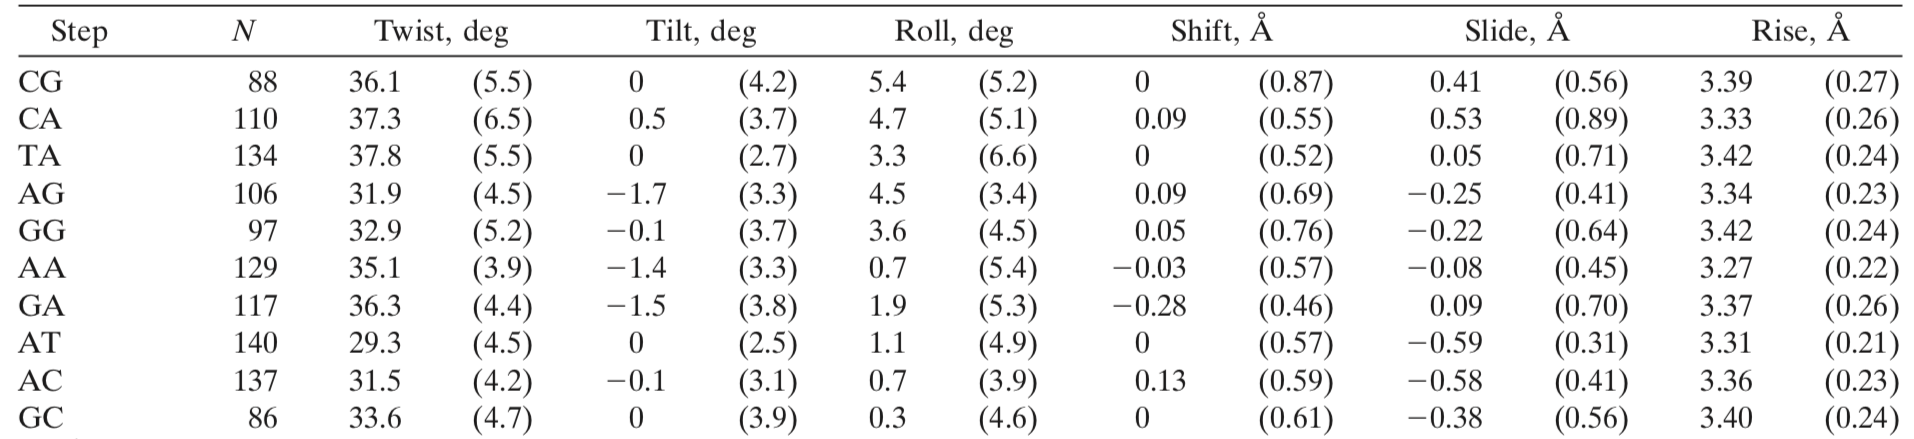
\includegraphics [width=\textwidth] {images/p1/olson_DNA_param}
  \caption{Матрица средних значений и отклонений динуклеотидных параметров из статьи \cite{olson_dna_1998}.} 
  \label{fig:p1:olson_DNA_param}
\end{figure}

Вычислив параметры отклонения ДНК в зависимости от типа динуклеотидного шага, а также дисперсии этих параметров, можно ставить задачу об оценке констант жесткости изгиба ДНК по этим различными параметрам $f_{ij}$ методом обратного гармонического анализа. В случае одномерной пружины, энергия которой описывается гармоническим законом $E=\frac{1}{2}fx^2$, распределение координаты согласно закону Больцмана будет выглядеть как $P(x) \sim \exp{-\frac{fx^2}{2kT}}$. Последнее является нормальным распределением с параметром дисперсии $\langle x^2 \rangle=kT/f$. Таким образом, мы установили связь дисперсии величины с константой жесткости.
В общем случае, когда энергия описывается функцией вида \ref{DNA_ener},  распределение состояний описывается многомерным нормальным распределением вида:
\begin{equation}
    P_{\mathbf X}(x_1,\ldots,x_k) = \frac{\exp\left(-\frac 1 2 ({\mathbf x}-{\boldsymbol\mu})^\mathrm{T}{\boldsymbol\Sigma}^{-1}({\mathbf x}-{\boldsymbol\mu})\right)}{\sqrt{(2\pi)^k|\boldsymbol\Sigma|}}
\end{equation}
где $|\boldsymbol\Sigma|=\det \boldsymbol\Sigma$, а $\boldsymbol\Sigma|$ - является матрицей ковариаций. Таким образом, несложно увидеть, что 
\begin{equation}
    \langle   \Delta\theta_{i} \Delta\theta_{j}\rangle=kT[{\boldsymbol F^{-1}}]_{ij}
\end{equation}
где ${\boldsymbol F}$ матрица коэффициентов $f_{ij}$, k - коэффициент Больцмана, $T$- конформационная температура, которую можно определить, например, сравнив получаемую гибкость с известными данными о персистентной длине. Константы жесткости доступны по адресу \url{https://web.archive.org/web/20151025043044/http://rutchem.rutgers.edu/~olson/pdna.html}.


Альтернативным подходом является вычисление характеристик динуклеотидных параметров путем молекулярного моделирования на основе атомистических силовых полей. Наиболее актуальной и современной здесь является работа \cite{walther_multi-modal_2020}. Авторы использовали наработки ABC консорциума, участники которого промоделировали методом атомистической молекулярной динамики все возможные последовательности тетрануклеотидов (всего их 136) \cite{dans_static_2019}. Из данных траекторий можно получить данные о флуктуациях различных параметров. Было показано, что распределения динуклеотидных параметров в некоторых случаях являются мультимодальными и их сложно аппроксимировать в виде одного многомерного гауссова распределения. Поэтому в данной статье некоторые распределения параметров описываются линейной комбинацией многомерных гауссовых распределений. Кроме того авторы делают попытку сделать коэффициенты $f_{ij}$ зависимыми от соседних с динуклеотидным шагом пар оснований - эффективно учитывая параметры изгибной жесткости ДНК на тетрануклеотидном уровне.

Суммируя вышесказанное, отметим достоинства и недостатки различных подходов. Гармоническое приближение при описании гибкости ДНК безусловно имеет свои ограничения, особенно в случаях, когда белок сильно деформирует ДНК. Например, в нуклеосомах динуклеотиды  пиримидин-пурин (YR) обычно выгибаются в сторону малой бороздки (параметр Roll отрицательный), в то же время из Рис. \ref{fig:p1:olson_DNA_param} видно, что в среднем в структурах динуклеотиды имеют положительный Roll, причем, динуклеотид TA (YR) больше склонен к положительному Roll, чем AT (RY). Однако предполагается, что при сильных изгибах (изломах, kinks) поверхность энергии устроена более сложным образом, и при комбинации с положительными значениями Slide - как раз AT выгоднее гнуться в сторону малой бороздки, чем TA \cite{wang_sequence-dependent_2010}. В этом плане мультимодальное приближение изгибной жесткости ДНК может являться более точным. Однако, для мультимодального приближения требуется большое количество качественных данных о динамике ДНК, которые, казалось бы, можно взять из молекулярно-динамических расчетов. Однако, здесь есть свой подводный камень - атомистические силовые поля, существующие на сегодняшний день, не совсем корректно описывают зависимость изгибной жесткости ДНК от последовательности в сравнении со структурными данными. Так, например, по данным вычислений молекулярной динамики максимальным значением параметра Roll Roll обладает динуклеотид TG \cite{pasi_muabc_2014}, а по данным анализа кристаллических структур CG.

\subsection{Программные продукты}
Для анализа геометрии ДНК был создан достаточно большое набор программных продуктов и методов, к ним можно отнести программы CompDNA\cite{gorin_b-dna_1995}, SCHNAaP \cite{lu_structure_1997}, Curves+ \cite{lavery_conformational_2009}, 3DNA \cite{lu_3dna_2008}. На данный момент наиболее используемой и поддерживаемой является программа 3DNA, которая позволяет не только анализировать структуру, но и реконструировать атомистическую структуру по набору параметров. Для анализа ширин и глубин бороздок ДНК может использовать программа Curves+.
Моделирование конформации ДНК в динуклеотидном приближении сводится к реализации либо алгоритмов минимизации конформации ДНК в пространстве параметров, либо к динамическим расчетам с помощью метода Монте-Карло. Многие такие программы разрабатывались для решения конкретных научных задач внутри научных групп, например, DNAminiCarlo (N.B. Ulyanov,
A.A. Gorin, V.B. Zhurkin), аналогичные подходы описаны в ряде статей \cite{norouzi_topological_2015,kulaeva_internucleosomal_2012}, недавно появилась программа MC-enNN и веб-сервер к ней \cite{walther_multi-modal_2020}. В нашей научной группе проводится разработка программы с открытым программным кодом PyNAMod
 \url{http://github.com/intbio/PyNAMod}, способной моделировать ДНК, включая ДНК-белковые комплексы в динуклеотидном приближении методами минимизации геометрии ДНК, а также методом цепей Монте-Карло.

\subsection{Алгоритмы интегративного моделирования}
\label{sec:p1:int_algo}
Введение дополнительных ограничений при моделировании ДНК в динуклеотидном приближении, а также учет стерических ограничений путем конвертации структуры из пространства динуклеотидных параметров в атомистическую структуру, позволяют сформулировать подходы для интегративного моделирования ДНК и комплексов-ДНК белок на основе различных экспериментальных данных.

В реализованных нами подходах при минимизации конформации ДНК в динуклеотидном приближении в энергию системы вводились дополнительные члены, соответствующее отклонению набора расстояний от целевых значений, измеренных при помощи экспериментальных методов, например, spFRET. Алгоритм действия программы изображен на Рис. \ref{fig:p1:int_mod_dinuc}. На вход программа получает начальные структуры в формате PDB. Измерения методом spFRET дают информацию о расстояниях между парами меток. Алгоритм последовательно оптимизирует координаты нуклеотидных пар таким образом, чтобы привести их геометрию в соответствие с результатами spFRET. В ходе работы алгоритма учитываются ограничения, связанные с жесткостью ДНК.


\begin{figure}[H] 
  \center
  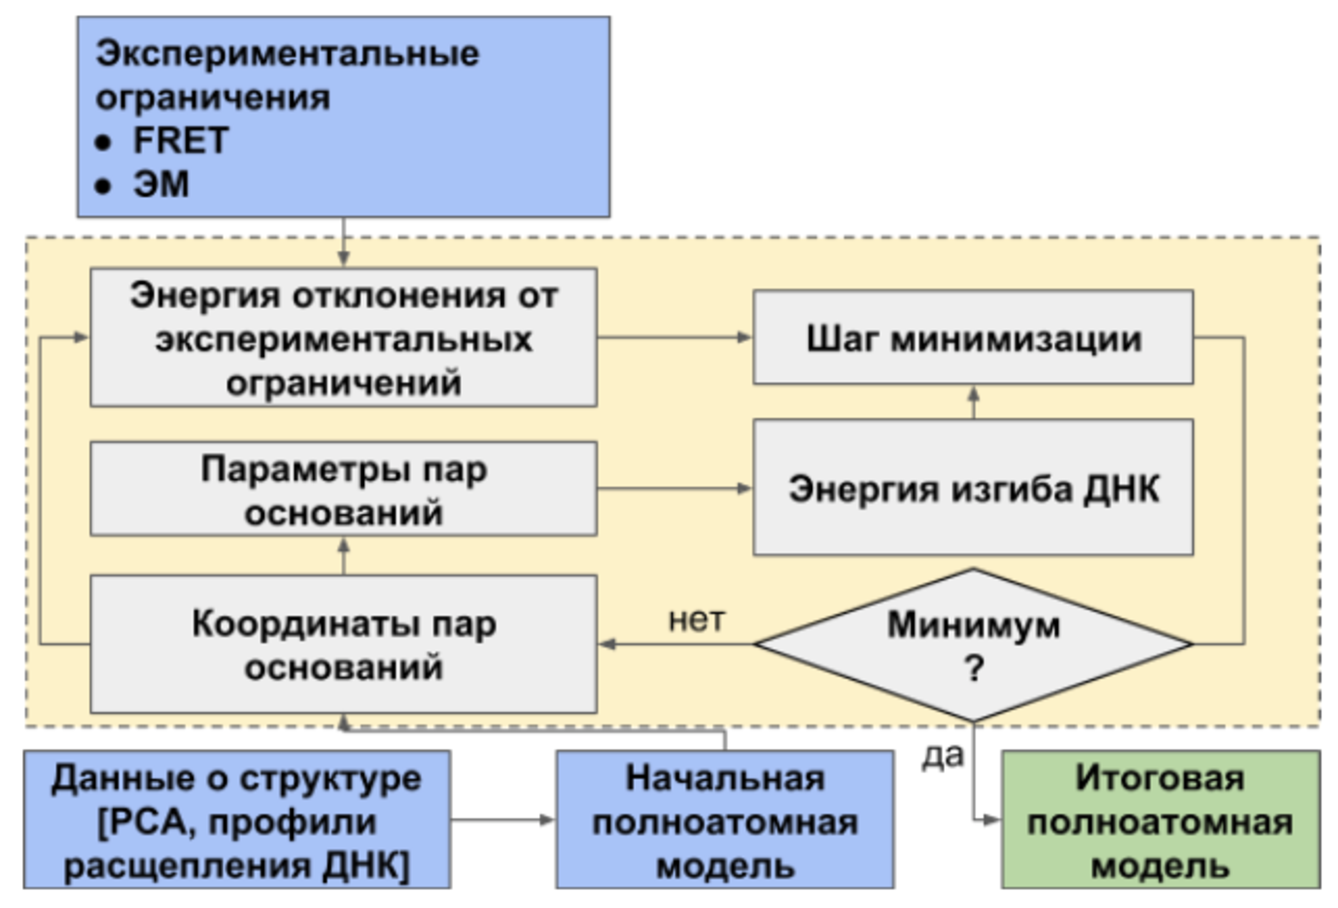
\includegraphics [width=\textwidth] {images/p1/int_mod_dinuc}
  \caption{Алгоритм интегративного моделирования на основе моделей ДНК в динуклеотидном приближении.} 
  \label{fig:p1:int_mod_dinuc}
\end{figure}
%\section{Методы моделирования супрануклеосомной структуры хроматина}
\section{Методы моделирования супрануклеосомной структуры хроматина}
% сделать на основе https://docs.google.com/document/d/1A_RRCcKiU5YPzdSMHhqiwX-g2PkqbeQ4iB5KrB0_MFI/edit?usp=sharing

    В последние годы благодаря совершенствованию экспериментальных технологий наметилась долгожданная конвергенция методов структурной биологии и методов геномики в изучении организации хроматина на молекулярном уровне. Благодаря успехам крио-электронной микроскопии, мы получаем все больше информации о структуре не только нуклеосом, но и супрануклеосомных структур, а благодаря развитию методов геномики и 3-D геномики все более высокого разрешения, стало возможным определять контакты между локусами ДНК с суб-нуклеосомным разрешением (в частности, методы Micro-C, Micro-C-XL и др.) и определять положение и состав нуклеосом вдоль генома (напр. методы MNase-seq, MNase-ChIP-seq). Возникает необходимость в интерпретации экспериментальных данных и построении физических молекулярных моделей укладки хроматина на супрануклеосомном уровне с учетом реальных геометрических и топологических параметров молекул белков и ДНК, а также динамического характера этих взаимодействий.

    Так как изучение организации хроматина на супрануклеосомном уровне довольно давно представляет собой фундаментальную задачу для молекулярной и клеточной биологии (примем за дату начала год открытия нуклеосомы и структуры в виде ``бусин на нити'' - 1974 \cite{kornberg_chromatin_1974}), было разработано множество подходов к молекулярному моделированию укладки нуклеофиламента. Большую часть прошедшего времени сомнений в концепции 30-нанометровой фибриллы не возникало (идею 30-нанометровой фибриллы предложили в 1980 году, серьезные аргументы против появились в 2000-ых, 2010-ых  см., например, \cite{joti_chromosomes_2012,razin_chromatin_2014}). Поэтому подавляющее число работ по молекулярному моделированию хроматина на супрануклеосомном уровне являются по сути работами по моделированию 30-нанометровой фибриллы, что, не умаляя их методологической значимости, значительно снижает ценность результатов и приводит к необходимости проведения работ по молекулярному моделированию хроматина на супрануклеосомном уровне с учетом современных знаний о нем.  При этом изучение предыдущей литературы по данной теме все-таки необходимо, так как ее авторы достигли значительных результатов в разработке математического и концептуального  аппарата для моделирования хроматина на этом уровне вообще. Например, в работе 2015 года Norouzi, D. \& Zhurkin, V. B. Topological Polymorphism of the Two-Start Chromatin Fiber \cite{norouzi_topological_2015} авторы с помощью своей модели изучили все возможности организации двухстартовой хроматиновой фибриллы (есть два гипотетических типа организации 30-нанометровой хроматиновой фибриллы: соленоидная - одностартовая фибрилла - и зигзагом - двухстартовая фибрилла - причем тип фибриллы коррелирует с длиной ликерного участка), т.е. смоделировали все возможные ее конформационные варианты. Фибриллы моделировали симметричными и регулярными, а для расчетов вводилось 4 параметра суперспирализации: кручение, подъем, наклон нуклеосом и диаметр. Энергия фибриллы задавалась как сумма четырех слагаемых: эластической энергии линкерной ДНК, стерического отталкивания, электростатики (рассчитываемой с помощью кулоновского потенциала), феноменологического взаимодействия между двумя ``сложенными в стопку'' нуклеосомами. При оптимизации энергии фибриллы с учетом параметров суперспирализации исследователи впервые обнаружили два типа топологического перехода в ней: путем резкого на 360 градусов поворота в кручении линкера и путем скрещивания линкеров. Даже при моделировании структуры, отличной от 30-нанометровой фибриллы, эти принципы могут быть релевантными, так как позволяют рассчитать такие общие вещи, как энергию комплекса ДНК-нуклеосома, его оптимальную геометрию в зависимости от длины линкеров и внешних факторов. Эти же авторы  в более поздней  работе того же года продолжали исследовать топологический полиморфизм хроматиновой фибриллы, пытаясь установить связь между длиной линкеров и спецификой сверхспирализации ДНК (связанной с уровнем транскрипции). Интересно, что для нахождения оптимальной конформации линкерной ДНК использовался мезоскопический подход: ДНК моделируется динуклеотидными ``шагами'', его траектория описывается с помощью шести параметров: Tilt, Roll, Twist, Shift, Slide, Rise. Мезоскопический подход был  предложен в статье Olson et al., 1993 \cite{olson_influence_1993}, данные шестимерные координаты - в работе Dickerson et al., 1989 \cite{dickerson_definitions_1989}. Оба этих концептуальных инструмента широко используются в моделировании хроматина на низких уровнях компактизации (10-нанометровой фибриллы и следующем) и никак не зависят от концепции 30-нанометровой фибриллы, что делает их полезными и для моделирования альтернативных этой фибрилле структур. Крайне эффективным для молекулярного моделирования супрануклеосомного уровня компактизации хроматина являются методы, основанные на принципах Монте-Карло. Познакомиться с ними можно, например, в работе — Norouzi, D. \& Zhurkin, V. B. Dynamics of Chromatin Fibers: Comparison of Monte Carlo Simulations with Force Spectroscopy \cite{norouzi_dynamics_2018}. Шаги симуляции следующие: случайный выбор одной пары оснований в подвижном линкере и изменение его шести параметров, обновление позиций нуклеосом в нуклеосомном массиве, вычисление разницы в энергии между старым и новым состоянием и выполнение теста Метрополиса. Варьируя величину внешних сил, степень развернутости (unwrapping) нуклеосом, длину нуклеосомных повторов (NRL - nucleosome repeat length) - среднее расстояние между центрами соседних нуклеосом и значение энергии стэкинга (stacking energy), исследователи провели серию симуляций, каждая из которых включала около 100 миллионов описанных выше шагов. Подобный подход, особенно его вариант - моделирование путем имитации отжига - позволяет довольно эффективно находить глобальный энергетический минимум в заданной системе.
    
    Также часто применяется для решения задач моделирования хроматина на разных уровнях организации метод огрубленного моделирования (coarse-grained). Суть метода состоит в представлении молекул и молекулярных структур (например, нуклеосом) простыми телами и поверхностями: сферами, цилиндрами, плоскостями. Такое приближение значительно упрощает вычисления и позволяет проводить однозначный анализ за приемлемое время. Однако при этом исходные данные подвергаются соответствующей деформации - результат моделирования соответствует им не полностью, он также зависит от выбранной стратегии огрубления. Хроматиновые фибриллы и их динамику обычно моделируют как цепочки из шаров или как червеобразные структуры \cite{korolev_systematic_2018,savelyev_molecular_2009,ozer_chromatin_2015}. Несмотря на популярность метода огрубленного моделирования в области изучения структуры хроматина, он является далеко не оптимальным для решения этих задач: исходные данные не используются полностью, искажаются, что может быть критичным, когда речь заходит об изучении укладки 10-нанометровой фибриллы, так как образуемая ею структура зависит от не учитываемых в огрубленных методах параметров - например, длины линкера \cite{norouzi_topological_2015,nikitina_dna_2017,norouzi_topological_2015}. Для адекватного моделирования структуры хроматина требуется основывать его на данных высокого разрешения (например, современных протоколов Hi-C), причем они не должны искажаться так сильно, как в методе огрубленного моделирования. Таким образом необходимо разработать новый, более чувствительный к данным и параметрам наподобие длины линкеров подход. 

    Важно отметить, что большинство описываемых выше подходов основаны на ``закрытом'' программном обеспечении. Авторы либо не предоставляют доступа к программному обеспечению, либо оно является слабо используемым, поскольку к нему нет описания, либо возникают проблемы с переносимостью.

\begin{figure} [h!]
    \centering
    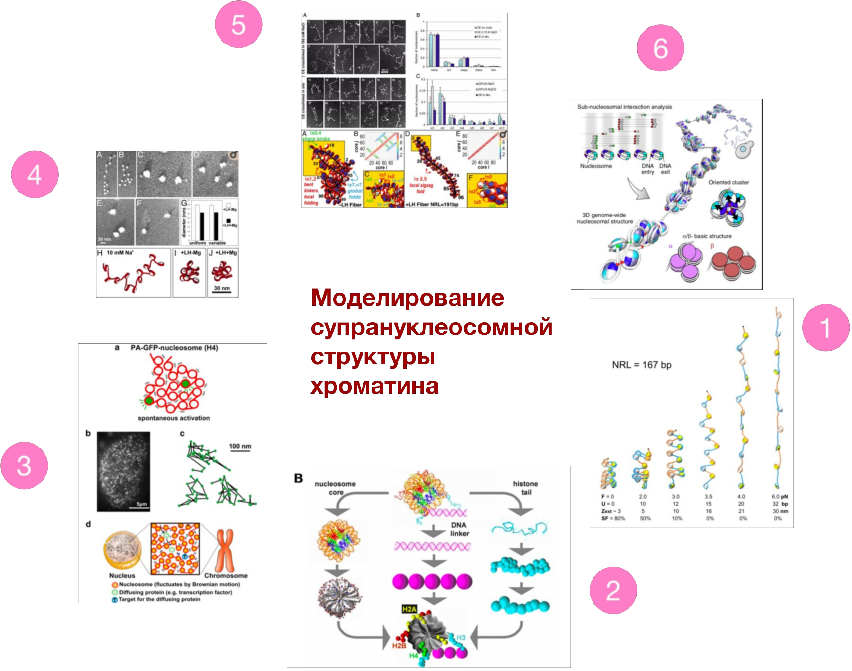
\includegraphics [width=\textwidth]{images/p1/part1_4_cm/part1_4_cm_f6.pdf}
    \caption[Подходы к моделированию супрануклеосомной структуры]{Подходы к моделированию супрануклеосомной структуры, в том числе с учетом экспериментальных данных. (1) - Молекулярная динамика с использованием принципов Монте-Карло \cite{norouzi_dynamics_2018}; (2) - Огрубленное моделирование \cite{schlick_monte_2009}; (3) - (6) : интегративные методы. (3) - Моделирование на основе данных метода Single nucleosome imaging  - отображения одиночных нуклеосом \cite{maeshima_chromatin_2014}; (4), (5) - Моделирование на основе данных метода EMANIC - метода обнаружения нуклеосом с помощью электронной микроскопии \cite{grigoryev_evidence_2009}, \cite{grigoryev_hierarchical_2016}); (6) - Моделирование супрануклеосомной структуры на основе данных модифицированного Micro-C   \cite{ohno_sub-nucleosomal_2019}}.
    \label{fig:p1_4:f6}
\end{figure}


    Важным подходом является интеграции различных экспериментальных данных при построении моделей - данный подход называется интегративным моделированием. В применении к супрануклеосомной структуре он на наш взгляд развит весьма слабо. На данный момент по данным литературы известна лишь одна попытка интеграции данных Micro-C с методами моделирования. Работа опубликована в 2019 году \cite{ohno_sub-nucleosomal_2019}. В ней приведены довольно убедительные доказательства существования определенных супрануклеосомных структур в геноме пекарских дрожжей, альтернативных отвергнутой  хроматиновой фибрилле, - хроматиновых альфа-тетраэдров и бета-ромбов - то есть этой работой был сделан большой шаг на пути к определению структуры хроматина на до сих пор не исследованных уровнях компактизации генома. Молекулярное моделирование проводилось на основании теоретической модели нуклеосомы - как комплекса из гистонового октамера и ассоциированной с ним ДНК — и данных Micro-C, позволяющих различать точки ``входа'' и ``выхода'' ДНК в/из нуклеосом. Такой комбинированный метод был назван Hi-Co. Само моделирование проводилось с помощью подхода имитации отжига в методе молекулярной динамики. Имитация отжига была необходима для оптимизации позиций и ориентаций отдельных нуклеосом, остальные структурные факторы, такие как, например,  линкерная ДНК (ее длина), были неявно включены в потенциалы и по сути не рассматривались детально. Несмотря на важное значение, подходы моделирования в работе Ohno et al.  не вполне реалистичны, так как, например,  отсутствуют в явном виде линкерная ДНК, а следовательно не учитывается влияние топологии и кручения ДНК важные для понимания многих функциональных процессов и состояний в хроматине. Также в подходе авторов не предполагался учет нуклеосом различного типа и возможного откручивания ДНК от нуклеосомы с изменением углов входа/выхода ДНК. Кроме того работа Ohno et al. была посвящена изучению генома дрожжей — это значит, что непосредственной значимостью для медицины она не обладает. Требуется провести аналогичное исследование генома высших, многоклеточных эукариот и человека.

%картинка
\begin{figure} [h!]
    \centering
    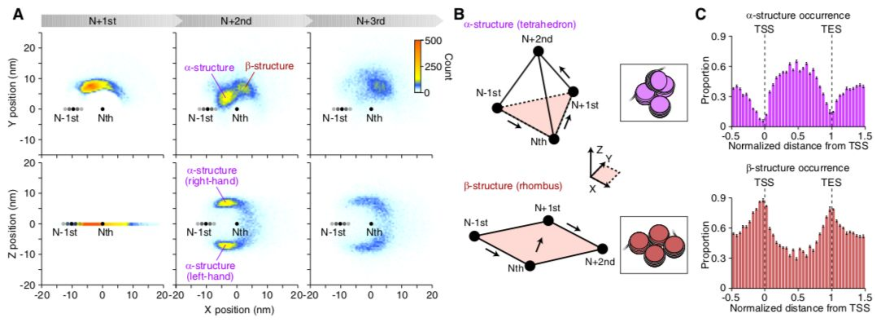
\includegraphics[width=\textwidth]{images/p1/part1_4_cm/part1_4_cm_f7.pdf}
    \caption[Визуализация анализа данные Micro-C, Ohno et al., 2019]{Визуализация результатов анализа взаимного расположения нуклеосом в пространстве и выявленные в результате него мотивы супрануклеосомной структуры ДНК из статьи Ohno et. al, 2019}
    \label{fig:p1_4:f7}
\end{figure}

Для моделирования супрануклеосомной укладки фибрилл алгоритмы, предложенные нами в пункте \ref{sec:p1:int_algo}, могут быть адаптированы путем включения дополнительных данных из экспериментов Micro-C, а также данных о позициях нуклеосом из экспериментов MNase-seq, ATAC-seq (см. Рис. \ref{fig:p1_4:f8}). 
     Расчет обобщенных переменных из атомистической структуры и восстановление координат из набора переменных, описывающих геометрию ДНК в динуклеотидном приближении, производится при помощи программы 3DNA \cite{lu_3dna_2003}, либо при помощи разрабатываемой программной библиотеки PyNAMod.      Учет положения и геометрии белковых компонент можно производить в том же приближении: для этого необходимо определять их ориентацию относительно ключевых динуклеотидов. Например, при определении гистонового ядра нуклеосомы, отсчитывать его положение относительно диадного динуклеотида.
    Дополнительно в физическую модель нуклеосомной фибриллы вводятся парные потенциалы для учета исключенного объема и электростатических взаимодействий между соседними нуклеосомами, что необходимо для учета изменяющих заряд посттрансляционных модификаций гистоновых хвостов.
     При моделировании цепочек нуклеосом, вводятся ограничения на расстояния, описывающие межнуклеосомные контакты. Возможно также введение дополнительного потенциала, позволяющего нуклеосомам смещаться относительно их изначальных положений (что обосновано точностью определения их положения в эксперименте).   В рамках описываемой физической модели нуклеосомной фибриллы можно создавать модели организации хроматина путем применения численных методов минимизации значений функции, например метода градиентного спуска, однако, для обнаружения глобального минимума, а также создания множественной выборки из конфигурационного пространства более применимы стохастические подходы, такие как метод  Монте-Карло с алгоритмом Метрополиса.

\begin{figure} [h!]
    \centering
    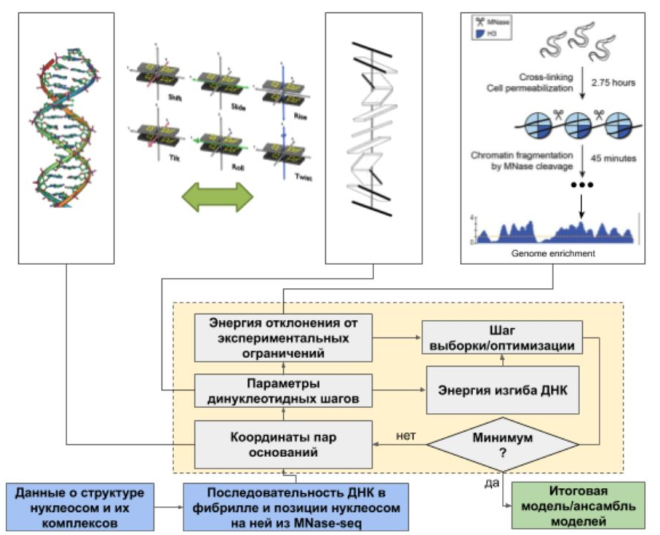
\includegraphics [width=\textwidth]{images/p1/part1_4_cm/part1_4_cm_f8.pdf}
    \caption[Алгоритмы интегративного моделирования нуклеосомных фибрилл]{Алгоритмы интегративного моделирования нуклеосомных фибрилл. Слева вверху - схематическое описание ДНК в приближении динуклеотидных шагов. Справа вверху - сокращенное схематическое представление методов Micro-C/MNase-seq/MNase-ChIP-seq. Снизу - Описание подхода интеграции экспериментальных данных в физическую модель нуклеосомных фибрилл.}
    \label{fig:p1_4:f8}
\end{figure}











\section{Основы некоторых экспериментальных методов}
%\subsection{Футпринтинг ДНК с использованием гидроксил-радикалов}
\subsection{Методы футпринтинга ДНК}
Одним из подходов к изучению структуры ДНК и ДНК-белковых комплексов являются методы физического, химического или ферментативного футпринтинга (от англ. footprint - след). Идея методов состоит в обработке ДНК определенными агентами, которые вносят изменения в ее химическую структуру в зависимости от ее конформации, состава или взаимодействия с другими макромолекулами, с последующим анализом продуктов реакции для установления мест химических реакций вдоль ДНК.

К физическим методам относят облучение ДНК ультрафиолетом \cite{becker_ultraviolet_1988} или рентгеном, что приводит к разрыву ДНК в областях не защищенных белком. С помощью секвенирующего гель электрофореза можно определить длины продуктов реакций и следовательно участки взаимодействия с белком. Аналогичный подход может быть осуществлен с использованием генерируемых в реакционной смеси гидроксил радикалов химическими методами. Методам гидроксильного футпринтинга посвящена глава \ref{part5_hrf} данной диссертационной работы. Наиболее популярным методом ферментативного футпринтинга является использование фермента ДНКазы I, обладающего выраженной эндонуклеазной активностью. К плюсам такого подхода относится простота осуществления эксперимента, к минусам большой размер фермента (около 4 нм), что уменьшает детальность футпринтинга, и наличие некоторой специфичности по последовательности (гидролизует ДНК преимущественно около пиримидинов). Еще одним интересным методом химического футпринтинга является футпринтинг с использованием перманганата калия. Перманганат калия связывается с тиминами в одноцепочечной ДНК, окисляет их, что приводит в конченом итоге к разрыву в ДНК. Таким образом можно исследовать локализацию пузырей транскрипции в геноме, нестандартных ДНК структур  \cite{kouzine_permanganates1_2017}. Футпринтинг с использованием диметилсульфата (ДМС) используется также для изучения ДНК-белковых взаимодействий. ДМС индуцирует метилирование остатков гуанина. Два образца обрабатывают пиперидином, чтобы вызвать химическое расщепление остатков гуанина, модифицированного ДМС, с последующим расщеплением рестрикционными ферментами. После маркировки образцы запускают параллельно на геле для визуализации. Отсутствующие полосы в образце, связанном с белком, соответствуют остаткам гуанина, защищенным от модификации посредством взаимодействия \cite{hornstra_vivo_1993}.

%\subsection{ФРЕТ спектроскопия и микроскопия}
\subsection{FRET спектроскопия и микроскопия}
%\todo{2S Из файла Armeev\_disser.pdf - со стр. 23 весь п. 1.4 с картинками. НО - нужно весь текст переписать так, чтобы его не детектировал антиплагиат - нужно чтобы подряд не было 3 похожих слов (!) можно перефоразировать, заменять на синонимы, менять местами слова}
%то есть до страницы 36 включительно?


\subsubsection{Ферстеровский резонансный перенос энергии}

    Ферстеровский резонансный перенос энергии (Forster resonance energy transfer, FRET) это эффект безызлучательного переноса энергии с одного красителя-флуорофора на другой. Пару (или более) флуорофоров подбирают таким образом, чтобы спектр поглощения акцептора перекрывался со спектром флуоресценции донора. Флуорофоры могут быть пришиты к аминокислотам или азотистым основаниям ДНК с помощью различных линкерных молекул. По определение эффективность FRET - это отношение вероятности переноса энергии с донора на акцептор по отношению ко всем другим переходам в расчете на событие возбуждение донора:
\begin{equation}
    E_{FRET} = \frac{k_\text{ET}}{k_f + k_\text{ET} + \sum{k_i}}
\end{equation}    
 где $k_{ET}$ - скорость переноса энергии с донора на акцептор, $k_f$ - скорость процесса флуоресценции донора,  $k_i$ - скорости других неизлучательных процессов релаксации донора, за исключением переноса энергии на акцептор.
    Эффективность переноса энергии существенно зависит от расстояния между метками и может быть описана следующей формулой:

\begin{equation}
    E_{FRET}=\frac{1}{1+(R/R_0)^6}
    \label{fret_E}
\end{equation}
    где R - расстояние между метками, $R_0$ - радиус
     Ферстера, расстояние между метками, отвечающее 50\% эффективности переноса энергии между флуорофорами (см. Рис. \ref{fig:p1_5_fret:f3}). Согласно данной формуле, измеряя эффективность FRET возможно вычислить расстояние между участками меченой макромолекулы. Для каждой пары меток радиус Ферстера индивидуален, он зависит от ряда факторов, в том числе от квантового выхода флуоресценции донора, ориентации красителя на поверхности молекулы (ориентационный фактор), коэффициента преломления среды и т.д. 

\begin{figure} [h!]
    \centering
    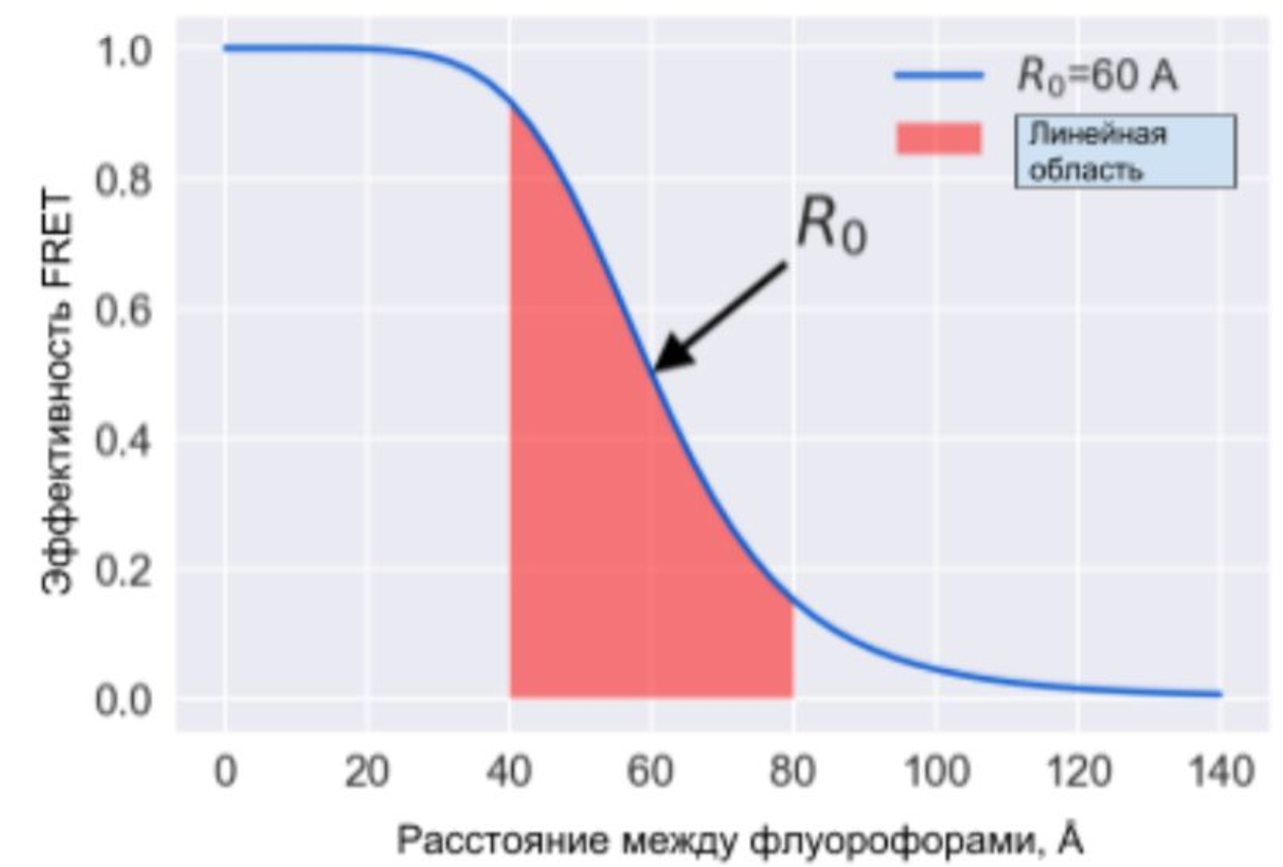
\includegraphics[width=\textwidth]{images/p1/part1_5_fret/part1_5_fret_f3.pdf}
    \caption[Зависимость эффективности переноса энергии от расстояния между флуорофорами.]{Зависимость эффективности переноса энергии от расстояния. Стрелкой показана величина Ферстеровского радиуса. Красным показана область изменений, близкая к линейной. }
    \label{fig:p1_5_fret:f3}
\end{figure}

    Эффективность переноса энергии может быть выражена через отношение времен жизни флуоресценции донора в отсутствии и присутствии акцептора:
\begin{equation}
    E_{FRET}= 1-\tau_{D}^{'}/\tau_D
\end{equation}
    где $\tau_{D}^{'}$ - время жизни флуоресценции донора в присутствии акцептора,  $\tau_D$ время жизни донора в отсутствии акцептора.
    
    Альтернативным является выражение эффективности переноса через величины интенсивности флуоресценции донора и акцептора:
    
\begin{equation}
   E_{FRET}=\frac{F_A}{F_A+\gamma F_D}
   \label{eq:p1:fret}
\end{equation}
    где $F_A= I_A - B_A - \alpha_{DA} (I_D - B_D) - D_{ex}$, $F_D = I_D - B_D - \alpha_{AD} (I_A - B_A )$ и 
В последних формулах $I_A$ и $I_D$  - регистрируемые интенсивности сигнала акцептора и донора, соответственно; $B_A$ и $ B_D$ - уровни фонового сигнала в канале акцептора и донора, соответственно;  $\alpha_{DA}$ и $\alpha_{AD}$ - перекрестные коэффициенты (crosstalk coefficients), характеризующие долю флуоресценции донора, регистрируемую в канале акцептора ( $\alpha_{DA}$ ), и долю излучения акцептора, регистрируемую в канале донора ( $\alpha_{AD}$ ). Поправочные коэффициенты помогают учитывать особенности  оптической схемы конфокального микроскопа или спектрофлуориметра, для разных пар флуоресцентных меток они отличаются. $D_{ex}$ - это величина сигнала прямого возбуждения акцептора (возникающая в следствие возможного поглощения фотонов акцептором на длине волны поглощения донора). $\gamma$ - так называемый фактор детекции, он позволяет учитывать различия в эффективностях детекции флуоресценции $(\eta)$ донора и акцептора и различия в их квантовых выходах флуоресценции ($\Phi$) \cite{dahan_ratiometric_1999}. Фактор детекции может быть представлен в виде:

\begin{equation}
    \gamma = \gamma_{instrument} \gamma_{dye} = \frac{\eta_A \Phi_A}{\eta_D \Phi_D}
\end{equation}
где $\Phi$ - квантовый выход, $\eta$ - эффективность детекции.
    Эффективность детекции флуоресценции зависит от спектральной чувствительности детекторов (лавинных фотодиодов или фотоэлектронных умножителей) и спектральных характеристик оптических элементов, через которые проходит сигнал от образца. 
    Измерение фактора детекции в ряде случаев может быть затруднено и его принимают за единицу. В таком случае измеряемая по формуле (\ref{eq:p1:fret}) величина является не истинным коэффициентом переноса, такую величину называют ``коэффициентом близости'' (PR - proximity ratio). Коэффициент близости нельзя непосредственно связать с расстоянием между флуоресцентными метками, однако, используя этот коэффициент можно делать выводы о гетерогенности образца, и о качественных эффектах сближения или удаления частиц.

\subsubsection{Детекция сигнала от одиночных молекул}
    Эффективность FRET может быть измерена в объеме сразу от многих частиц при помощи прибора спектрофлуориметра. В этом случае измеренный сигнал соответствует некоторому среднему сигналу от ансамбля молекул \cite{klose_simulation_2012}. Такой усредненный сигнал может не соответствовать ни одному конкретному состоянию системы на молекулярном уровне, а являться суперпозицией нескольких состояний разных частиц. Чтобы добиться связи сигнала FRET с конкретными состояниями молекулярной системы, необходимо, как минимум, измерять эффективности FRET у одиночных частиц, такой метод называется spFRET (single particle FRET). С помощью метода spFRET возможно оценивать как средние расстояния \cite{okumus_vesicle_2004}, так и временную динамику изменения расстояний между метками \cite{li_rapid_2005}. Вопрос заключается в том, каким образом снимать сигнал от одной частицы. Одни вариант заключается в иммобилизации частиц на поверхности. Иммобилизовав частицы, можно использовать подходы, основанные на эффекте полного внутреннего отражения, которые позволяют проводить измерения в тонком слое частиц у поверхности \cite{roy_practical_2008}. Преимущество такого метода в возможности наблюдения эволюции сигнала сразу для многих частиц в поле зрения микроскопа. Недостатком является возможные взаимодействия частиц с подложкой, которые могут повлиять на их структуру и динамику \cite{zanetti-domingues_hydrophobic_2013}. Альтернативных подход основан на измерении флуоресценции от единичных молекул, свободно диффундирующих сквозь фокальный объем конфокального флуоресцентного микроскопа (см. Рис. \ref{fig:p1_5_fret:f4}). Для реализации этого метода необходимо, чтобы исследуемые частицы находились в достаточно низкой концентрации, чтобы одновременно в фокальном объеме находилось не более одной частицы. Метод требует наличия конфокального микроскопа, чувствительных лавинных фотодиодов (APD или SAPD). По мере проплывания частиц можно собирать необходимую статистику, однако поскольку проплывание обычно занимает миллисекунды, присутствуют ограничения на возможности слежения за динамикой процессов внутри частицы. 

\begin{figure} [h!]
    \centering
    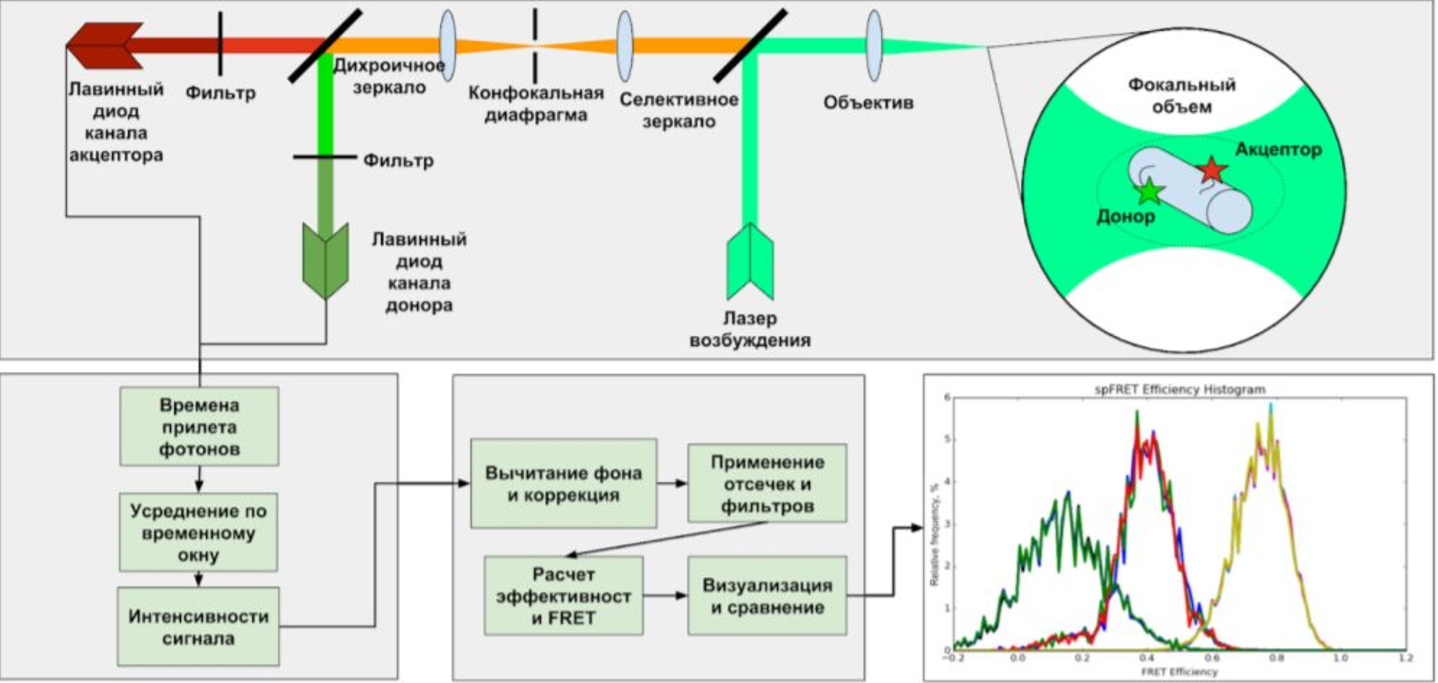
\includegraphics[width=\textwidth]{images/p1/part1_5_fret/part1_5_fret_f4.pdf}
    \caption[Схема экспериментов spFRET]{Схема экспериментов spFRET. Один лазер возбуждает флуоресценцию. Флуоресценция из конфокального объема собирается на лавинных фотодиодах. Времена прилета фотонов анализируются программным обеспечением микроскопа, либо специализированным ПО.}
    \label{fig:p1_5_fret:f4}
\end{figure}


\subsubsection{Подходы к измерению эффективности FRET}
Величина $E_{FRET}$, как следует из вышеприведенных формул, может быть рассчитана двумя способами, либо через время флуоресценции донора \cite{sisamakis_accurate_2010}, либо через измерение интенсивностей свечения донора и акцептора. Последний подход называется ратиометрическим подходом. 

Для того, чтобы измерить времена флуоресценции необходимо существенно более сложное оборудование. Порядок времен флуоресценции составляет порядка наносекунд, поэтому требуются лазерные источники и синхронизированные детекторы, способные работать в пикосекундном диапазоне. Такой подход реализован в методе TCSPC (Time Correlated Single Photon Counting). Он же используется в популярном методе микроскопии супер разрешения FLIM (fluorescence-lifetime imaging microscopy).
Важным преимуществом данного метода является отсутствие необходимости учитывать эффекты, связанные с мощностью осветителя, различными параметрами оптической системы и системы детекции, влияющими на корректировочные факторы. Наличие временного разрешения пикосекундрного диапазона, также позволяет эффективно проводить отсеивание шумовых всплесков в сигнале.

Ратиометрический подход может быть реализован с использованием более простого оборудования, например, конфокального микроскопа с лазером непрерывного излучения. Однако, этот подход чувствителен к шумовым эффектам, связанным с рассеянием света, колебаниям интенсивности лазера. Для соотнесения измеренных интенсивностей с реальными фотофизическими процессами необходимо предварительно измерить фактор детекции $\gamma$. Отдельной проблемой является то, что данный фактор может зависеть от конформационных изменений в молекулярной системе, так как квантовые выходы чувствительны к окружению флуорофоров.


\subsubsection{Подходы к измерению интенсивности флуоресценции spFRET от одиночных молекул}

Интенсивности флуоресценции в радиометрическом подходе, в зависимости от приборных возможностей, регистрируют либо в виде временного ряда, описывающего прилет отдельных фотонов (single photon counting), либо в виде некоторого сигнала, описывающего зависимость интенсивности от времени. В последнем случае прибор будет проводить усреднение (бинирование) сигнала с некоторым временным интервалом. В случае измерения spFRET в растворе, данный временной интервал необходимо выбирать с учетом кинетики проплывания частиц через фокальных объем микроскопа.
Для оценки времени проплывания частицы через фокальный объем можно использовать диффузионное соотношение:
 
\begin{equation}
    \tau \approx \langle x^2 \rangle / 2D
\end{equation}
    где $\tau$ - время проплывания, $D$ - коэффициент диффузии, $x$ - координата частицы вдоль одной из осей системы координат.
    
Для обработки непосредственно времен прилета фотонов также разработаны различные алгоритмы, позволяющие выделять внутри временного ряда события, связанные с проплыванием частиц и оценивать фоновых сигнал \cite{ingargiola_fretbursts_2016}. 
Оценку фонового сигнала можно проводить непосредственно анализируя правый край гистограммы распределения временных задержек между прилетом фотонов. Поскольку вероятность прилета фотонов за некоторый интервал времени описывается распределением Пуассона
\begin{equation}
    P[N(t)=k](t) = \frac{e^{-\lambda t} (\lambda t)^k}{k!}
\end{equation}
можно показать, что задержки распределены согласно экспоненциальному распределению:

\begin{equation}
    P(t)= \lambda e^{- \lambda t}
\end{equation}
где $\lambda$ - средняя частота детекции фотонов.
На практике распределение будет состоять из суммы распределения фонового сигнала и сигнала от проплывающих частиц.


% \begin{figure} [h!]
%     \centering
%     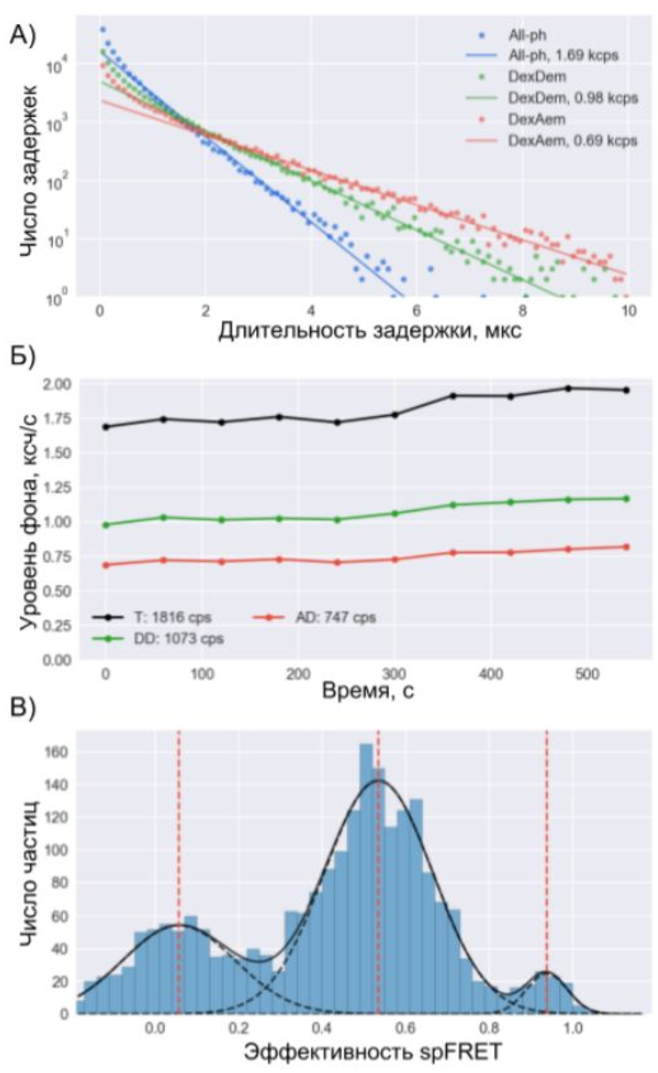
\includegraphics[width=100pt]{images/p1/part1_5_fret/part1_5_fret_f5.pdf}
%     \caption{А) гистограмма длительностей задержек между соседними фотонами в канале донора (зеленый), акцептора (красный), в обоих каналах (синий). Б) изменение уровня фона в ходе эксперимента. В) Типовая гистограмма эффективности spFRET со вписанными в нее тремя функциями Гаусса}
%     \label{fig:p1_5_fret:f5}
% \end{figure}

\subsubsection{Измерение фактора детекции}
При ратиометрическом измерении FRET вычисление истинного $E_{FRET}$ требует определения корректирующего фактора $\gamma$. Данный фактор позволяет перемасштабировать отношение регистрируемых интенсивностей сигнала в каналах донора и акцептора, чтобы учесть разницу в квантовых выходах красок и эффективности детекции фотонов от разных красок прибором. Также фактор детекции может изменяться целенаправленно варьируя параметры прибора для достижения большего разрешения в областях расстояния между метками большими или меньшими радиуса Ферстера \cite{gansen_structural_2009}. 

Для измерения параметра $\gamma$ можно использовать ряд экспериментальных методик. Квантовые выходы измеряют их сравнения с квантовыми выходами известных красителей \cite{williams_relative_1983}. Инструментальную часть фактора, $\gamma_{instrument}$, можно вычислить используя формулу:
\begin{equation}
    \gamma_{instrument} = \frac{m_{A}^{smF} m_{D}^{Abs} \Phi_{D}}{m_{D}^{smF} m_{A}^{Abs} \Phi_{A}}
\end{equation}
    где $m_{A}^{smF}$ и $m_{D}^{smF}$ - производные интенсивности флуоресценции акцептора и донора по концентрации для заданного лазера, $m_{A}^{Abs}$ и $m_{D}^{Abs}$ - производные поглощения акцептора и донора от концентрации, измеренные на длинне волны возбуждения донора, $\Phi_A$ и $\Phi_D$ квантовые выходы акцептора и донора. Более подробно методика описана в работе \cite{ferreon_interplay_2009}.

Альтернативой измерению фактора детекции в отдельных экспериментах (в том числе с применением спектрофотометра), является его измерение непосредственно во время эксперимента. Например, метод ALEX FRET (alternating laser excitation FRET) использует чередующиеся вспышки двух лазеров, возбуждающих поочередно донор или акцептор. Такой метод позволяет сразу определить стехиометрию красок в проплывающем комплексе. Измеряя эффективность переноса для комплексов с различной стехиометрией можно рассчитать фактор детекции \cite{lee_accurate_2005}. 

% \subsection{Детекция структурной гетерогенности в образце}
%     Чаще всего, результаты измерения эффективности spFRET анализируют путем построения частотных гистограмм (Рис. 5 В). Полученные распределения затем аппроксимируют Гауссовыми функциями, положение которых принимают за среднюю эффективность переноса энергии для субпопуляции частиц. Средняя эффективность переноса энергии затем может быть использована для оценки среднего расстояния между флуоресцентными метками. Помимо средней эффективности, информацию об исследуемой системе можно получить из формы и ширины распределения эффективностей spFRET [60,61]. Уширение распределений может свидетельствовать как о статической структурной гетерогенности образца, так и о динамической структурной гетерогенности образца: под статической гетерогенностью понимают наличие в образце смеси частиц с разными расстояниями между метками, изменение расстояний при этом либо не происходит, либо происходит на временах, значительно превышающих времена диффузии частиц сквозь фокальный объем. О динамической гетерогенности говорят в случае наличия конформационной подвижности молекул, приводящей к тому, что эффективность spFRET изменяется в ходе диффузии частицы сквозь фокальный объем. Возможность наблюдения динамической гетерогенности позволяет судить о характерных временах конформационных перестроек в макромолекулах.%not edited
%     В работе [62] был предложен оригинальный подход для определения наличия динамической гетерогенности в образце, основанный на определении вариабельности сигнала в процессе проплывания частицы через фокальный объем. Наличие быстрых структурных перестроек внутри образца должно приводить к увеличению стандартного отклонения измеренной эффективности spFRET для каждой детектируемой вспышки флуоресценции. В случае отсутствия подвижности в образце, отклонения в сигнале будут вызваны лишь случайным шумом, который достаточно просто оценить. Любая последовательность из $n$ фотонов в канале флуоресценции донора подчиняется биномиальному распределению с вероятностью успеха равной эффективности FRET ( $E^*=\frac{N_a}{N_a+N_d}$ , где $N_x$ - число фотонов в канале донора или акцептора, $n$ - общее число фотонов). Исходя из этого, стандартное отклонение сигнала в канале акцептора будет описываться формулой $\sigma_{Na}=\sqrt{n E^* (1-E^*)}$ , а стандартное отклонение эффективности spFRET будет подчиняться формуле%not edited
% \begin{equation}
%     \sigma_{E^*}=\sqrt{\frac{ E^* (1-E^*)}{n}}
% \end{equation}
%     Эта кривая (пунктирная линия на Рис. 6) является ориентиром для оценки стандартного отклонения исследуемого сигнала. Для каждой вспышки флуоресценции рассчитывается стандартное отклонение эффективности spFRET:%not edited
% \begin{equation}
%     \sigma_i = \sqrt{\frac{1}{N_i}\sum_{j=1}^{Ni} (\epsilon_{ij} - \mu_i)^2} , где \mu_i = \frac{1}{Ni}\sum_{j=1}^{Ni} \epsilon_{ij}
%     \end{equation}
%     и строится двумерная гистограмма распределения стандартного отклонения от величины эффективности переноса энергии (Рис. 6). При этом, если среднее стандартное отклонение превышает ожидаемое из биномиального распределения, можно говорить о наличии динамической гетерогенности в образце, которая приводит к уширению профилей эффективности spFRET.%not edited
    
%  \begin{figure} [h!]
%      \centering
%      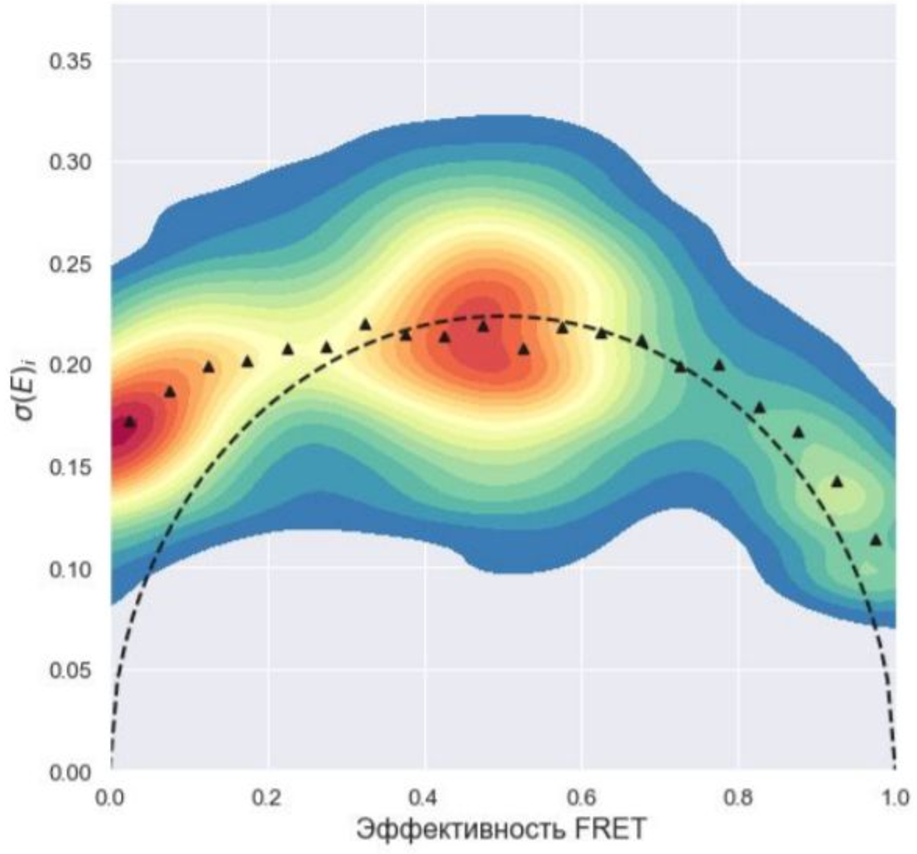
\includegraphics[width=\textwidth]{images/p1/part1_5_fret/part1_5_fret_f6.pdf}
%      \caption{Двумерная гистограмма распределения стандартного отклонения величины эффективности spFRET. Пунктиром показана линия ожидаемого стандартного отклонения для сигнала, распределенного биномиально (Формула 10).}
%      \label{fig:p1_5_fret:f6}
%  \end{figure}
 
    % На приведенной двумерной гистограмме (Рис. 6) видно, что для низких и высоких величин эффективности FRET стандартные отклонения превышают теоретическую оценку. Этот эффект может свидетельствовать о наличии быстрых перестроек в этих субпопуляциях частиц, но также может быть связан с тем, что метод оценки вариабельности вспышек не учитывает уровень фона и другие корректировочные коэффициенты (см. Формулу 3).%not edited













\subsection{Методы геномного анализа в исследовании структуры хроматина}
% сделать на основе https://docs.google.com/document/d/1GcTfefw2HnJGGnGmaJP5w2JN1Jy8X2EyCjyOlxEbagU/edit?usp=sharing

    Для определения наличия физического контакта между последовательностями ДНК в трехмерной структуре генома были разработаны методы семейства -С: 3С, 4С, 5С, Hi-C \cite{fraser_overview_2015}. Эти методы основаны на химическом ``сшивании'' контактирующих в хроматине участков, фрагментации ДНК с образованием ``сшитых'' пар, лигирования фрагментов в этих парах с образованием гибридных молекул ДНК, детекции гибридных молекул (обнаружение молекулы, состоящей из последовательности А и последовательности В, говорит о физическом контакте локусов этих последовательностей в ДНК).
    Существует понятие ``разрешения'' метода Hi-C (см. Таблицу \ref{tab:p1:hic}). Его можно определить как минимальное расстояние (в парах оснований) между участками, на котором они отображаются на тепловую карту в разные ее точки (пиксели). Величина разрешения зависит от величины фрагментов, на которые рестриктазы разрезают ДНК (то есть от особенностей используемых рестриктаз, размеров и встречаемости в геноме их сайтов рестрикции), и от размера бина, выбираемого на стадии обработки данных Hi-C, но не полностью произвольного: для получения тепловой карты, адекватно представляющей трехмерную структуру изучаемого генома, необходимо выбирать размеры бинов из определенного диапазона, зависящего от размеров хромосом, глубины секвенирования и качества NGS-библиотеки \cite{pal_hi-c_2019}. От разрешения метода Hi-C зависит то, какие структуры в хроматине он может выявить. Оригинальный протокол метода, описанный в статье 2009 года \cite{lieberman-aiden_comprehensive_2009}, позволял достичь разрешения 4kb и выявлял, соответственно, в трехмерной структуре генома компартменты A и B (соответствующие активному и неактивному хроматину). В протоколах Hi-C, разработанных позже, достигалось, благодаря использованию других рестриктаз, большее разрешение - до одной килобазы. Это позволяло обнаружить так называемые топологически ассоциированные домены (ТАДы) \cite{dixon_topological_2012} и взаимодействия конкретных последовательностей друг с другом - то есть, физические контакты регуляторных элементов с регулируемыми ими генами, реализованные, как полагают современные исследователи, запетливанием ДНК. Однако этих разрешающих способностей все равно не достаточно, чтобы изучить супрануклеосомный уровень, на котором ранее предполагалось существование 30-нанометровой фибриллы \cite{pal_hi-c_2019}.
    
    Пролить свет на этот уровень смог метод Micro-C — модификация метода Hi-C, предполагающая использование на этапе фрагментации ДНК микрококковой нуклеазы, которая уничтожает линкерные участки, оставляя одни  нуклеосомы (этот метод можно рассматривать как синтез метода позиционирования нуклеосом с помощью микрококковой нуклеазы - MNase-seq \cite{cui_genome-wide_2012} - и Hi-C \cite{hsieh_mapping_2015}. Это позволяет оценивать частоту взаимодействия отдельных нуклеосом друг с другом, то есть разрешение метода достигает неизученного супрануклеосомного уровня (между 200bp и 4kb), устраняя так называемый ``пробел в разрешении'' (resolution gap). Интересно, что метод Micro-C тоже не обнаружил 30-нанометровую фибриллу, еще раз доказав необходимость дальнейших исследований структуры хроматина супрануклеосомного уровня. В работе, в которой впервые был предложен метод Micro-C, изучался геном дрожжей - \textit{S. cerevisiae}. 
    
    Параллельно Micro-C был разработан другой метод Hi-C высокого разрешения - in situ DNase Hi-C. С его помощью можно получить данные с разрешением около 1kb \cite{ramani_mapping_2016}. Однако этот метод, основанный на использовании фермента DNase I, неспецифически фрагментирующего ДНК на тетрануклеотиды, не является конкурентным для Micro-C в области изучения супрануклеосомной структуры хроматина, так как не уничтожает линкерную ДНК и, соответственно, не позволяет в отличие от Micro-C простым способом получить данные о частоте взаимодействия нуклеосом друг с другом. 
    Сам протокол Micro-C модифицировался после его изобретения. Примером могут служить работы \cite{hsieh_micro-c_2016} и \cite{ohno_sub-nucleosomal_2019}, в которых были впервые представлены модификации Micro-C:  Micro-C XL и Hi-Co, соответственно. Micro-C XL - метод, позволяющий получить качественные данные в мононуклеосомном разрешении, это достигается путем снижения шума за счет изоляции нерастворимого хроматина и использования помимо формальдегида длинных сшивающих агентов (кросслинкеров) - например, DSG и EGS. Метод Hi-Co специфичен тем, что с его помощью можно определить ориентацию нуклеосом (``O''  в названии - от Orientation). Это достигается с помощью особой биоинформатической обработки и использования не просто секвенирования спаренных концов, а секвенирования спаренных концов с тэгами (PET - paired-end tags \cite{fullwood_next-generation_2009}).
    
    \begin{table}[p]
\caption{Увеличение разрешения Hi-C подобных методов, благодаря использованию менее специфичных рестриктаз.}
	\label{tab:p1:hic}	
	\begin{tabularx}{\textwidth} { 
  | >{\raggedright\arraybackslash}X 
  | >{\centering\arraybackslash}X 
  | >{\raggedleft\arraybackslash}X 
  | >{\raggedleft\arraybackslash}X |}
  \hline
Протокол Hi-C & Рестриктазы & Сайты рестрикции & Размер сайта рестрикции\\
	\hline

Классический (Lieberman-Aiden et al., 2009) & HindIII, NcoI & AAGCTT, CCATGG & 6 пн \\
\hline
Sexton et al., 2012, Rao et al., 2014 & Dpn-II & GATC & 4 пн \\
\hline
COLA (Darrow et al., 2016) & CviJI & RCGY, R=A/G, Y=C/G & 3 пн \\
\hline
Micro-C (Hsieh et al., 2016) & MNase & Отсутствует. Эндо/экзо нуклеаза, почти полностью уничтожает линкерные участки ДНК &  - \\
\hline
in situ DNAse Hi-C (Ramani et al., 2016) & DNAse I & Отсутствует. Режет ДНК на тетранукеотиды & -  \\
\hline
\end{tabularx}
	 
\end{table}
    
    Следует отметить, что все методы -C являются статистическими и вероятностными, приблизительно оценивающими частоту взаимодействия большого количества фрагментов ДНК. Для получения биологически значимой информации с помощью метода Hi-C вообще и, в частности Micro-C, необходим тщательный биоинформатический анализ матриц взаимодействия: фильтрация  и нормализация данных, учет того — использовалась в методе клеточная популяция или единичная клетка (Single-Cell Hi-C/Micro-C \cite{nagano_single-cell_2013}). Для изучения супрануклеосомной структуры хроматина с помощью Micro-C необходимо дополнительно прибегнуть к его молекулярному моделированию с учетом последних достижений в вычислительной биофизики.

\begin{figure} [h!]
    \centering
    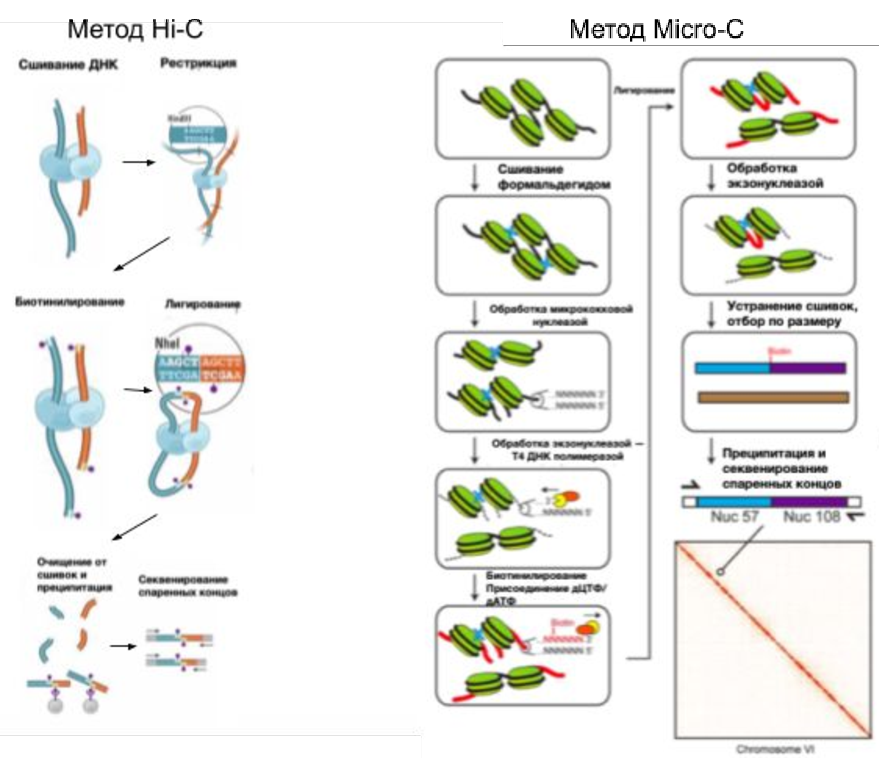
\includegraphics [width=\textwidth]{images/p1/part1_5_genome/p1_5_genome_f5.pdf}
    \caption[Методы ``захвата конформации хроматина''.]{Методы ``захвата конформации хроматина'' (chromatin conformation capture), сравнение Hi-C и Micro-C. Адаптировано из \cite{lieberman-aiden_comprehensive_2009} и \cite{hsieh_mapping_2015}.}
    \label{fig:p1_5_genome:f5}
\end{figure}


    Появление методов секвенирования нового поколения дало огромное преимущество большинству методов эпигеномики, позволяющим получать данные о местах расположения нуклеосом, в том числе с гистоновыми вариантами и с определенными пост-трансляционными метками гистонов. 

    Метод MNase-seq позволяет получить данные о расположении единичных нуклеосом. В методе используется микрококковая нуклеаза, которая обладает экзо- и эндонуклеазными активностями. После работы нуклеазы, нуклеосомальная ДНК освобождается от гистонов и секвенируется. Далее прочтения картируются на референсный геном.       На данный момент в публичном доступе накоплено большое количество экспериментальных наборов данных для клеток разных организмов и из разных тканей человека (110 наборов данных по данным сайта \url{https://generegulation.org/nucleosome-positioning-database/}).
    К основным проблемам использования методов Mnase-seq относится огромное количество получаемых с одного эксперимента прочтений - порядка 200-400 млн для клеточных линий человека. Для достижения оптимального разрешения позиционирования нуклеосом в человеческих клетках для сравнения здоровых и больных требуется порядка 1-4 млрд прочтений \cite{teif_nucleosome_2016}. Обычно эксперименты MNase-seq выполняют на нескольких тысячах клеток, такой усредненный нуклеосомальный профиль характеризует ансамбль клеток, а не частные состояния клеток. Специализированная база данных NucMap включает 798 экспериментальных наборов данных MNase-seq из 477 образцов для 15 видов живых организмов \cite{zhao_nucmap:_2019}. Для дрожжей существует метод СС-seq, позволяющий определять позиционирование нуклеосом с большей точностью, чем MNase-seq \cite{brogaard_map_2012}. Суть метода в ведении специальной мутации в гистоны, в результате которой вблизи центра нуклеосомы появляется остаток цистеина. Боковая цепь цистеина используется для реакции со специальными химическими агентами, которые разрезают ДНК в центре нуклеосомы. Далее методами секвенирования определяется положение разреза и, следовательно, центра нуклеосомы.
    Методы ChIP-seq осуществляют анализ ДНК-белковых взаимодействий. 
    В открытом доступе находится большое количество наборов данных ChIP-seq гистоновых модификаций, включая метки энхансеров и промотеров, например, ChIPBase v.2.0 2466 датасетов, IHEC Data Portal - несколько тысяч образцов из разных человеческих органов, ChIP-Atlas - данные из 96000 экспериментов. Также ChIP-Atlas позволяет ответить на следующие вопросы: какие белки были связаны с определенной последовательностью ДНК, какие гены регулируются данным белком, какие белки колокализированы с данным, а также позволяет предсказывать белки, связанные с данными геномными локусами и генами (in silico ChIP).
    Важная модификация метода ChIP-seq - метод Mnase ChIP-seq заключается в отщеплении свободных п.н. (линкерной ДНК) микрококковой нуклеазой до этапа иммунопреципитации. В результате образуются фрагменты 20-70 п.н., позволяющие строить нуклеосомальные профили и выявлять сайты связывания транскрипционных факторов высокого разрешения.  Было отмечено, что MNase-ChIP-seq также позволяет увеличить воспроизводимость результатов по сравнению с ультразвуковой фрагментацией в методе ChIP-seq \cite{wedel_genome-wide_2017}. 
    В работе \cite{rhee_subnucleosomal_2014} с помощью методов ChIP-exo и MNase-seq было показано наличие субнуклеосомальных структур (гексасомы, нуклеосомы с единично представленными гистонами типов H2A, H2B, H3, H4) \textit{in vivo} и сделаны предположения о влияния последовательности ДНК на образование таких структур. 

    В работе \cite{quintales_comparative_2015} проведено сравнение обработки сырых данных экспериментов: MNase-seq, ChIP-seq и метода химического расщепления ДНК в месте диадной оси, используя разные стратегии секвенирования (одноконцевое и парноконцевое), с помощью разработанной программы NUCwave. Было показано, что обработка данных парноконцевого секвенирования MNase-seq наиболее точно определяет известные позиции нуклеосом и превосходит другие сырые данные для построения карт расположения нуклеосом.

\begin{figure} [h!]
    \centering
    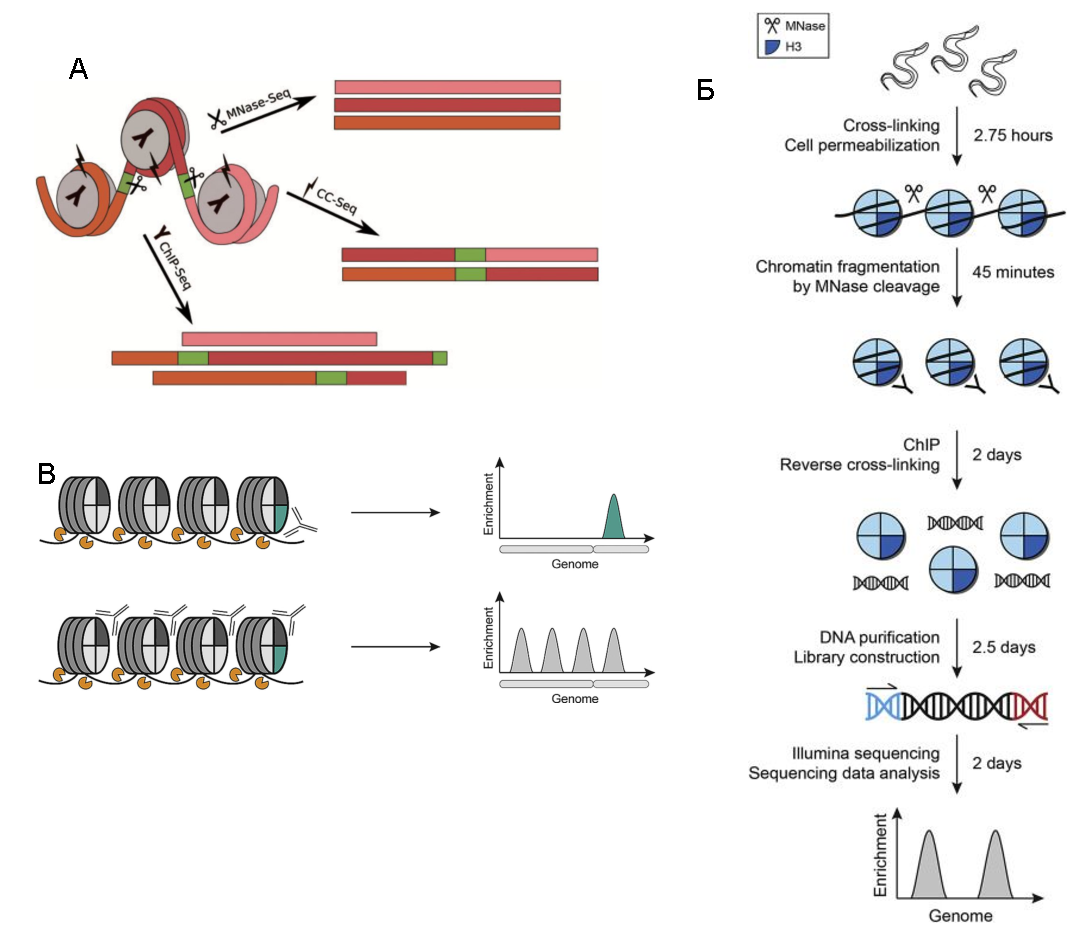
\includegraphics [width=\textwidth]{images/p1/part1_5_genome/p1_5_genome_f6.pdf}
    \caption[Методы эпигеномики нуклеосомного разрешения]{Методы эпигеномики нуклеосомного разрешения: А) MNase-seq, ChIP-seq, CC-seq. Б-В) MNase-ChIP-seq. Адаптировано из \cite{quintales_comparative_2015} и \cite{wedel_genome-wide_2017}.}
    \label{fig:p1_5_genome:f6}
\end{figure}



















%\subsection{Кристаллография}
%\subsection{Электронная микроскопия}
%\subsection{ЯМР}
%\subsection{Малоугловое рассеяние}
%\subsection{Методы дейтеро-водородного обмена}
%\subsection{Лазеры на свободных электронах}




\section{Выводы главы \ref{chapt1_mod_methods}}
Исследование структуры многих биомакромолекулярных комплексов испытывает затруднения как при применении стандартных методов структурной биологии, так и при попытках атомистического моделирования на основе расчета атом-атомных взаимодействий. Методы интегративного моделирования, в ходе расчетов учитывающие как физические взаимодействия между атомами, так и экспериментальные данные различной природы, являются перспективным подходом для построения структурно-динамических моделей биомакромолекулярных комплексов. В главе предложены подходы по моделированию ДНК-белковых комплексов на основе моделей анизотропной гибкости ДНК с учетом разнородных экспериментальных данных.
%\subsection{Положения выносимые на защиту}
%положения выносимые на защиту
% \begin{enumerate}
%   \item Охарактеризовано направление интегративного моделирования, как набор подходов атомистического и огрубленного моделирования, позволяющих создавать структурно-динамические модели биомакромолекул и их комплексов на основе наборов разнородных экспериментальных данных.
%   \item Предложены комплексные подходы по моделированию структуры и динамики ДНК-белковых комплексов с учетом разнородных экспериментальных данных, в том числе низкого информационного содержания.
% \end{enumerate}
 
